\documentclass[12pt]{article}
\usepackage{graphicx,rotating}

\oddsidemargin  -0.5 cm
\evensidemargin 0.0 cm
\textwidth      6.5in
\headheight     0.0in
\topmargin      -1 cm
\textheight=9in

\newcommand{\s}[1]{{\mbox{\scriptsize #1}}}

\title{Summer 2010 Beam-Halo Overlaps Alignment}
\author{Jim Pivarski}

\begin{document}
\maketitle

\section{Motivation}

The ``Beam-Halo Overlaps Alignment Method'' aligns CSC chambers
relative to their neighbors within rings using beam-halo tracks that
cross pairs of neighboring chambers.  The method has been applied to
the following datasets:
\begin{itemize}
\item Sep.~2008: ``first beam'' (9 minutes) with $\vec{B}=0$~T, only
  two rings with zero missing overlaps (ME$-$2/1, ME$-$3/1), not
  uploaded to the database;
\item Dec.~2009: ``first collisions'' (21 days) with $\vec{B}=3.8$~T,
  too few tracks for any alignment due to clean, low-intensity beams;
\item Mar.~2010: ``Tertiary Collimator Triplet (TCT) test'' (40
  minutes) with $\vec{B}=3.8$~T, new technique uses photogrammetry
  to fill in missing overlaps, aligned all chambers and uploaded
  to the database;
\item Jun.--Sep~2010: beam-halo during collisions (83 days) with
  $\vec{B}=3.8$~T, repeated with \mbox{$\sim 10\times$} the statistics
  and new $\phi_y$ alignment derived from collisions to reduce a
  systematic error.  Proposed for upload to the database (with
  upcoming disk alignment).
\end{itemize}
This short note describes the last alignment, using data collected by
the beam-halo trigger during the most intense LHC beams before the
trigger was retired on Sep.~1.

This alignment is only one step in a sequence of endcap alignment
steps:
\begin{enumerate}
\item photogrammetry pre-alignment (local $x$, $y$, $z$, $\phi_x$, $\phi_z$);
\item SLM lines measurement of disk displacement and bending due to
  the magnetic field (local $z$, $\phi_x$, replacing photogrammetry);
\item ``missing angle measurement'' from collisions (local $\phi_y$);
\item beam-halo alignment of chambers relative to rings, combined with
  PG to fill in data in missing chambers ($r\phi \approx x$ and $\phi_z$, replacing photogrammetry);
\item disk alignment using collisions (global $x$, $y$, $\phi_z$ of
  whole disks, keeping internal chamber structure intact, for YE1 and
  YE2);
\item disk alignment using straight-through collisions (global $x$,
  $y$, $\phi_z$ of whole disks for YE3 relative to YE2).
\end{enumerate}

\section{Reminder of the method}

CSC chambers in each station overlap each other slightly along their
edges, in part to provide short tracks for alignment.  Tracks passing
through the overlap region do not encounter any thick material, so
their trajectories can be accurately propagated between the chambers.
Track-segments constructed from hits in each chamber individually are
linearly extrapolated to a plane equidistant between them, and the
$r\phi$ difference between their points of intersection is called the
overlap residual.  A bias in the distribution of overlap residuals
indicates a relative misalignment of the two chambers.
Figure~\ref{fig:overlaps} summarizes these definitions.

\begin{figure}
\begin{center}
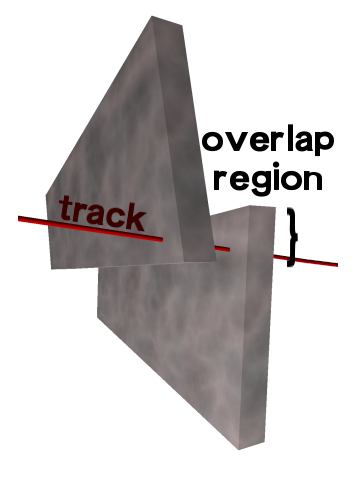
\includegraphics[height=4.5 cm]{overlaps.png}\hspace{0.5 cm}
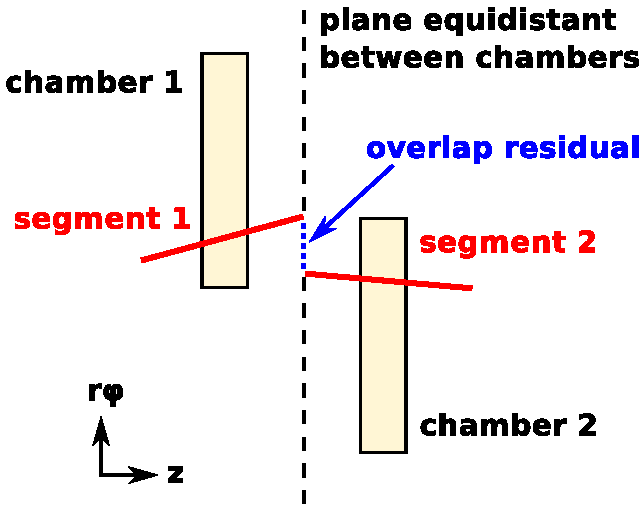
\includegraphics[height=4.5 cm]{overlaps_diagram.pdf}\hspace{0.5 cm}
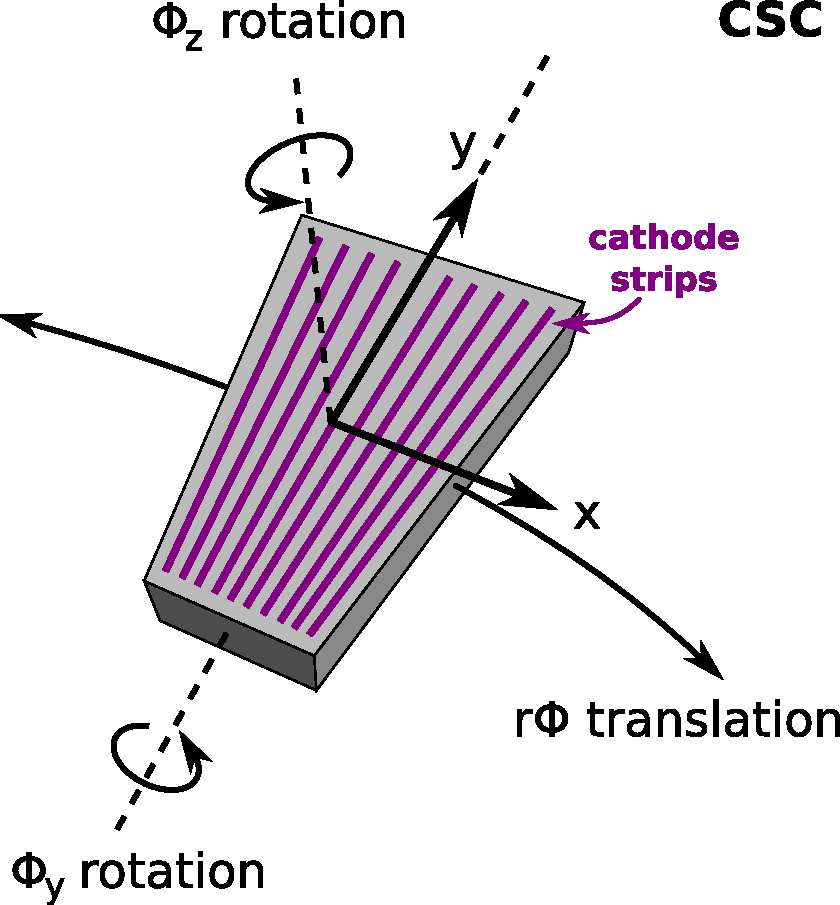
\includegraphics[height=4.5 cm]{csc_coordinates.pdf}
\end{center}
\caption{Left: illustration of a track passing through the overlap
  region.  Middle: diagram indicating how the overlap residual is
  defined.  Right: coordinates of a chamber position that are relevant
  for this alignment. \label{fig:overlaps}}
\end{figure}

To compute relative corrections to the positions of all chambers in a
ring from these pairwise constraints, we minimize the following:
\begin{equation}
\chi^2 = \sum_{m_{ij}}^\s{constraints} \frac{(m_{ij} - A_i +
  A_j)^2}{{\sigma_{ij}}^2} + \lambda \left(\frac{1}{N_\s{chambers}} \sum_i^\s{chambers}A_i\right)^2
\label{eqn:minimizeme}
\end{equation}
where $m_{ij}$ is a constraint between chambers $i$ and $j$ and
$\sigma_{ij}$ is its uncertainty (the constraint is statistically
satisfied if $|m_{ij}/\sigma_{ij}| \sim 1$), $A_i$ and $A_j$ are
chamber position corrections, and the last term is a Lagrange
multiplier to make the system solvable by enforcing an arbitrary
coordinate system ($\lambda$ is an arbitrary constant: the only
alignment results that are physically meaningful do not depend on $\lambda$).
Beam-halo tracks (BH) provide one of the two sets of constraints: the
mean of each overlaps residuals distribution is required to be zero.
Since tracks in CSC overlap regions only relate chambers relative to
their immediate neighbors, each of these constraints relates chambers
$i$ and $j=i+1$ (or $j=1$ if $i=N_\s{chambers}$).

The above formalism would be sufficient to align all chambers in a
ring if no overlaps were missing.  However, several of the 400
chamber-overlaps in the muon endcap are not read out due to
electronics issues (see next section).  Photogrammetry (PG)
measurements from 2007 supplement the beam-halo data in order to fill
in the gaps.  PG constraints relate each chamber $i$ with an external
reference, treated as a new alignable $A_\s{PGFrame}$.  PG data are
applied in two ways: (1)~all available PG data are included in the
fit, weighted appropriately with BH according to their uncertainties,
and (2)~only PG measurements necessary to fill gaps in BH are applied.

Figure~\ref{fig:beamhalo-PG} illustrates this procedure as a graph:
only fully connected graphs are solvable.  Sometimes we wish to study
the alignment of a disconnected graph (e.g.\ ME1/1 and alignments
without PG constraints); in those cases, we add a Lagrange multiplier
(with separate $\lambda_i$) for each missing overlap.  Disconnected
groups are said to ``float freely'' with respect to one another
($\lambda_i$ may be tuned arbitrarily: it does not represent a real
alignment result).

\begin{figure}
\begin{center}
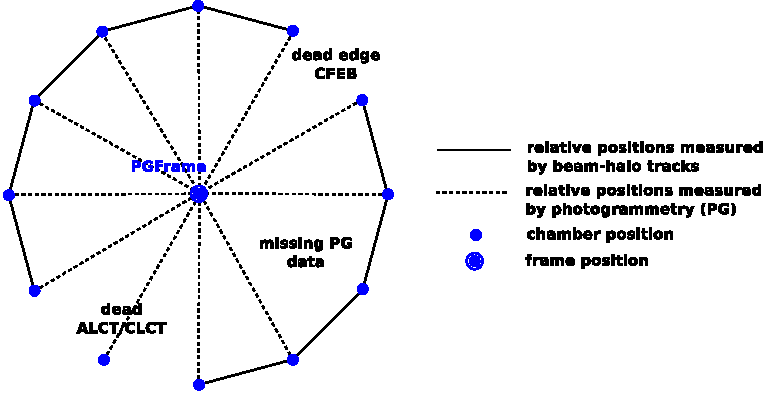
\includegraphics[width=0.9\linewidth]{beamhalo-PG.pdf}
\end{center}
\caption{Schematic diagram showing how beam-halo (BH) and
  photogrammetry (PG) data are combined.  Each point represents an
  alignable $A_i$ (most of which are chambers, one is an abstract
  point ``PGFrame'') and each edge represents a measurement constraint
  $m_{ij}$ between alignables $A_i$ and $A_j$.  Alignment of all
  alignables in a single coordinate system is possible if the graph is
  fully connected.  Otherwise, coordinate systems for each connected
  subgraph ``float freely'' with respect to one another. \label{fig:beamhalo-PG}}
\end{figure}

The objective function in Eqn.~\ref{eqn:minimizeme} is minimized by
setting its derivatives to zero, which forms an
$N_\s{alignables}\times N_\s{alignables}$ matrix where
$N_\s{alignables} = 18\mbox{ or }36$, and numerically solving the
resulting matrix equation.  The chamber corrections $A_i$ in the
solution are highly correlated, but the correlated statistical
uncertainties can be decomposed into a set of statistically
independent modes.  That is, the vector $\vec{A}$ can be written in a
new basis as $\vec{B}$, in which each $B_i$ is a linear combination of
all $A_i$ and graphically looks like a coherent, global distortion of
the entire ring.  The change of basis was designed such that each
$B_i$ has a statistically independent uncertainty.  The $B_i$ with the
largest uncertainties are called the weakest modes.

\section{Details of the dataset and method}

\subsection{Summer 2010 dataset}

Unlike previous beam-halo alignments, the summer 2010 data were
collected over a long time period, while the beams were colliding.  A
special trigger was designed to collect beam-halo data during
collisions, though the beam-halo AlCaReco stream accepted muons from
all muon triggers (``{\tt HLT\_CSCBeamHaloOverlapRing1 OR
  HLT\_CSCBeamHaloOverlapRing2 OR \\ HLT\_L1Mu* OR HLT\_L2Mu* OR
  HLT\_Mu* OR HLT\_L1MuOpen*}''), so it is possible that some of the
muons used in this analysis were from $pp$ collisions, rather than
beam-halo.  It is not necessary for the sample to be purely
beam-halo--- only the topology is important: nearly horizontal tracks
with relatively high momentum.

Figure~\ref{fig:occupancy_March2010} presents the occupancy
distribution of CSC overlaps with the March 2010 TCT test (pure
beam-halo in a 40-minute run) as a reference.  Note that each
``overlap'' corresponds to a pair of chambers, not a single chamber
(so a whole missing chamber results in two missing overlaps).  Every
missing overlap (zero or only several hits) was diagnosed in
March; each had a cause that could be traced to an electronics issue.
In the summer data, seven of the ME1/1 overlaps were fixed (5 with low
HV in a single layer, 2 with low CFEB efficiency on the edge of a
chamber), and one new problem was introduced in ME$-$1/2.  This change
in the pattern of missing chambers in ME1/1 significantly affected the
results (where gaps are not controlled by PG).

\begin{sidewaysfigure}[p]
\begin{center}
\begin{minipage}{0.45\linewidth}
\begin{center}
March 2010 (40-minute LHC TCT test)
\end{center}
\end{minipage}
\begin{minipage}{0.45\linewidth}
\begin{center}
Jun--Sep 2010 (beam-halo during collisions)
\end{center}
\end{minipage}

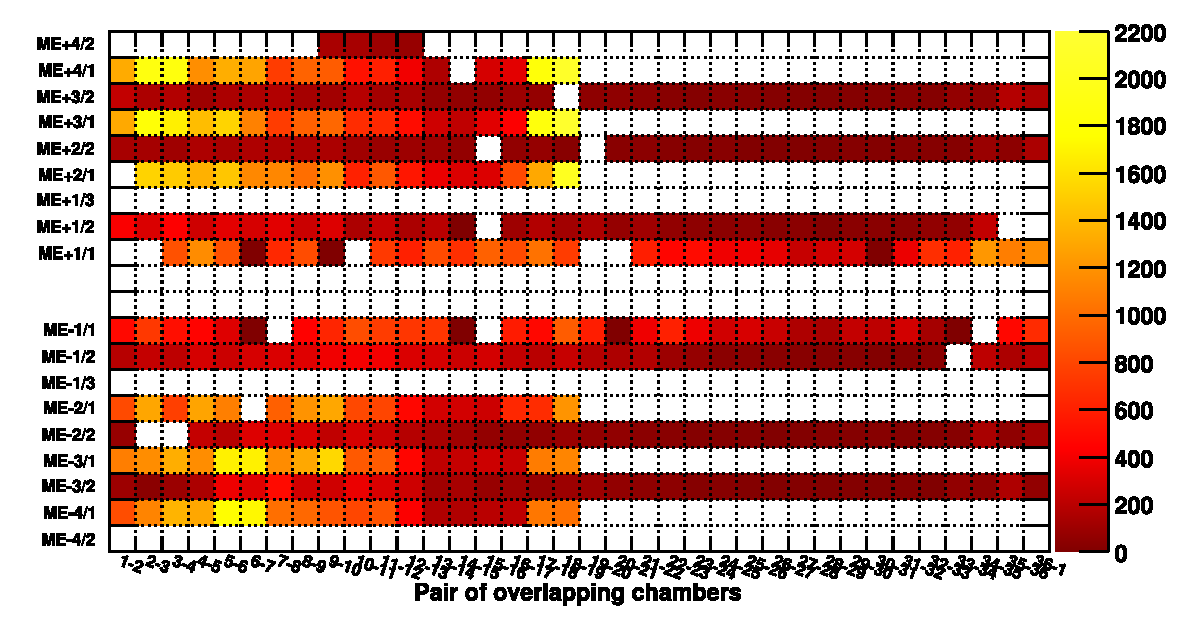
\includegraphics[width=0.45\linewidth]{occupancy_March2010.pdf}
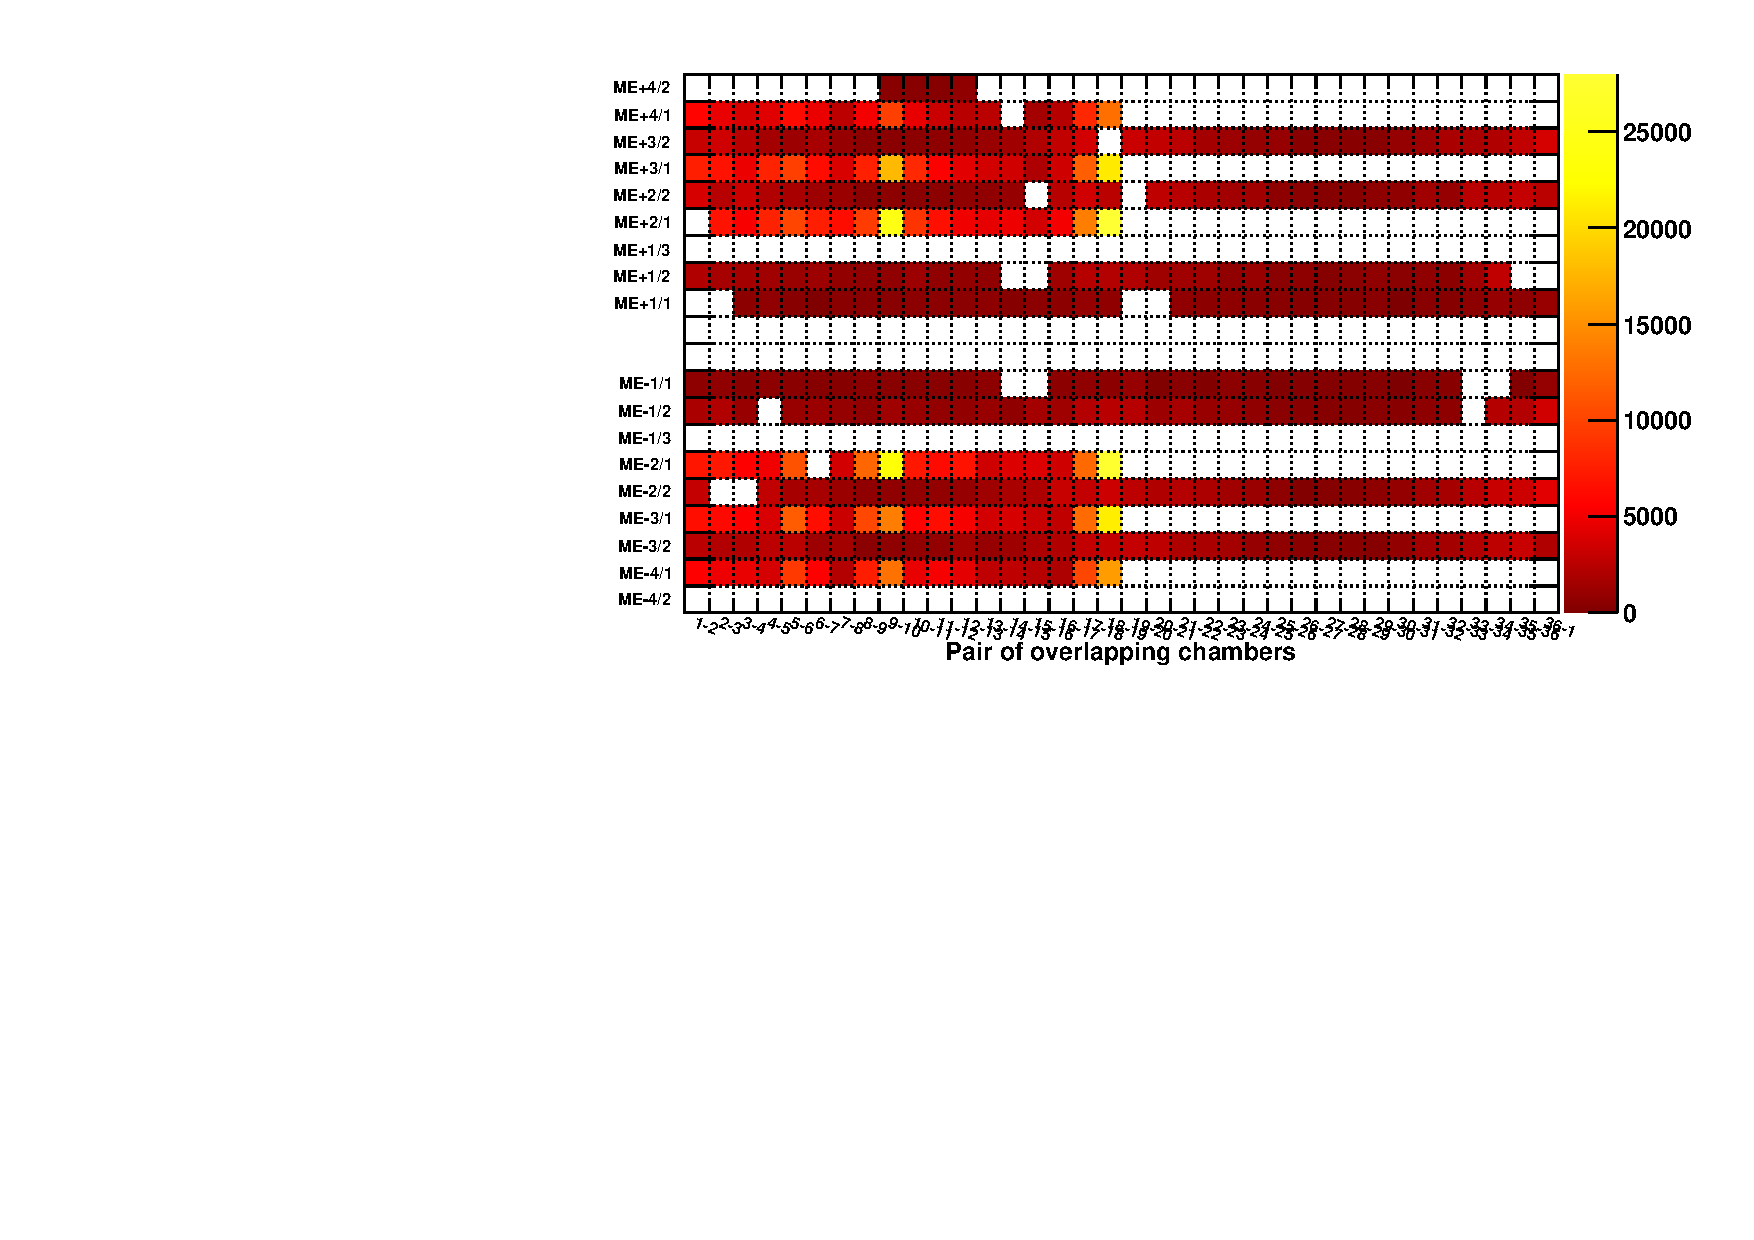
\includegraphics[width=0.45\linewidth]{occupancy_Oct2010.pdf}

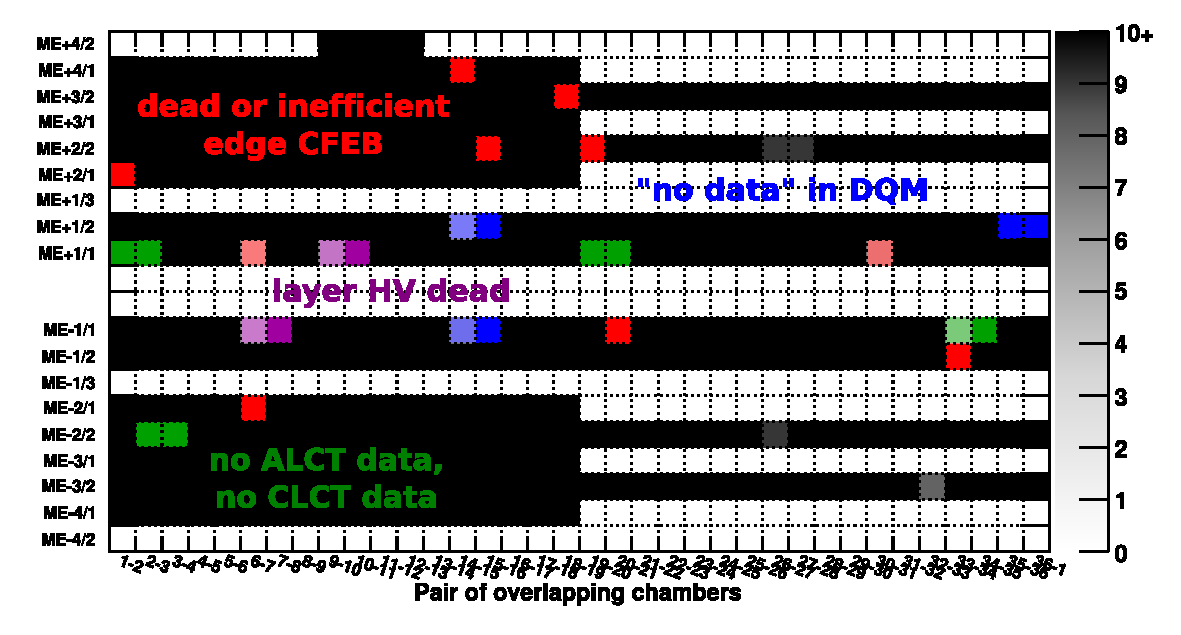
\includegraphics[width=0.45\linewidth]{occupancy_problems_March2010.pdf}
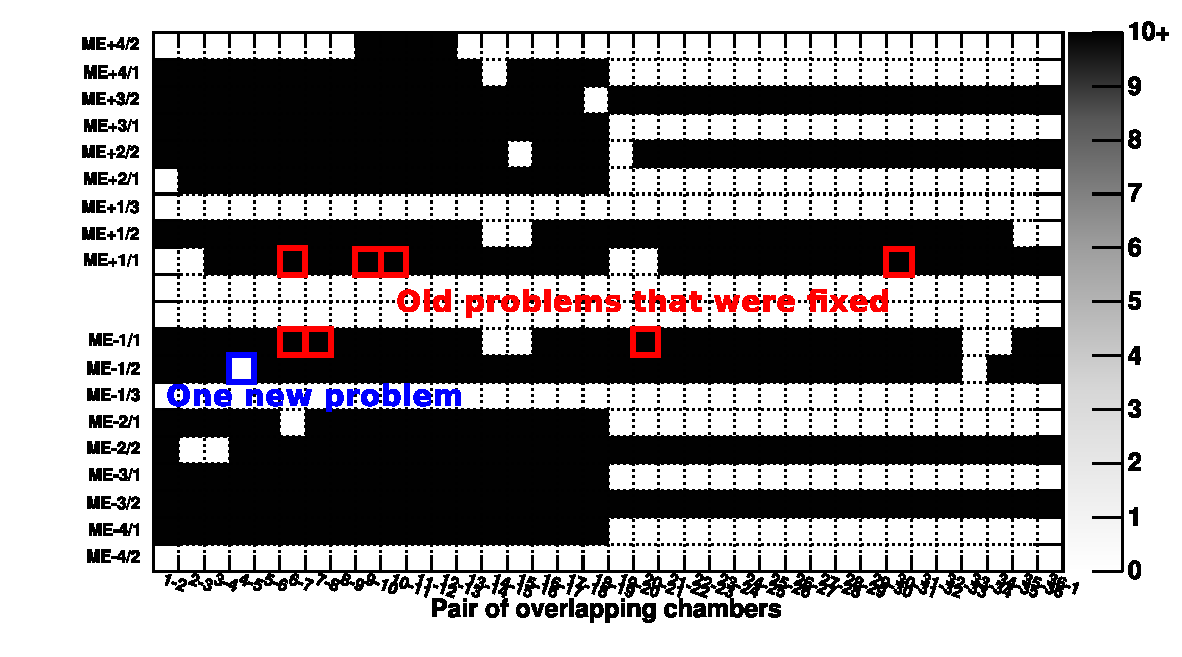
\includegraphics[width=0.45\linewidth]{occupancy_problems_Oct2010.pdf}
\end{center}
\caption{Occupancy maps of CSC chambers during the March special
  beam-halo run (left) and the most intense period of beam with the
  beam-halo-during-collisions trigger (right).  The top plots show
  number of hits in the color scale and the bottom plots show the same
  with a color scale saturated by 10 or more hits, to identify
  inactive CSCs.  Each inactive CSC was diagnosed in March (reasons
  for no read-out are given on the plot).  In the summer data, 7
  previously inactive ME1/1 chambers are now reading out data, and 1
  previously active ME$-$1/2 chamber is now
  inactive. \label{fig:occupancy_March2010}}
\end{sidewaysfigure}

\subsection{Selection criteria}

To select well-behaved muons (muons whose trajectory can be accurately
propagated from one chamber to its neighbor), we require the muons to
have momenta of several tens of GeV/$c$ or higher.  Horizontal muons
are parallel with the axial magnetic field of CMS, so all momentum
information comes from the radial component of the magnetic field.  To determine how well
true momentum can be estimated from the offline track-fit, an MC
sample of horizontal muons was simulated.
Figure~\ref{fig:trackfit_resolution}-a shows the distribution of
reconstructed momenta as a function of true momentum, and
Fig.~\ref{fig:trackfit_resolution}-b shows the efficiency of a
reco-level cuts as a function of true momentum.  With a 20~GeV/$c$
reco-level cut, the efficiency for 10~GeV/$c$ muons is less than 20\%,
dropping to zero efficiency for very low-momentum muons.
Figure~\ref{fig:trackfit_resolution}-c shows the reco-level momenta in
data with the $|\vec{p}| < 20$~GeV/$c$ cut used in the analysis.

\begin{figure}
\begin{center}
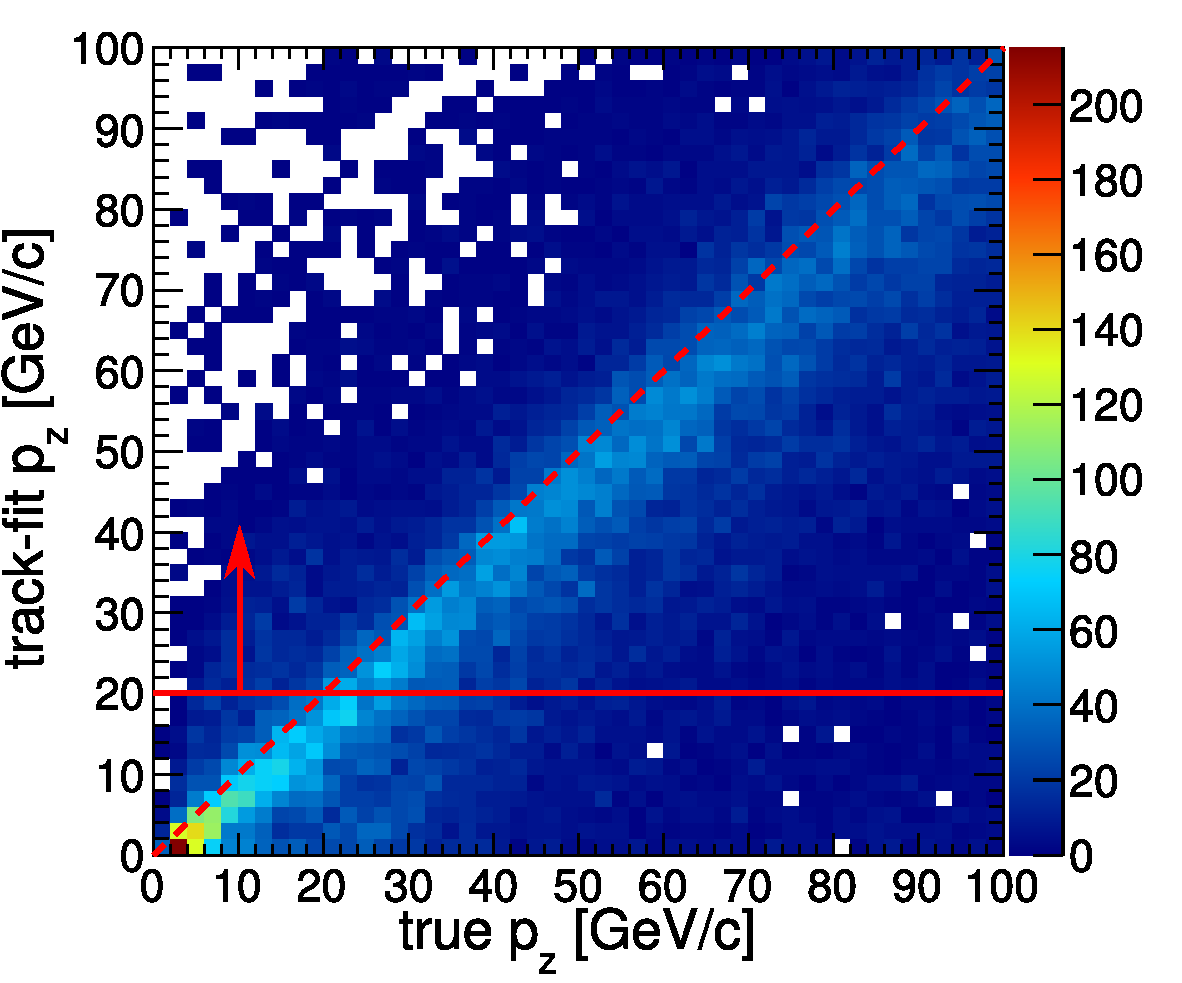
\includegraphics[height=6 cm]{trackfit_resolution.pdf}\hfill
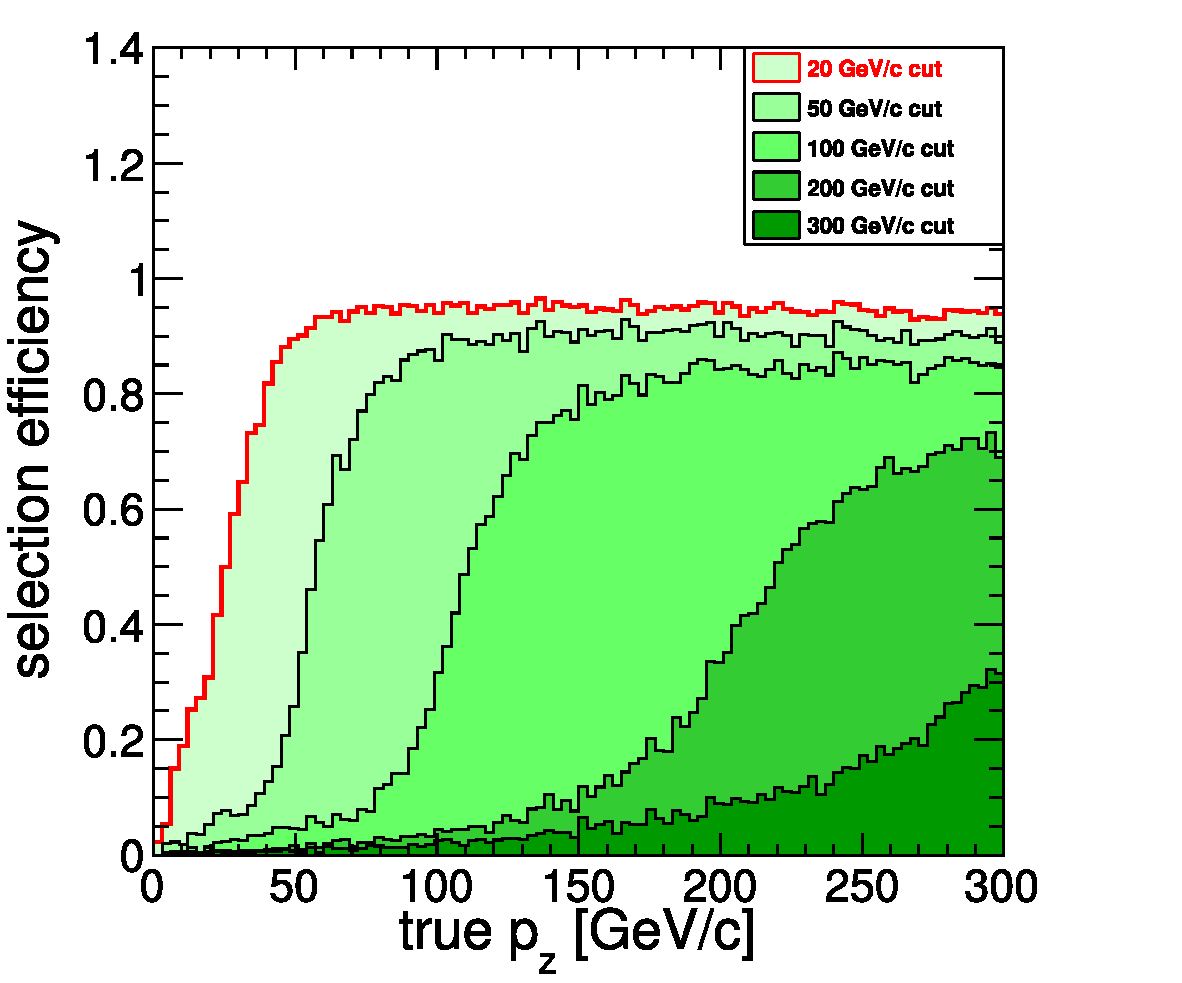
\includegraphics[height=6 cm]{trackfit_turnon.pdf}

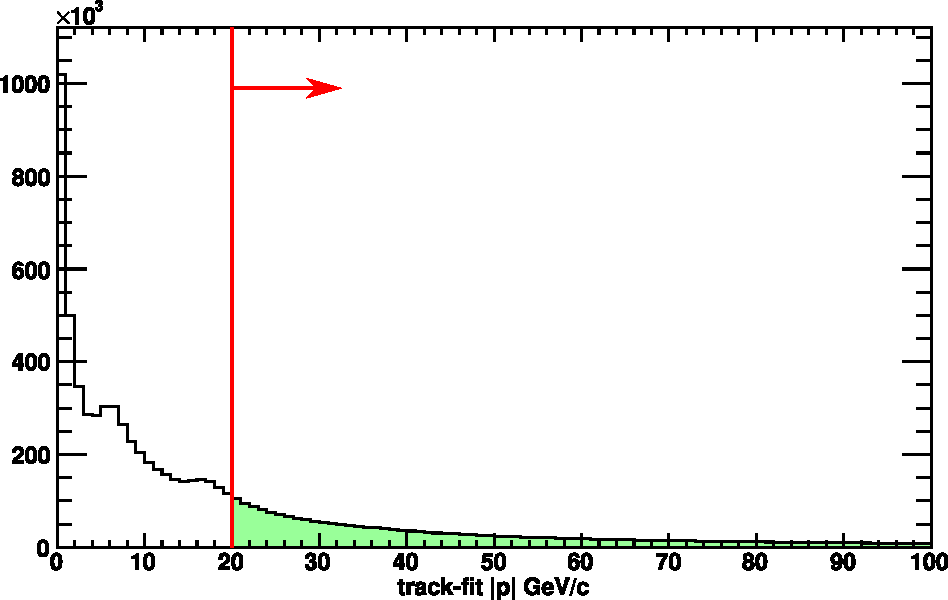
\includegraphics[height=5 cm]{momentum_Oct2010.pdf}
\end{center}
\caption{Top-left: reconstructed track momentum ($p_z$) versus true
  track momentum in MC.  Top-right: efficiency as a function of true
  track momentum with a $p_z > 20$~GeV/$c$ cut in MC.  Bottom:
  distribution of reconstructed track momentum ($|\vec{p}|$) in
  data. \label{fig:trackfit_resolution}}
\end{figure}

To select horizontal muons, we applied a cut on the entrance angle of
track-segments in the $r$-$z$ plane.  This angle may be described as
$dr/dz$ where $r$ is the radius of hits in the segment and $z$ is the
component parallel with the beamline.  Muons from the interaction
point have $|dr/dz| > 0.12$~rad, which corresponds to $|\eta| < 2.4$
($|dr/dz| \to \infty$ implies $\eta \to 0$).
Figure~\ref{fig:drdz_Dec2009} presents the $dr/dz$ distribution
observed in three datasets: Dec.~2009 (which had an open trigger and
was dominated by cosmic rays), Mar.~2010 (which had an open trigger
and was dominated by beam-halo), and summer~2010 (which had a tight
trigger and contains both beam-halo and collisions).  A $|dr/dz| <
0.2$~rad cut was used in the Mar.~2010 analysis, but this cut was
tightened to $|dr/dz| < 0.12$ for the analysis described in this note,
to exclude muons that point to the beamspot.

\begin{figure}
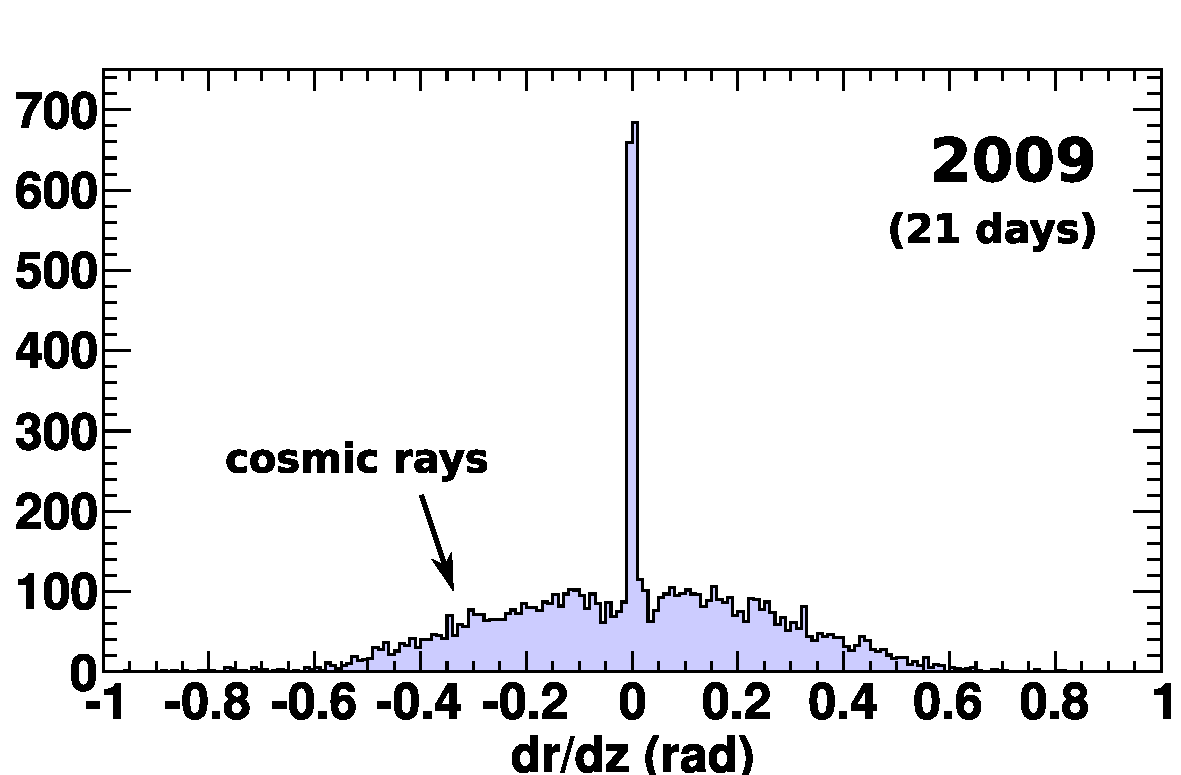
\includegraphics[height=3.5 cm]{drdz_Dec2009.pdf}
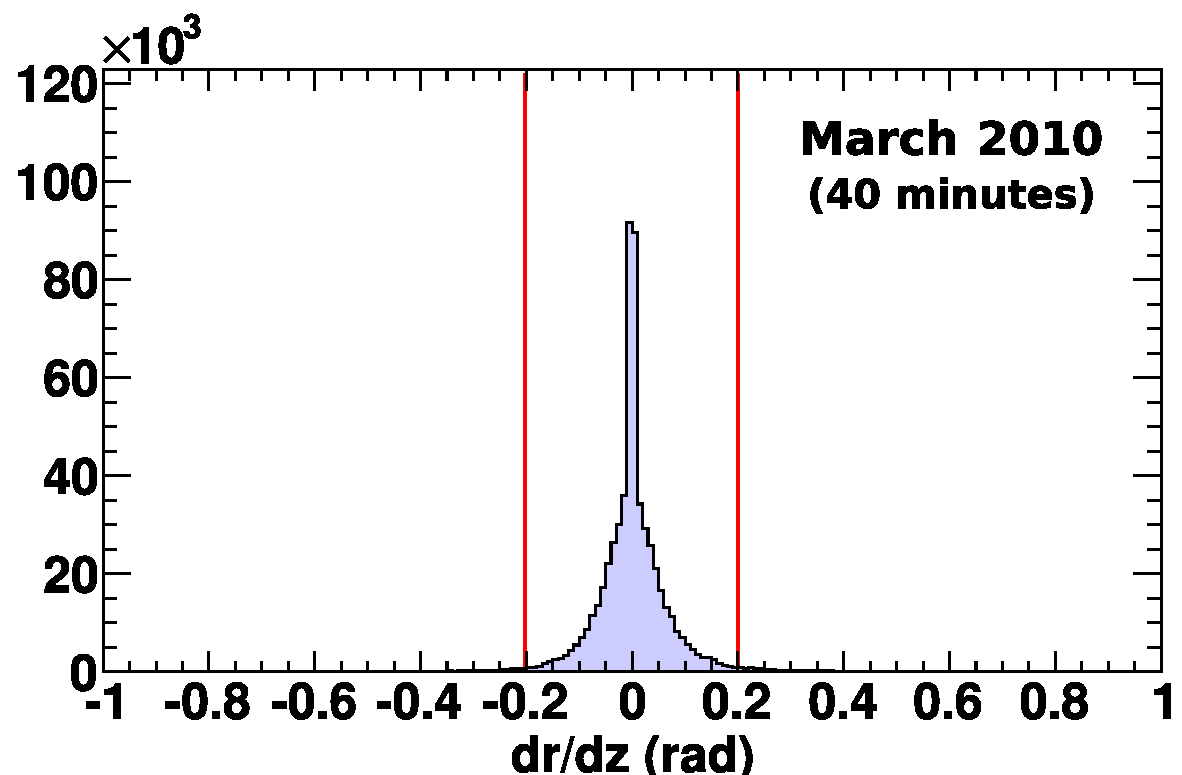
\includegraphics[height=3.5 cm]{drdz_March2010.pdf}
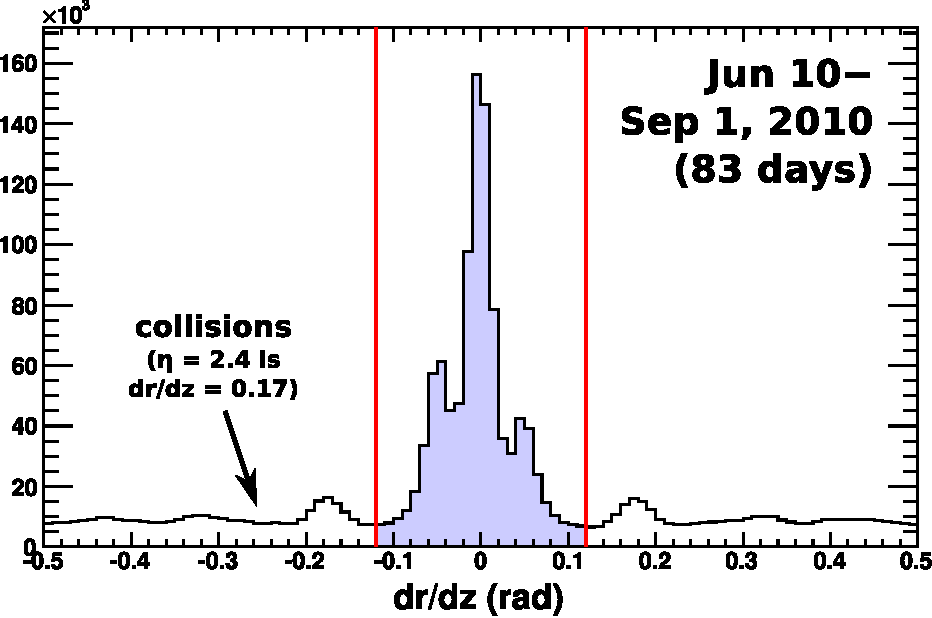
\includegraphics[height=3.5 cm]{drdz_Oct2010.pdf}

\caption{Track entrance angles $dr/dz$ where $r$ is the radial
  component and $z$ is parallel with the beamline, for 2009 data
  (left), March 2010 data (middle), and summer 2010 data (right, with
  a narrower window).  Each has different background components and
  different trigger conditions. \label{fig:drdz_Dec2009}}
\end{figure}

Tracks and hits used in this analysis also required the following:
\begin{itemize}
\item at least 5 hits per chamber (which has 6 layers);
\item fitted track-segment must stay within the fiducial region of
  each chamber: $|\phi| < 0.086$ for ME1/1, $|\phi| < 0.090$ for
  ME1/2, $|\phi| < 0.180$ for ME$x$/1, and $|\phi| < 0.090$ for
  ME$x$/2, where $\phi$ is the difference in azimuthal position
  between the track-segment position and the center of its chamber and
  $x \ge 2$;
\item ``offset residuals,'' the difference in propagated $r\phi$
  position at the common plane between the two chambers, must have a
  magnitude less than 15~mm;
\item ``slope residuals,'' the difference in $d(r\phi)/dz$ angle for
  the two track-segments in an overlap, must be less than 30~mrad.
\end{itemize}
Figure~\ref{fig:offsetResiduals_badphiy} presents the offset residuals
and slope residuals, with and without $\phi_y$ pre-alignment.  Since
most of the $\phi_y$ corrections were only a few mrad and the overlaps
measurement has a resolution of 8~mrad, the improvement is not
visible.

%% hits_Oct2010.pdf

\begin{figure}
\begin{center}
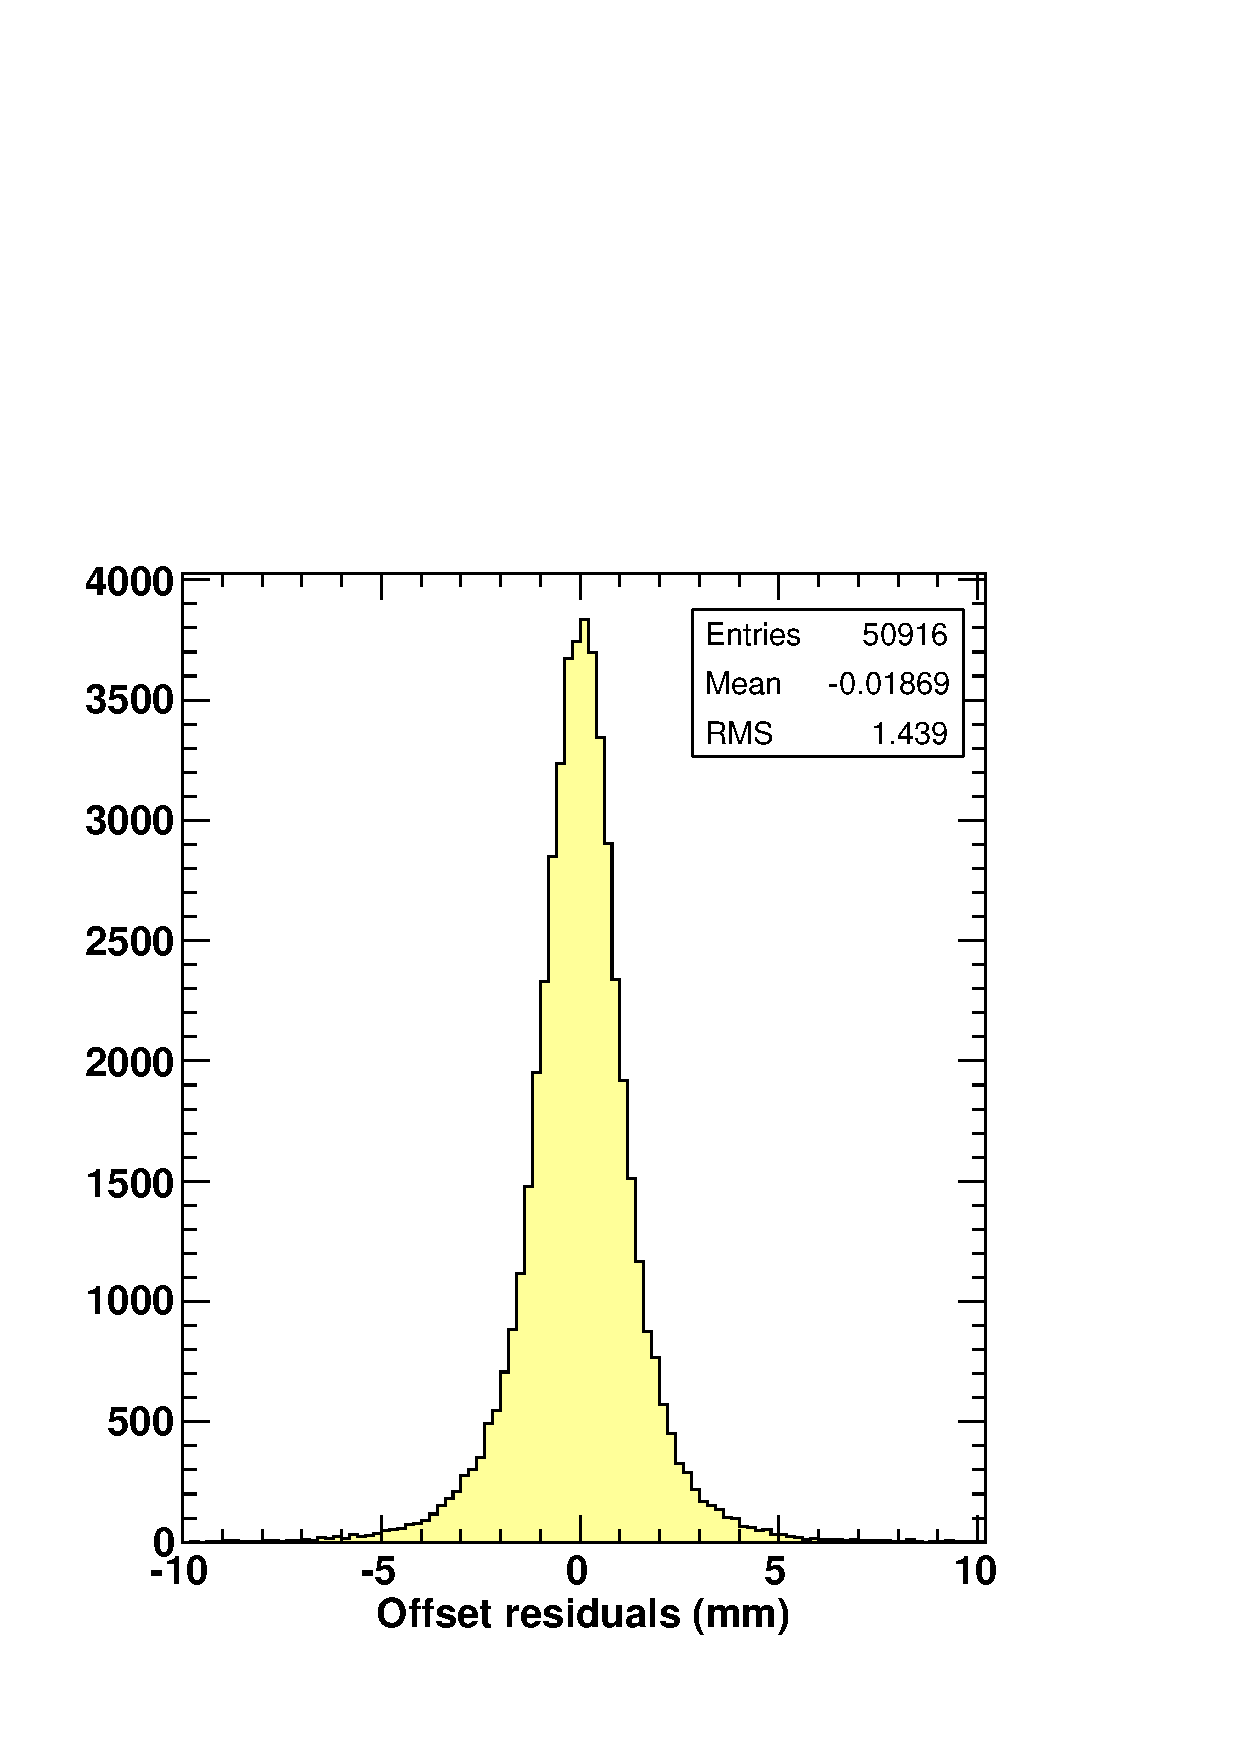
\includegraphics[width=0.35\linewidth]{offsetResiduals_badphiy.pdf}\hspace{1 cm}
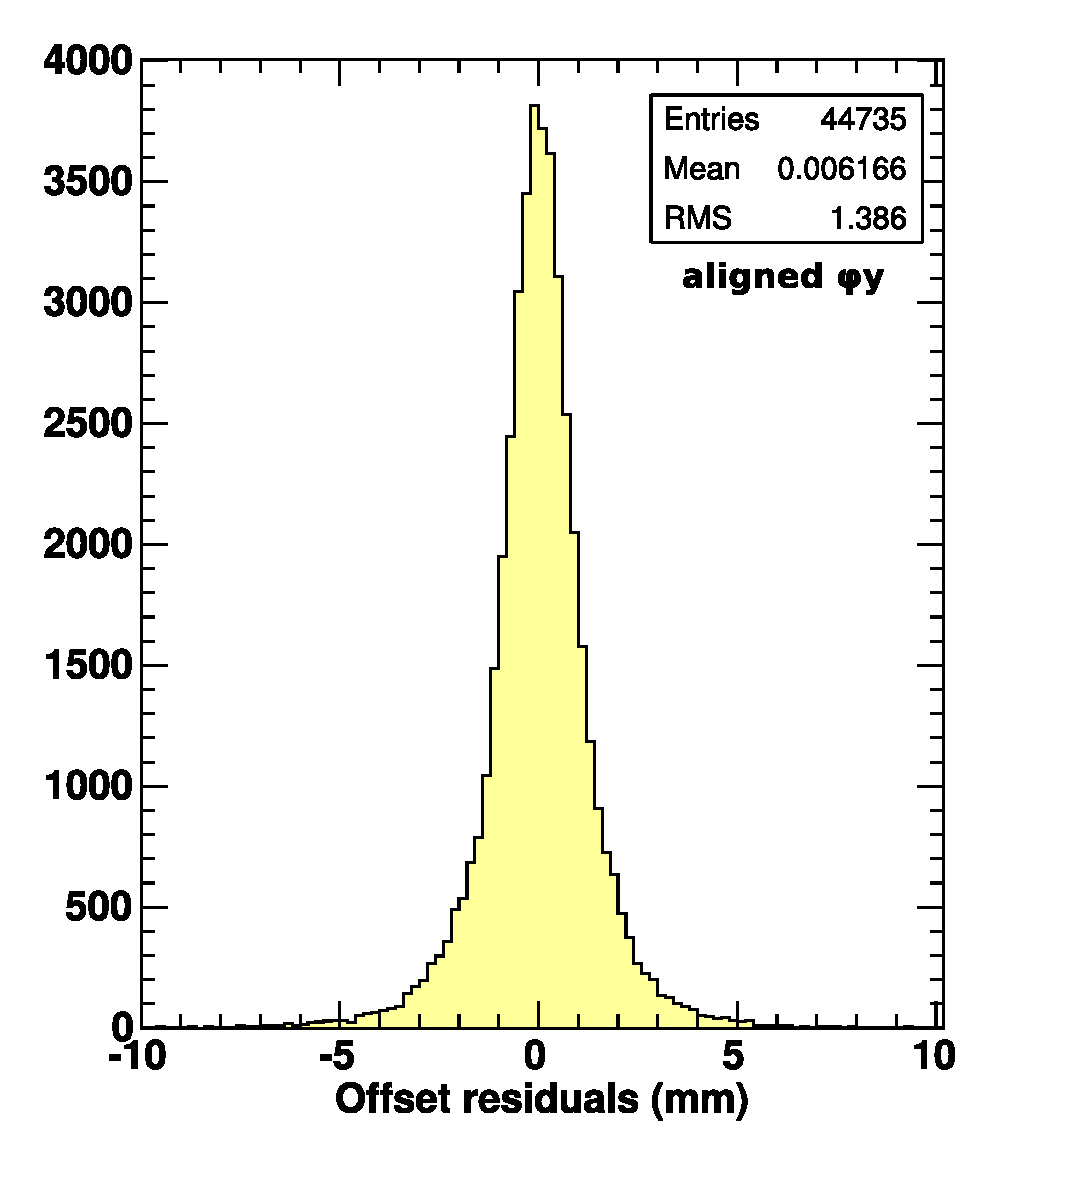
\includegraphics[width=0.35\linewidth]{offsetResiduals_goodphiy.pdf}

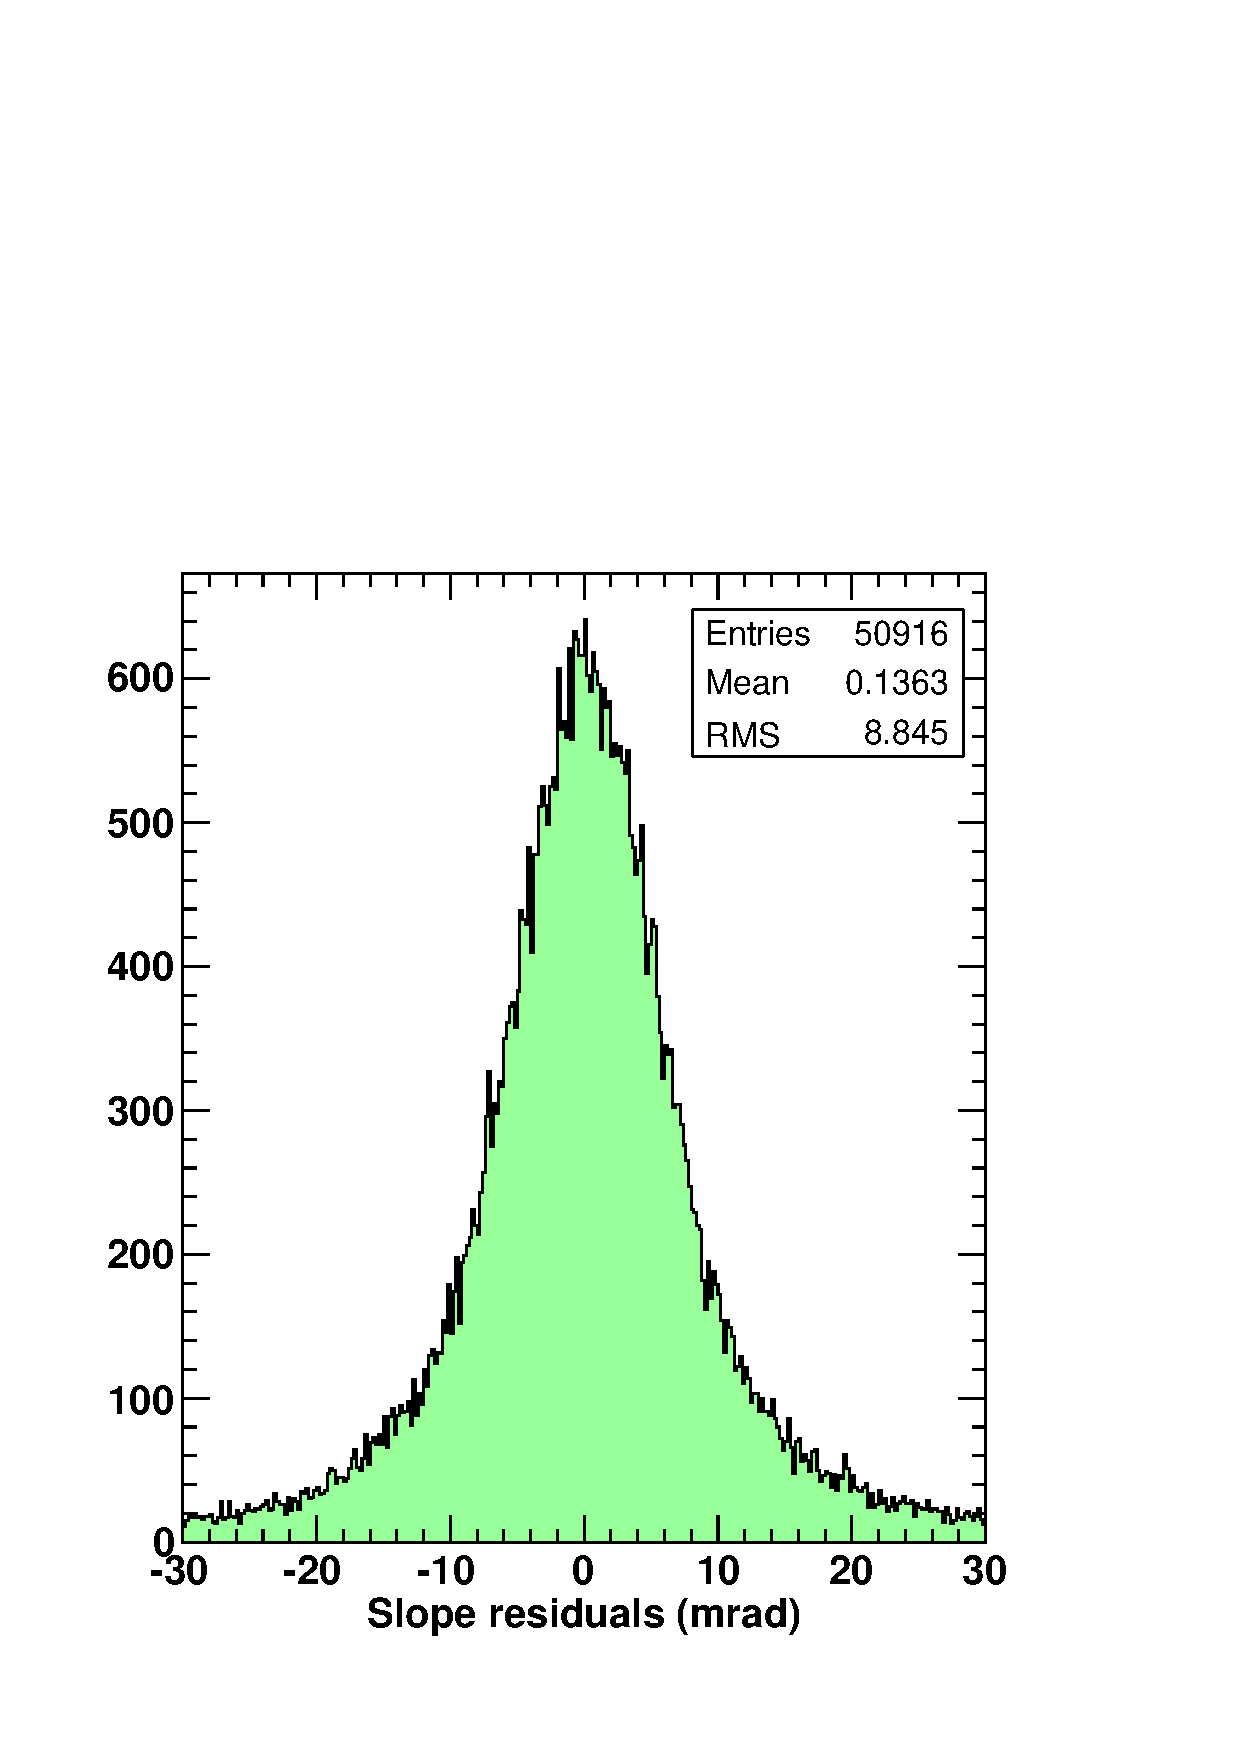
\includegraphics[width=0.35\linewidth]{slopeResiduals_badphiy.pdf}\hspace{1 cm}
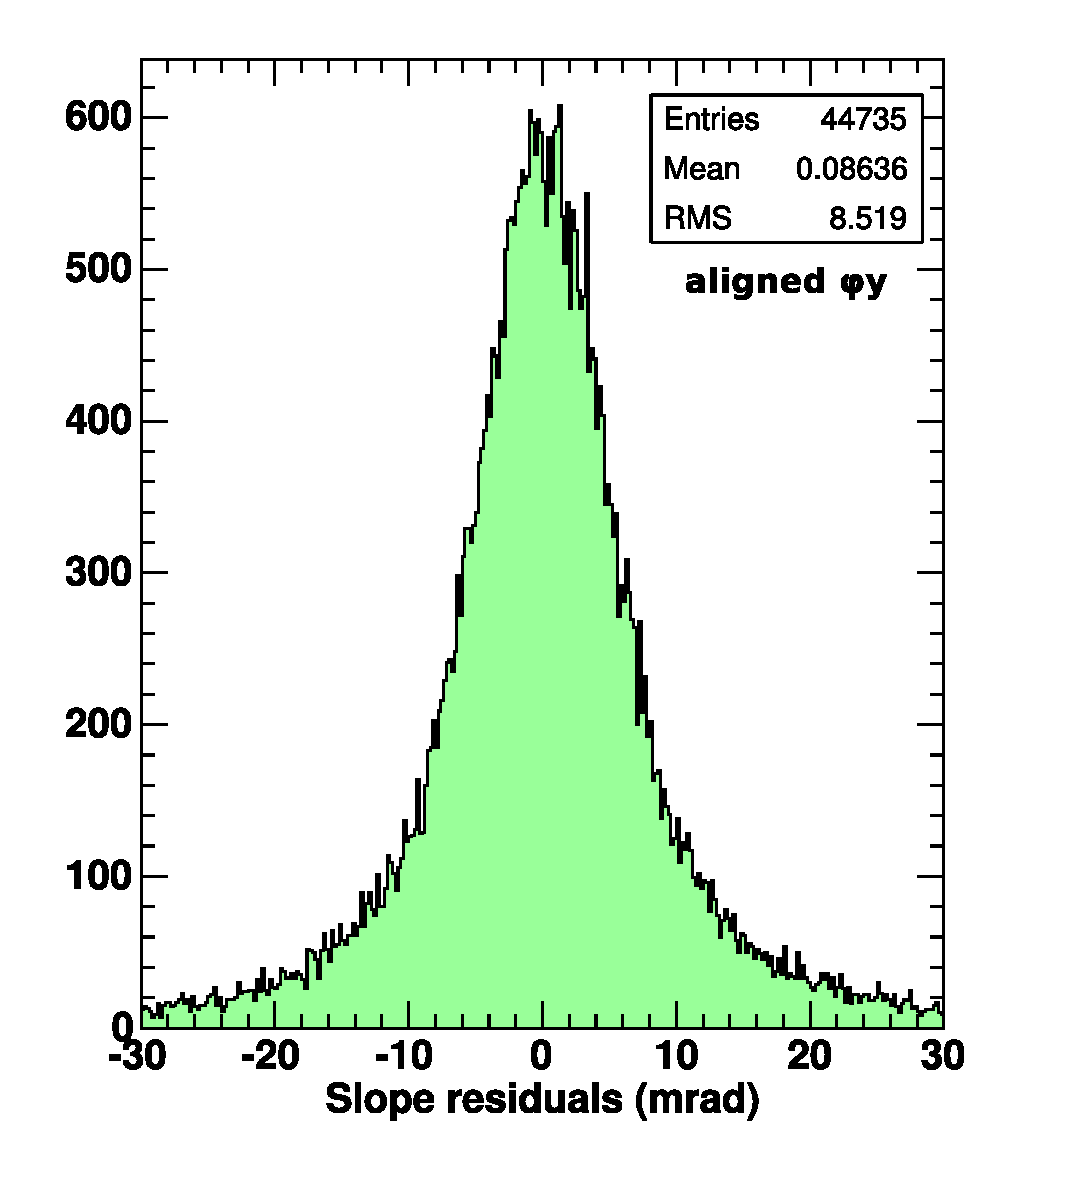
\includegraphics[width=0.35\linewidth]{slopeResiduals_goodphiy.pdf}
\end{center}

\caption{Offset residuals without (top-left) and with (top-right)
  $\phi_y$ pre-alignment, and slope residuals without (bottom-left)
  and with (bottom-right) $\phi_y$
  pre-alignment. \label{fig:offsetResiduals_badphiy}}
\end{figure}

\subsection{Other details of the method}

Hit weights were used to fit track-segments, but no weighting was used
to determine the average offset residual in each overlap--- only a
truncated mean.  Only overlaps with ten or more muons were used to
constrain the alignment, and uncertainties in offset-residuals means
were calculated as $\mbox{RMS}/\sqrt{N_\s{overlap muons}}$.

Coordinates were individually aligned in several passes.  The first
pass adjusted the radius of each ring such that the sum of all
overlap-residuals means is zero.  The next four passes alternately
align $r\phi$ and $\phi_z$; for example, in the second pass, $A_i$ and
$A_j$ in Eqn.~\ref{eqn:minimizeme} represent $r\phi$ corrections,
while in the third pass, they represent $\phi_z$ corrections.  The
fourth and fifth passes over $r\phi$ and $\phi_z$ are just to verify
that the two parameters have converged: no large changes are observed
after the third pass.

\section{Results and comparison to old data}

The following alignments were performed:
\begin{itemize}
\item BH$+$PG alignment using data from Mar.~2010 TCT test (currently
  the official geometry in the database);
\item BH$+$PG under the same conditions as above, but using
  summer~2010 data;
\item summer~2010 alignment like the above but the new hardware
  $z$/$\phi_x$ values;
\item summer~2010 alignment like the above but also using the new
  $\phi_y$ pre-alignment from collisions;
\item BH-only summer~2010 alignment with no input from PG (yet
  otherwise like the above);
\item BH$+$PG-only-in-gaps alignment: PG data were only used where BH
  overlaps do not exist.
\end{itemize}
Each subsection compares the results from one of these geometries with
the previous.  Histograms of differences in $r\phi$ and $\phi_z$ are
presented first, followed by differences versus chamber number for the
rings with the largest deviations, to look for a pattern.  In cases in
which differences are negligible (much less than 1~mm or 1~mrad),
only the histogram is shown.

Chambers are classified in three groups: ME1/1, inner (ME1/2 and
ME$x$/1), and outer (ME$x$/2), where $x \ge 2$.  Chambers within each
of these groups are affected by different considerations: ME1/1 have
no PG constraint, inner chambers have the highest beam-halo
statistics, and outer chambers have lower beam-halo statistics.  Three
histograms will therefore be filled in each study, one for each class
of chambers.

\subsection{Comparison of March (TCT) results with summer results}

The Mar.~2010 TCT run was a special run of the LHC designed to produce
high rates of beam-halo.  Both LHC beams were completely converted
into beam-halo muons in 40~minutes.  This provided a pure sample of
beam-halo used early in the year to produce an initial CSC geometry,
and it is still the official chambers-within-ring geometry used for
CMSSW reconstruction.  The summer~2010 data were collected over a
longer time period during collisions data-taking.  We do not expect
significant motion of the chambers between March and the summer, and
observed differences cannot be easily interpreted as physical motions
because of the changes in conditions (trigger, available BH overlaps,
and slightly tighter $|dr/dz|$ window: see
Figs.~\ref{fig:occupancy_March2010} and \ref{fig:drdz_Dec2009}).

Figure~\ref{fig:TCTtoCollisions_histograms} presents differences
between the March alignment and the summer alignment.  The largest
differences are in ME1/1 and can be attributed to new overlap
measurements that were not available in March (especially in
ME$+$1/1).  A group of chambers in ME$+$1/1 between 7 and 30 (inclusive)
rotated around the beamline by 1~mm with respect to the others: this
region is bordered by two overlaps measurements that were not
available in March but now are (see
Fig.~\ref{fig:occupancy_March2010}).  Outer chambers have larger
differences between the two datasets than inner chambers, but without
a clear pattern.

Figure~\ref{fig:TCTtoCollisions_phiz_histograms} shows the same for
$\phi_z$, which has structures bordered by missing BH data, just as in
$r\phi$.  Differences in all other rings are completely negligible.

\begin{figure}
\begin{center}
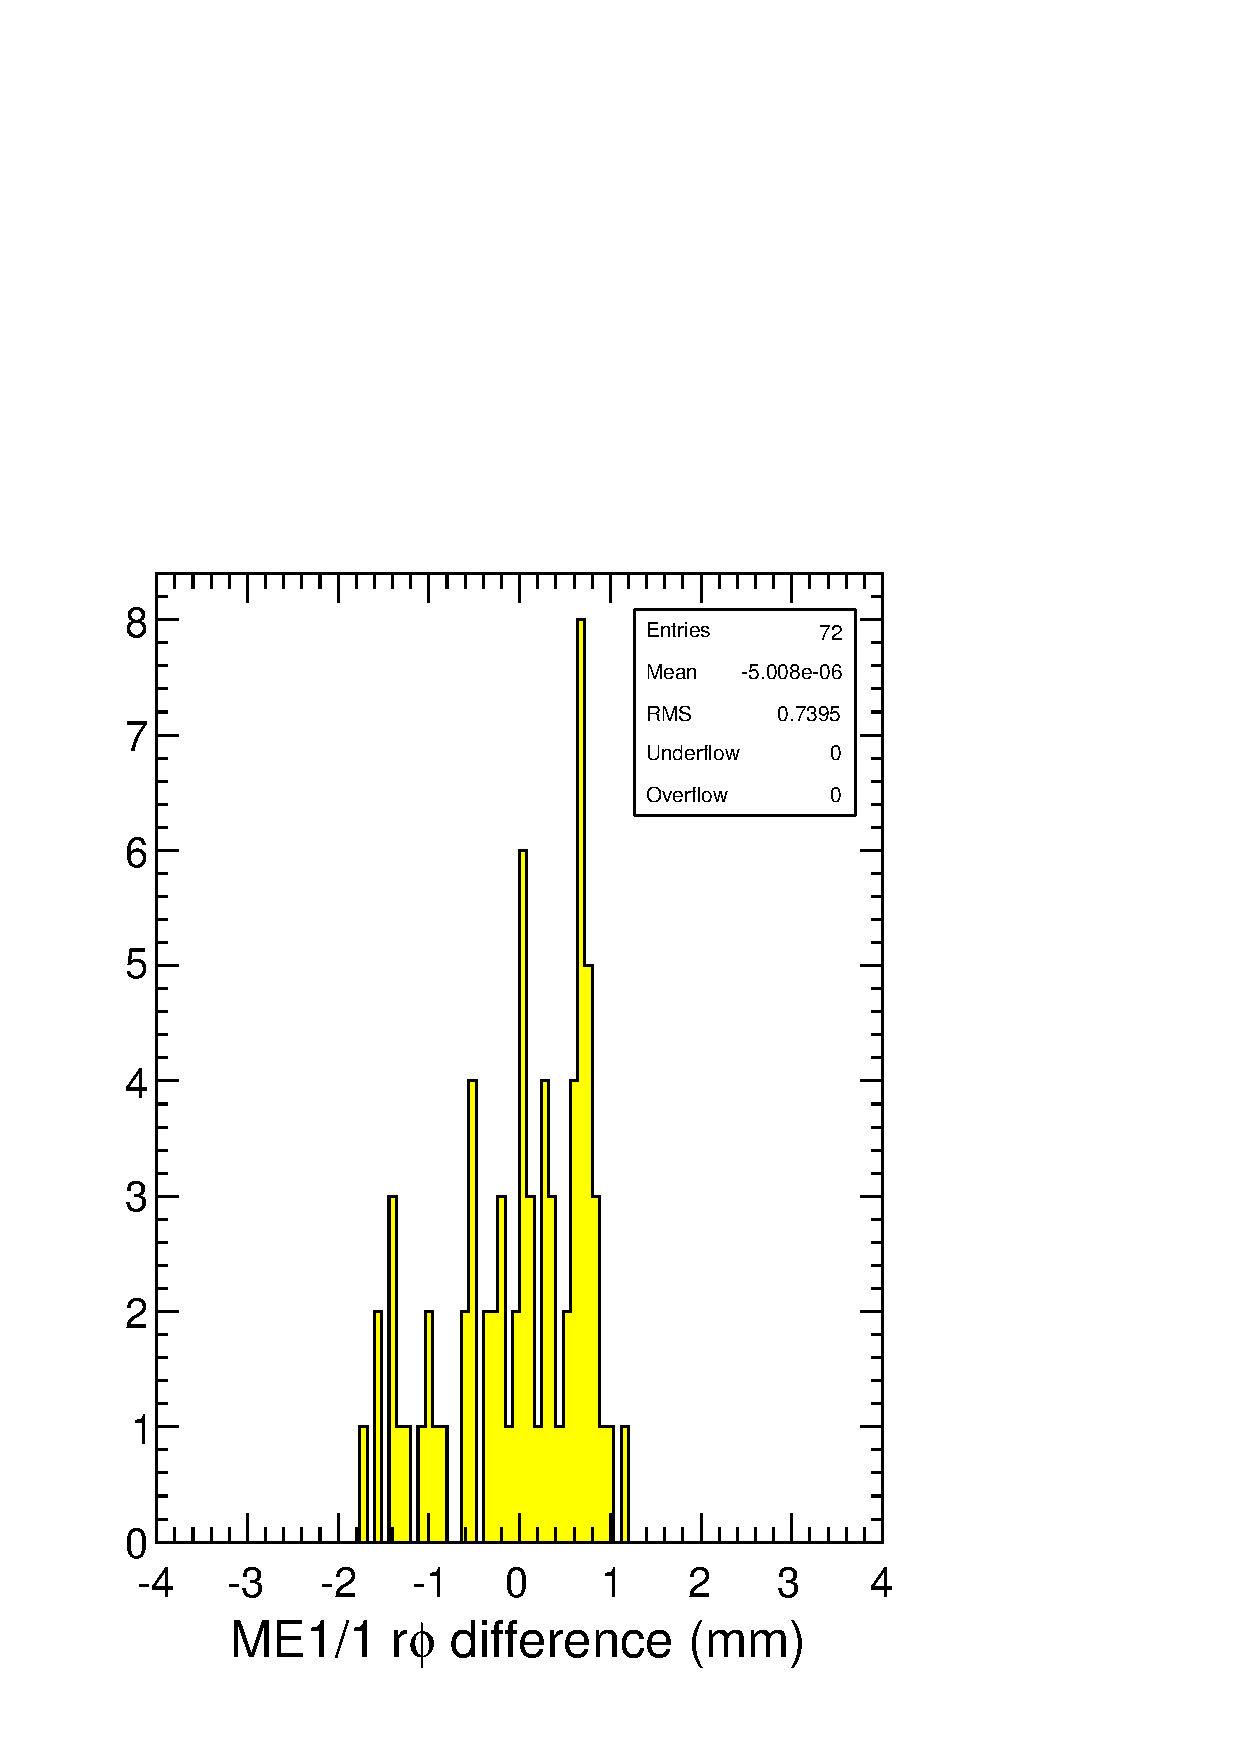
\includegraphics[width=0.32\linewidth]{TCTtoCollisions_me11.pdf}
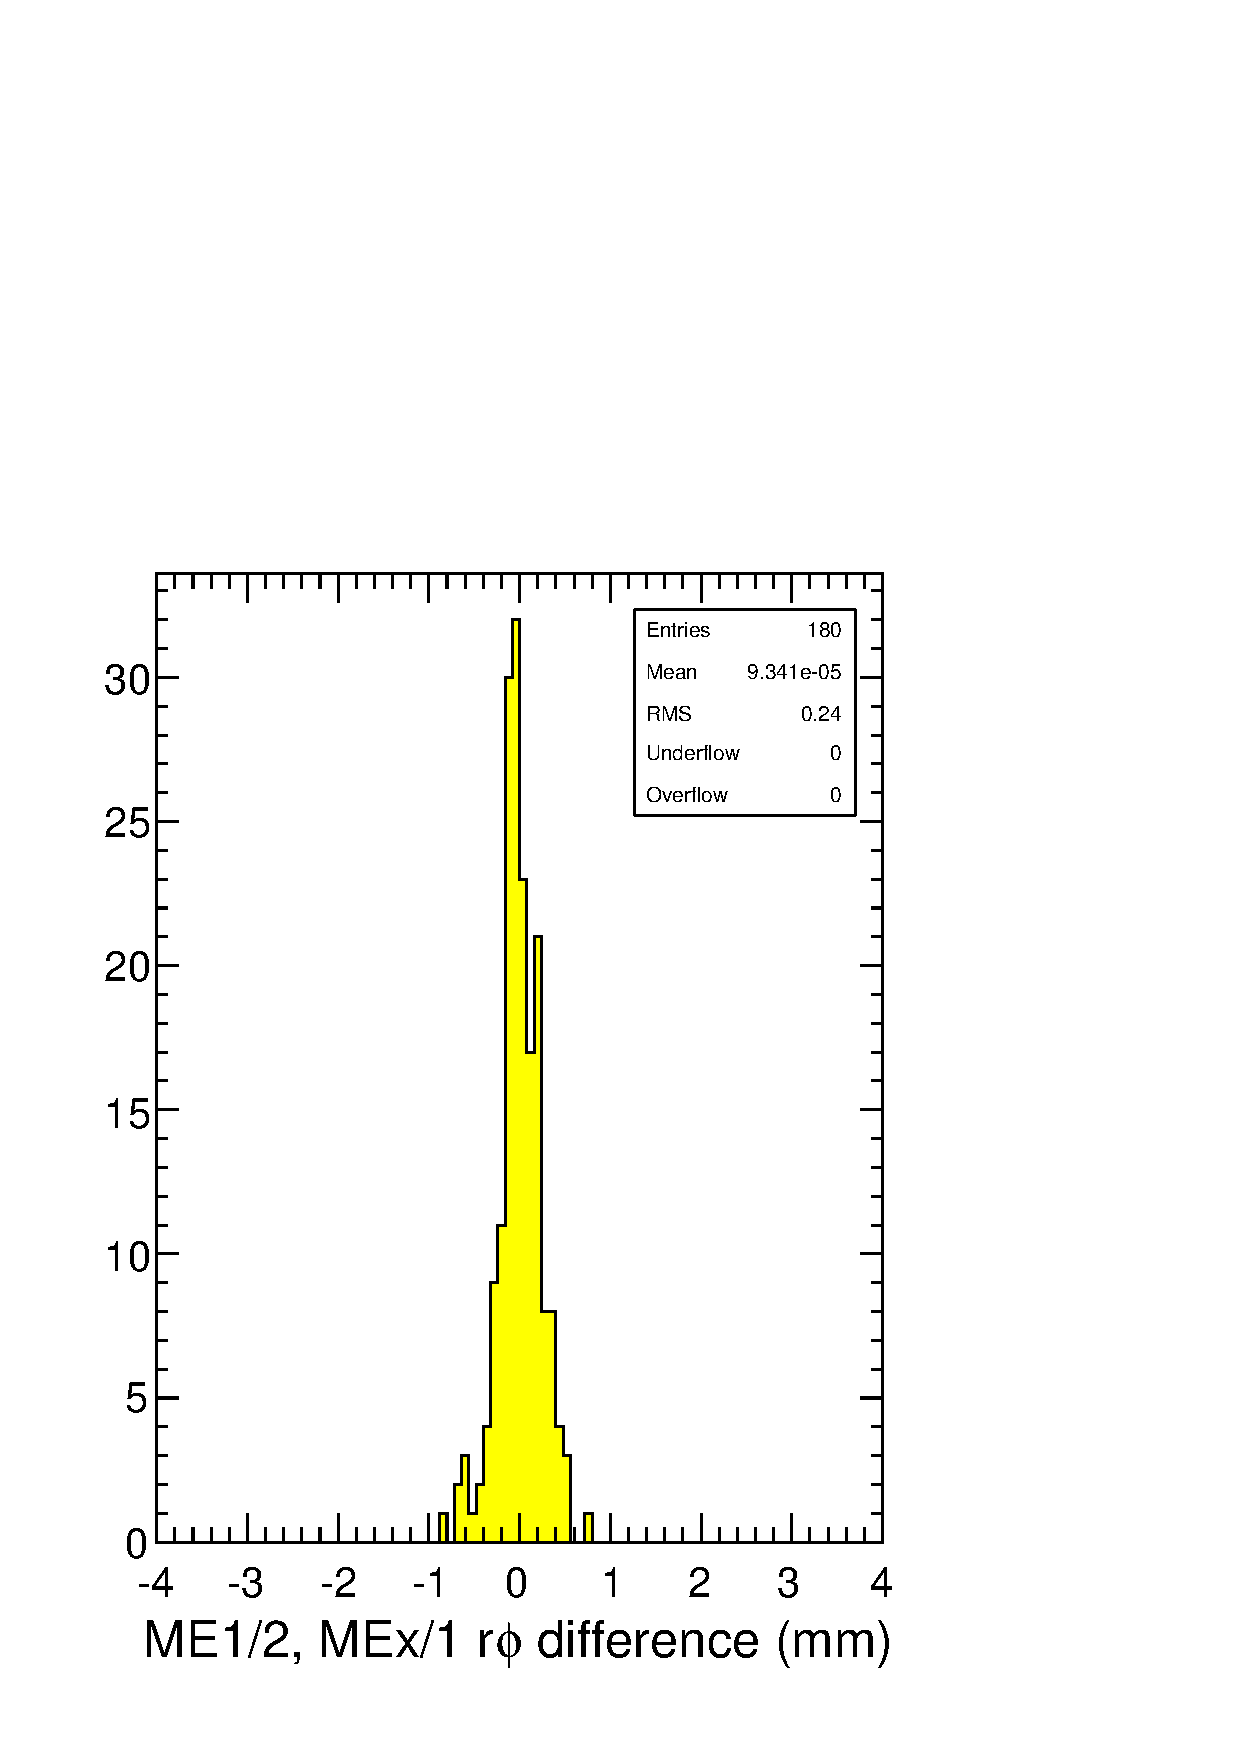
\includegraphics[width=0.32\linewidth]{TCTtoCollisions_inner.pdf}
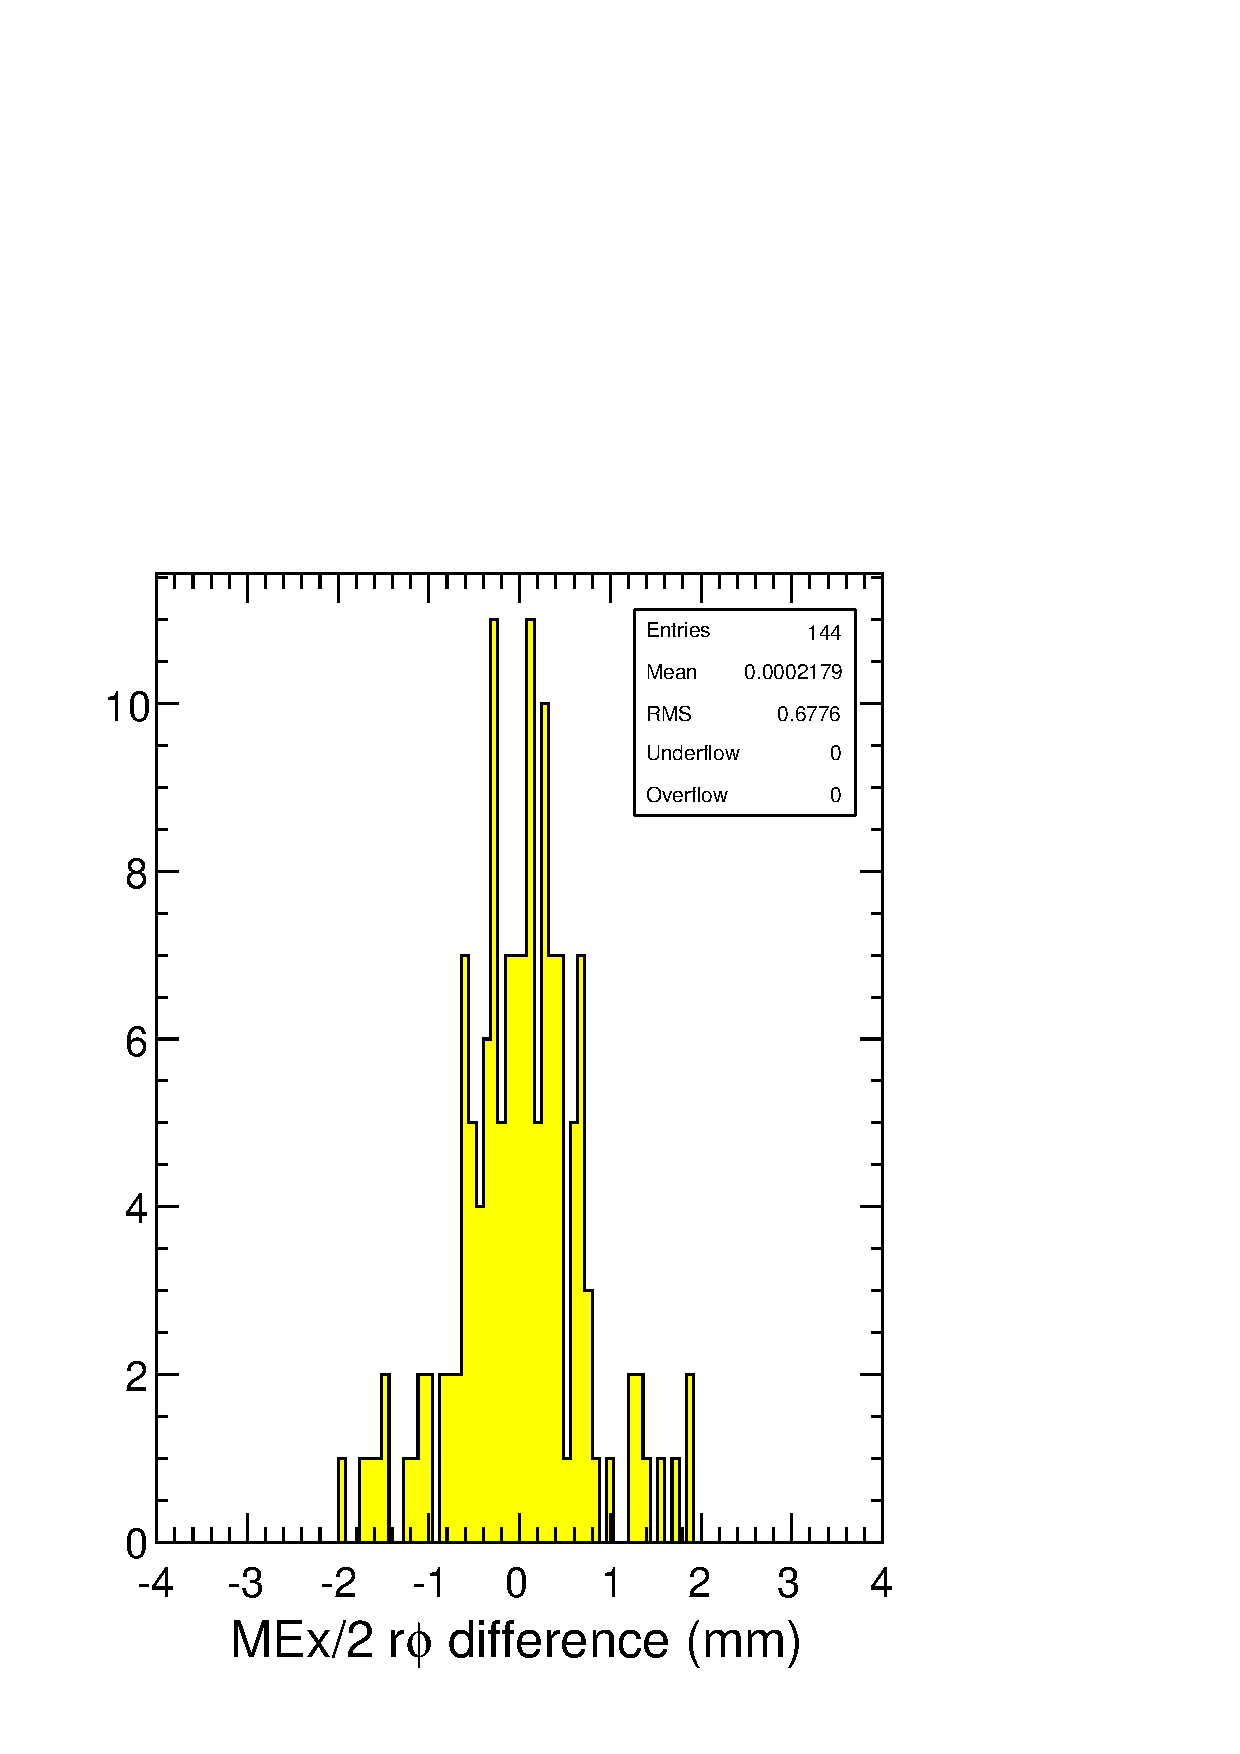
\includegraphics[width=0.32\linewidth]{TCTtoCollisions_outer.pdf}

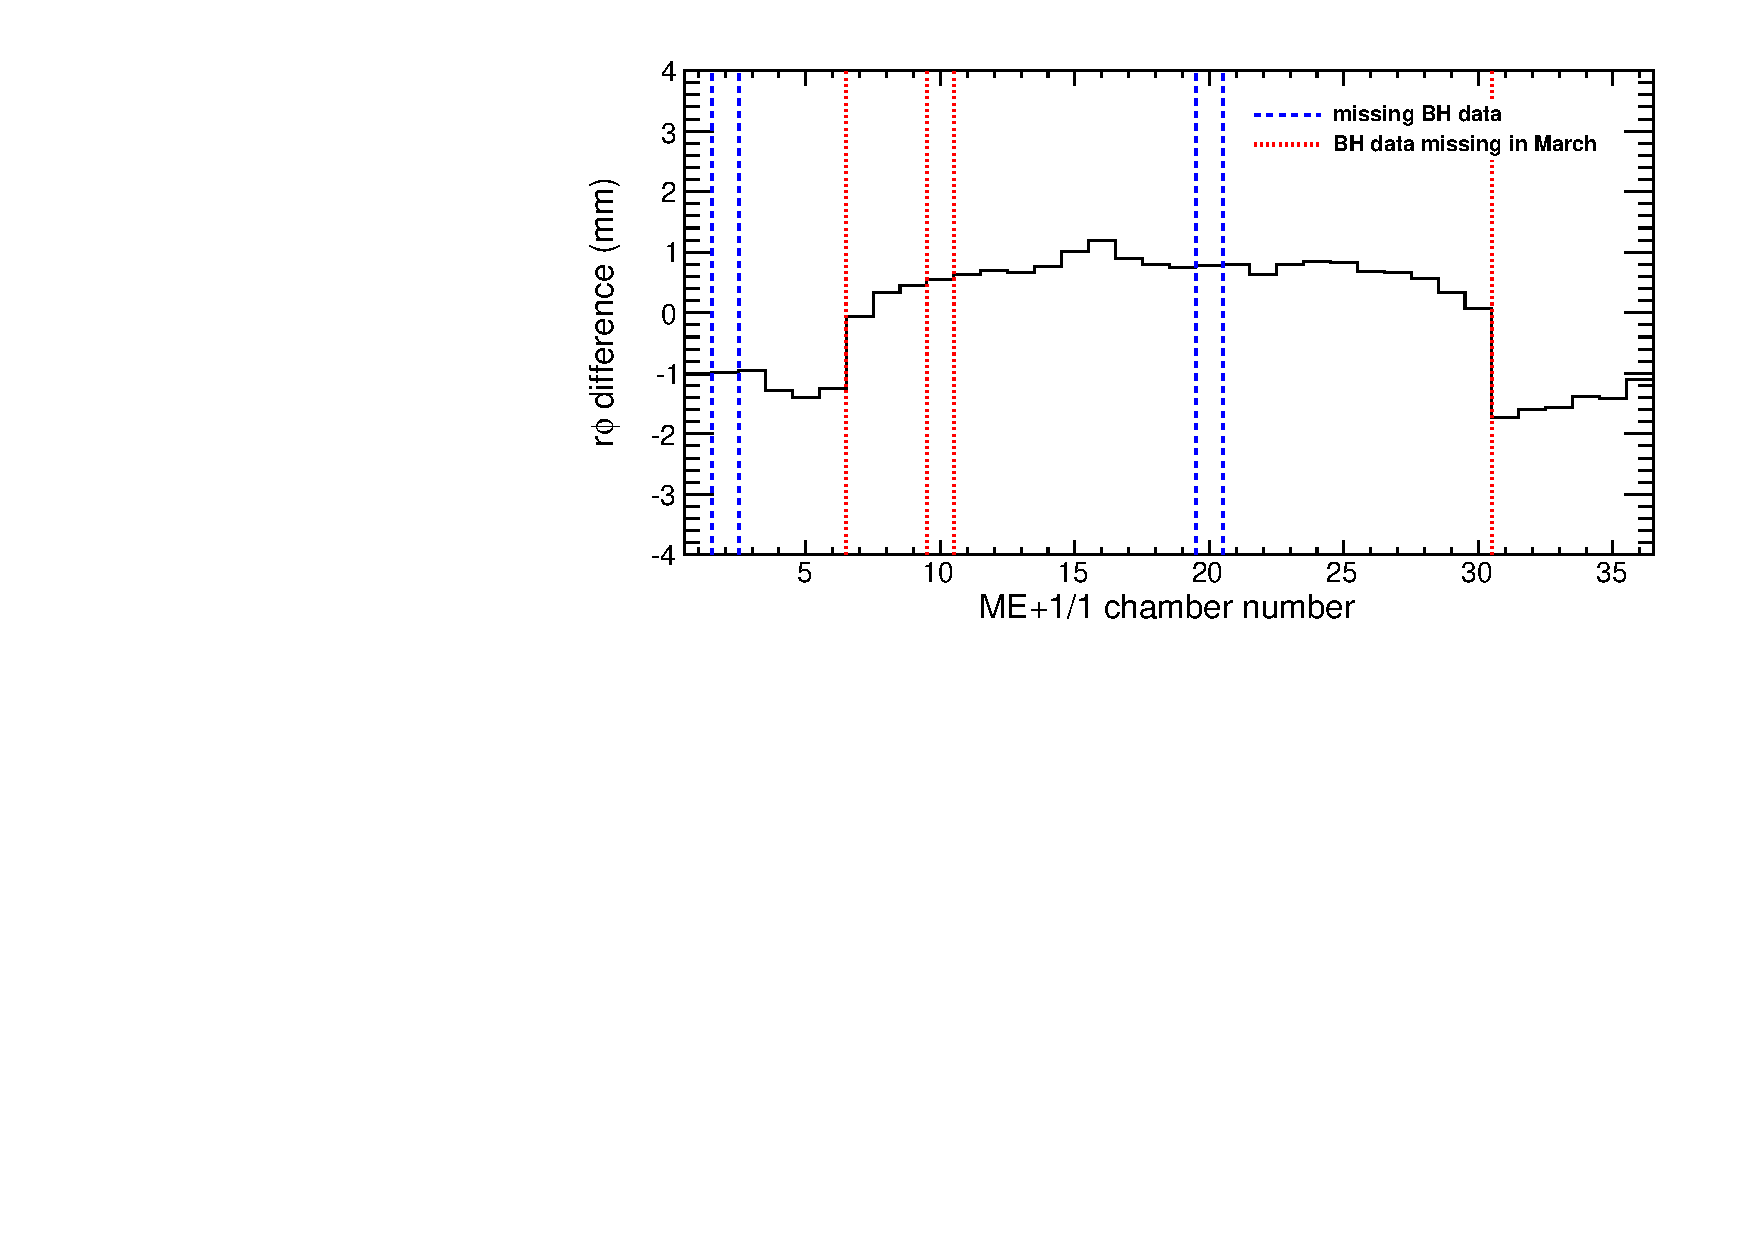
\includegraphics[width=0.45\linewidth]{TCTtoCollisions_mep11.pdf}
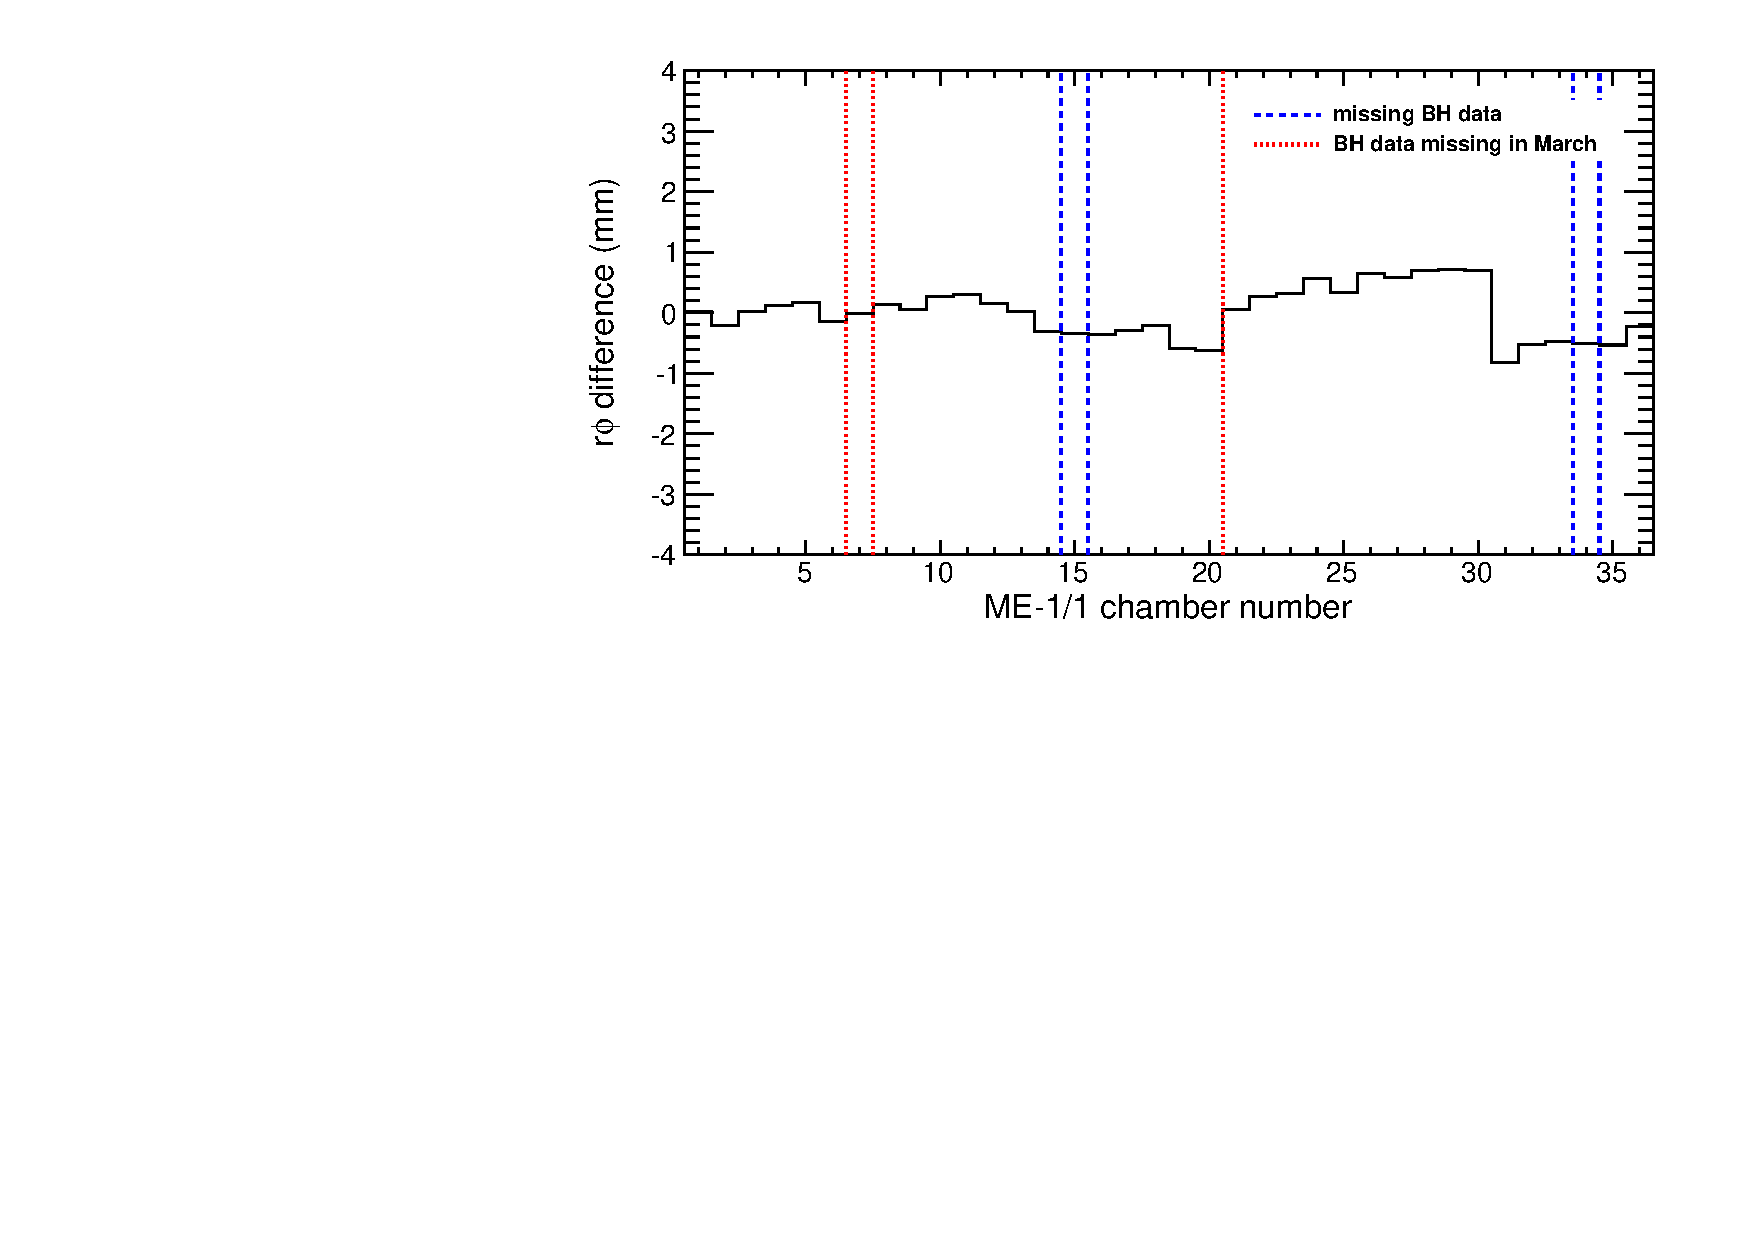
\includegraphics[width=0.45\linewidth]{TCTtoCollisions_mem11.pdf}

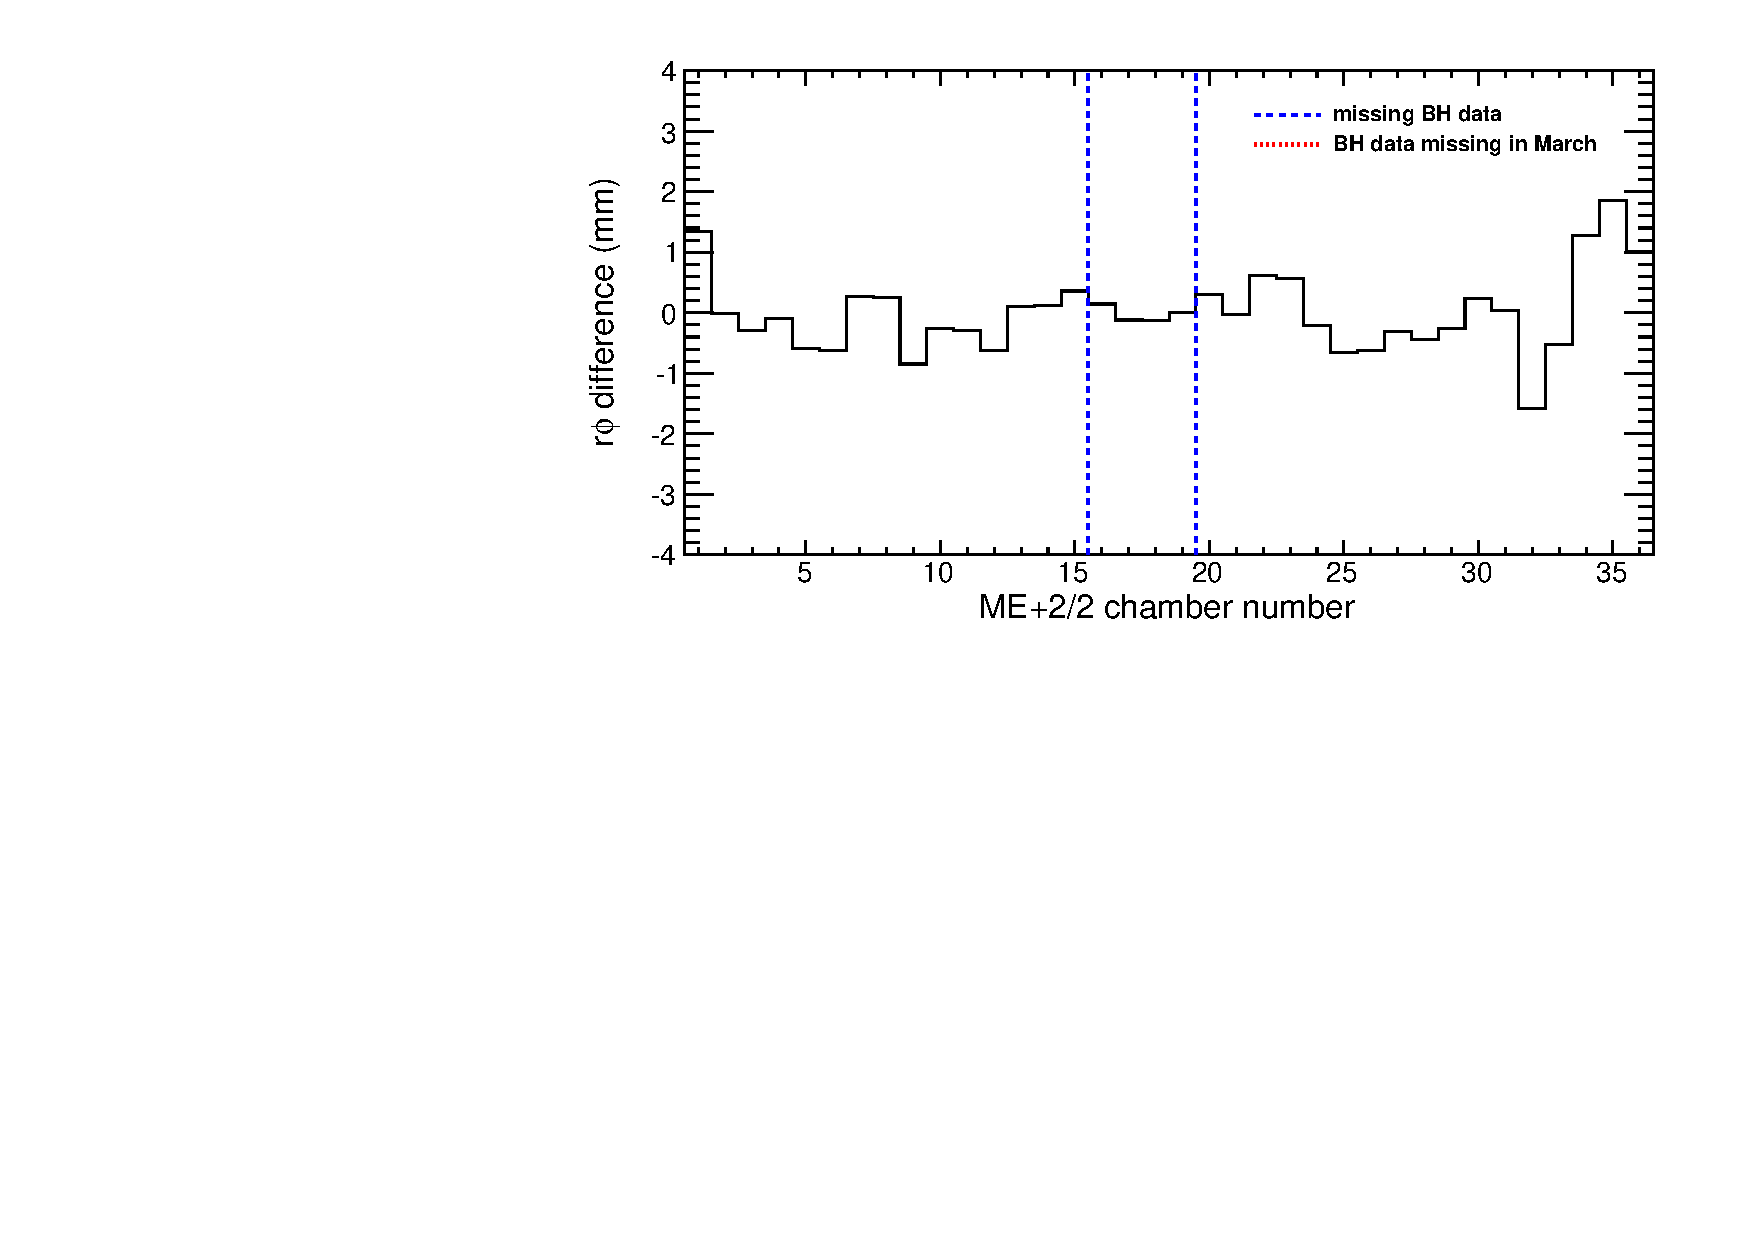
\includegraphics[width=0.45\linewidth]{TCTtoCollisions_mep22.pdf}
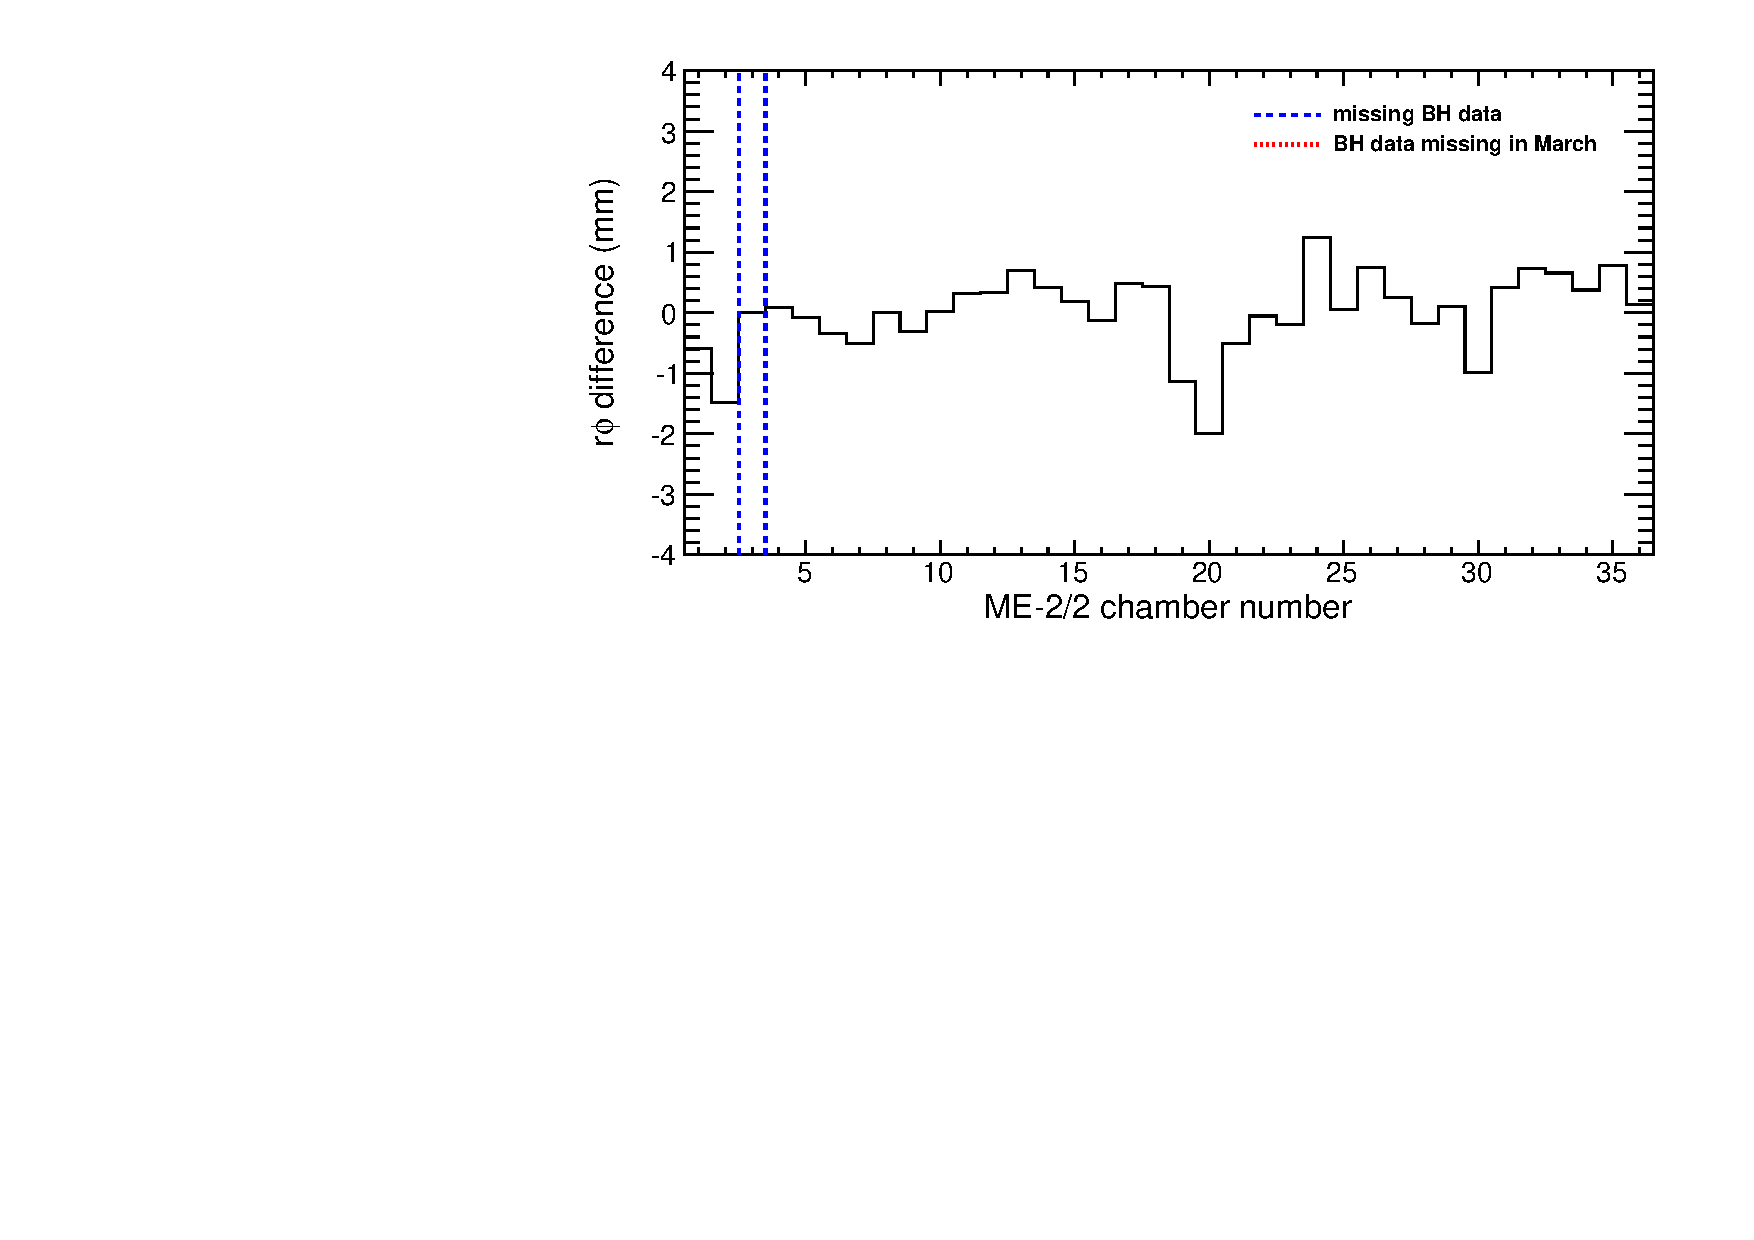
\includegraphics[width=0.45\linewidth]{TCTtoCollisions_mem22.pdf}

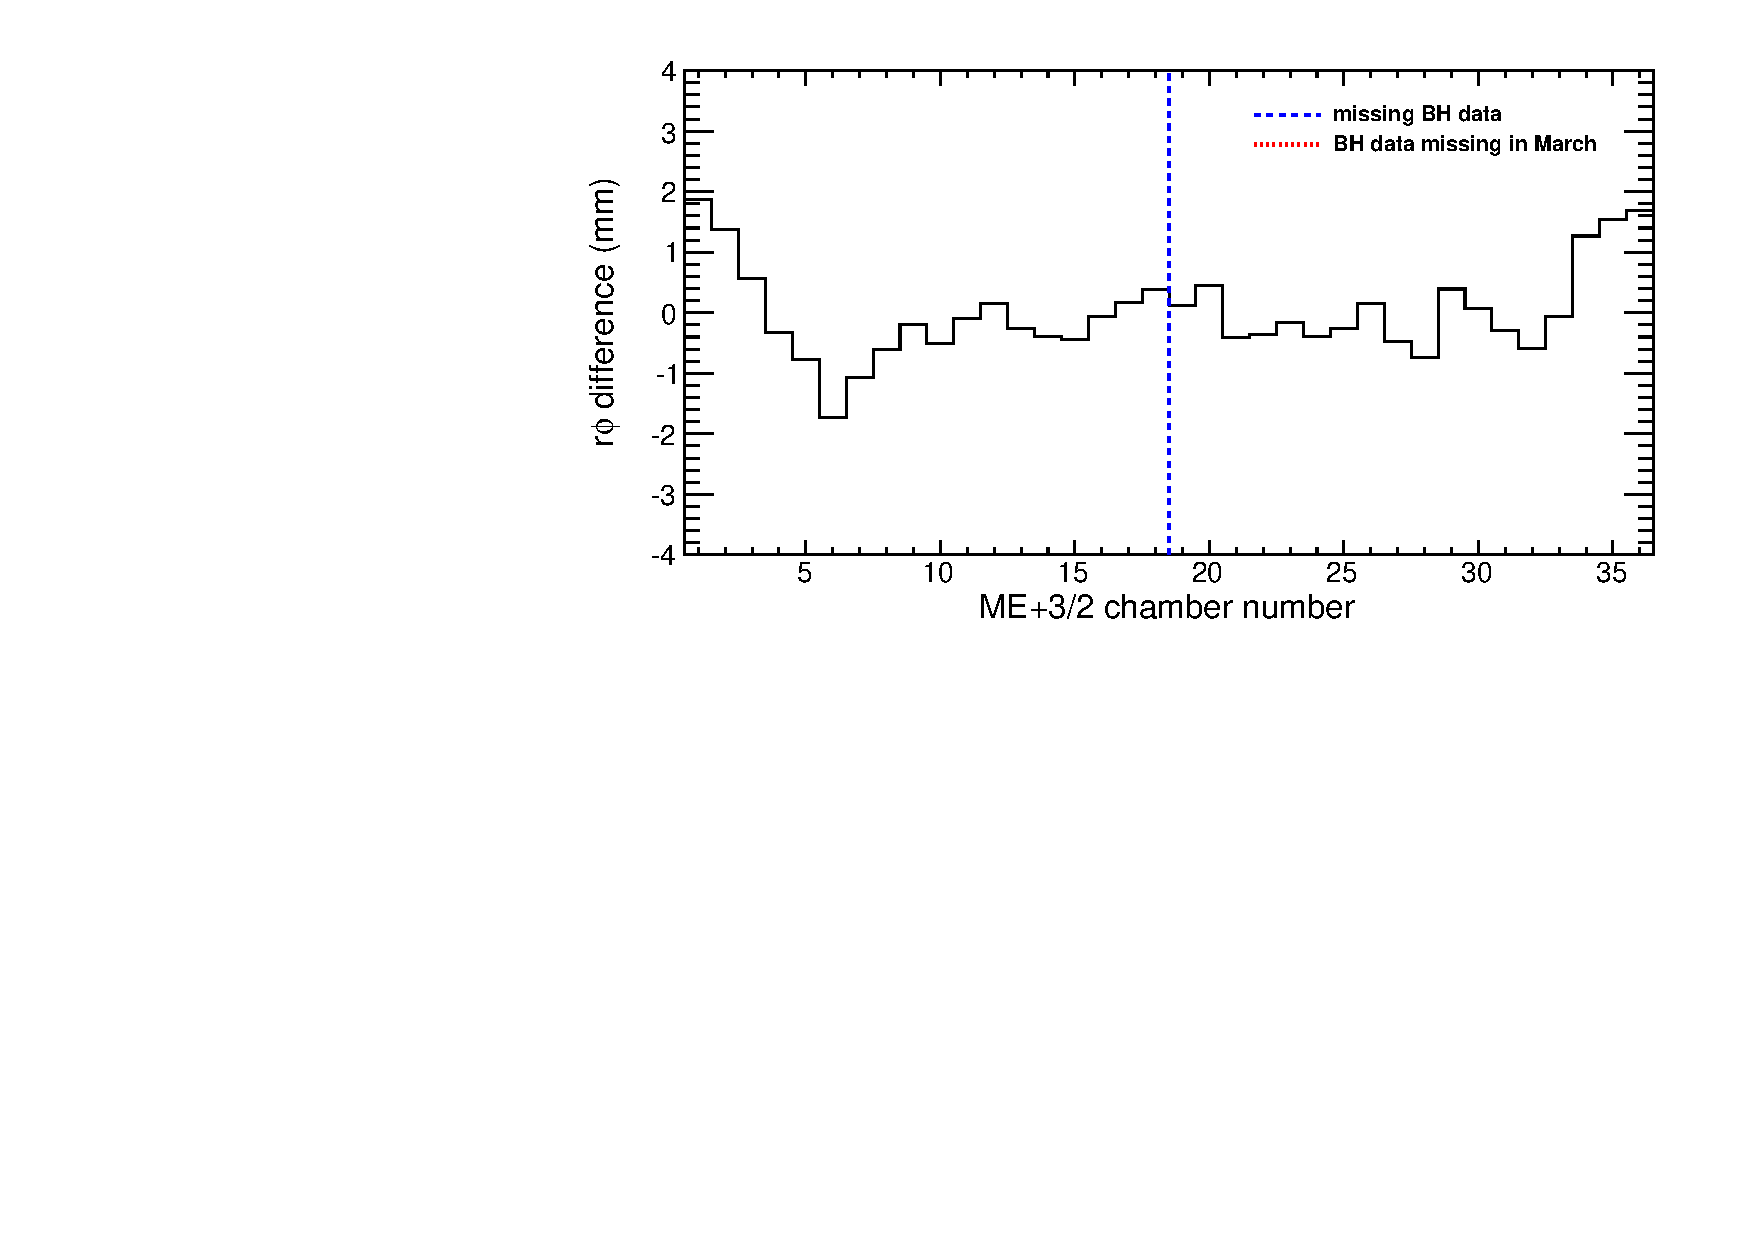
\includegraphics[width=0.45\linewidth]{TCTtoCollisions_mep32.pdf}
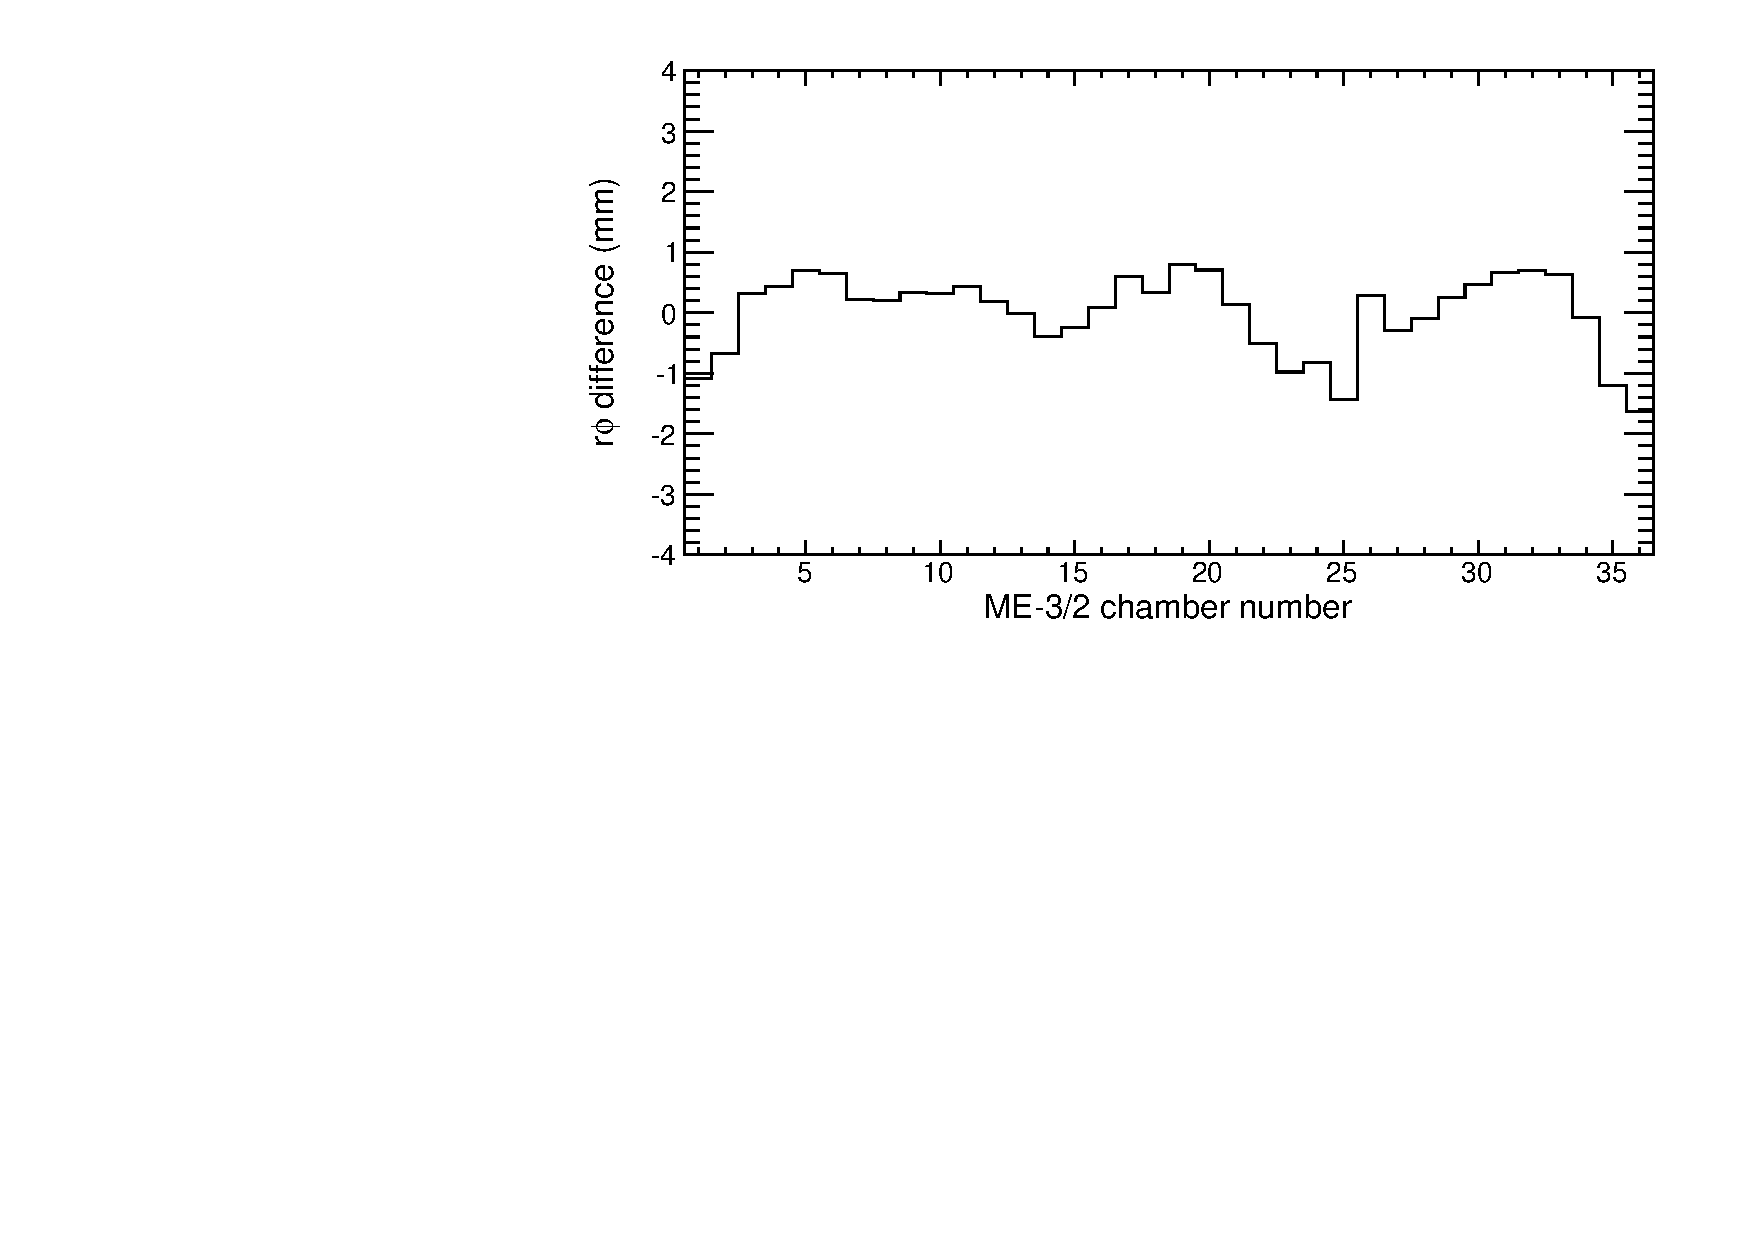
\includegraphics[width=0.45\linewidth]{TCTtoCollisions_mem32.pdf}
\end{center}

\caption{Differences in $r\phi$ parameters between the Mar.~2010 TCT
  alignment and the summer~2010 during-collisions alignment.  The
  largest differences are in ME$+$1/1, where two new overlaps
  measurements became available (6-7 and 30-31) and shifted
  everything in between them coherently.  No systematic changes in
  shape were observed in ME2/2 and 3/2, though the size of the
  changes are 0.6~mm (RMS). \label{fig:TCTtoCollisions_histograms}}
\end{figure}

\begin{figure}
\begin{center}
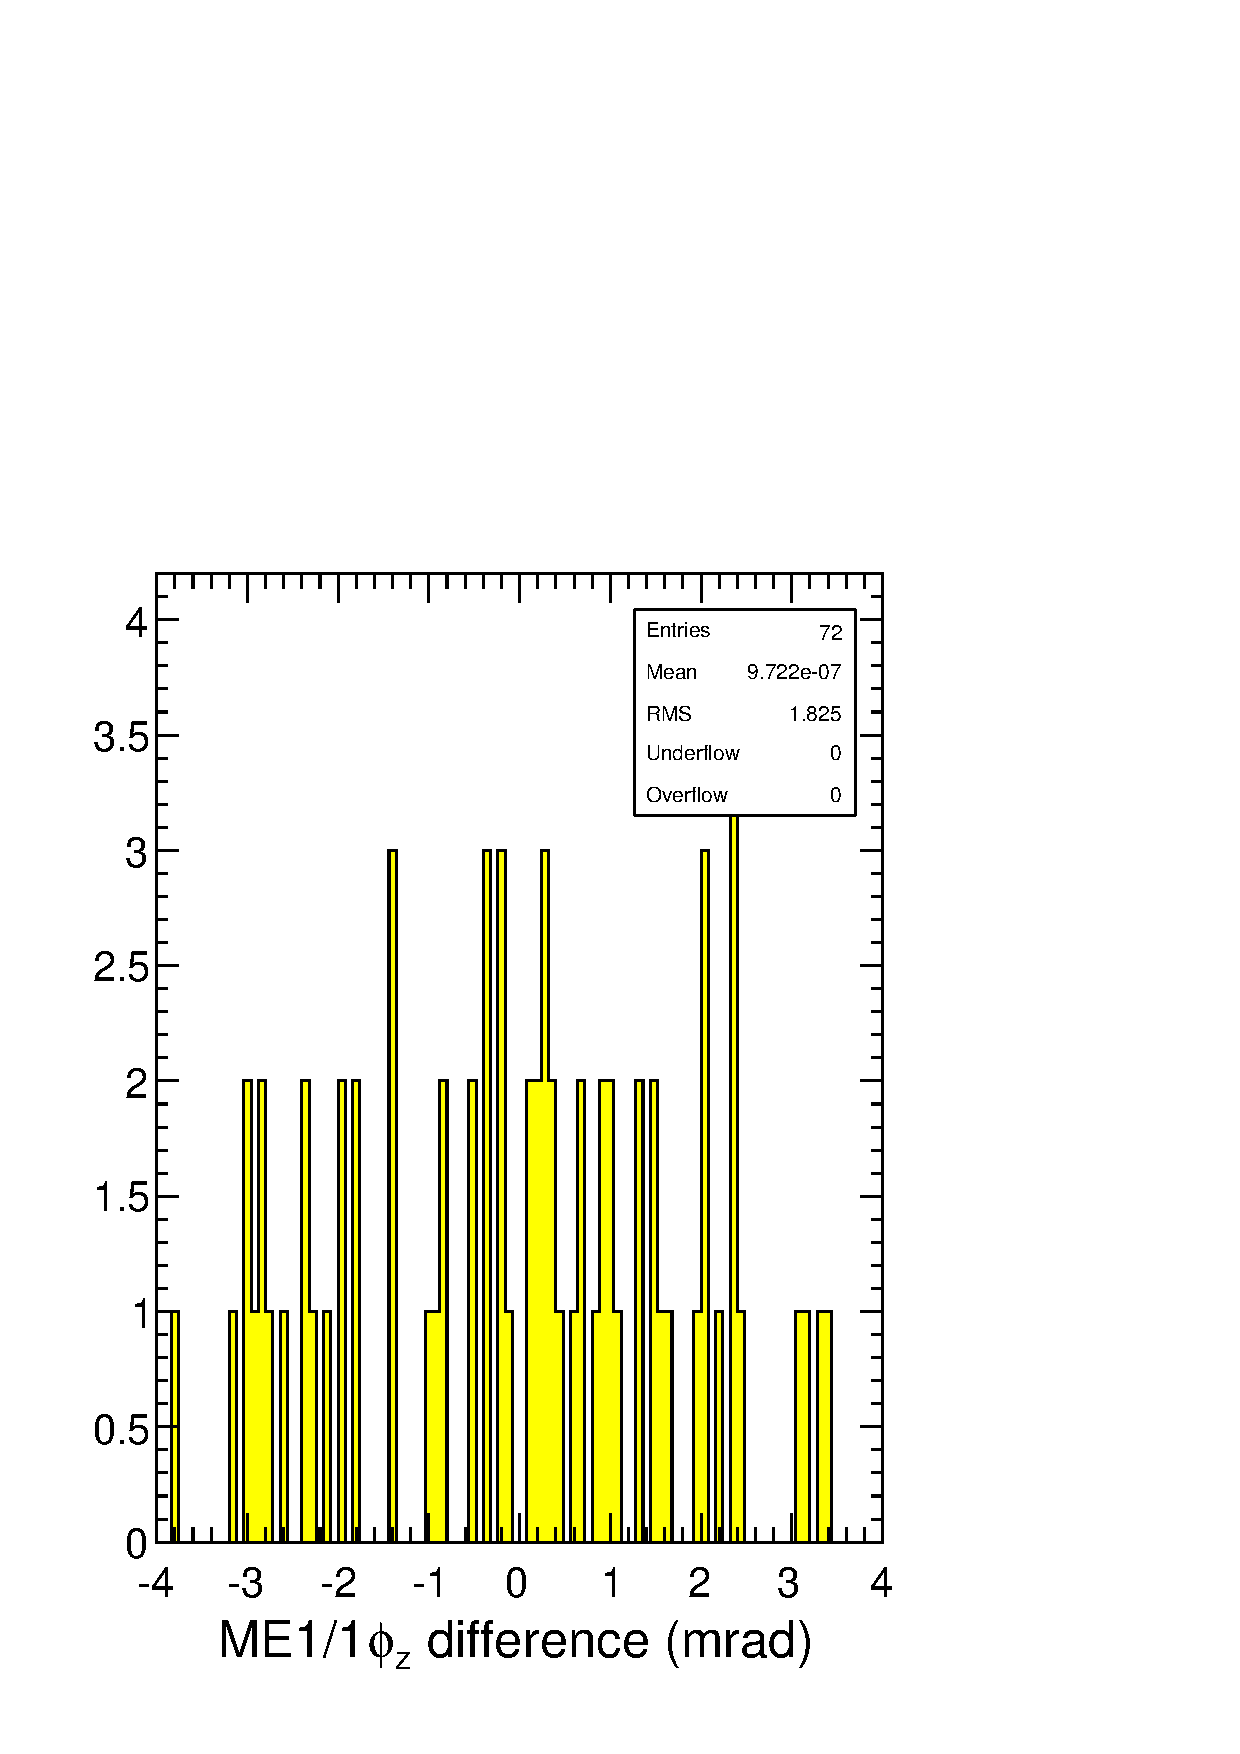
\includegraphics[width=0.32\linewidth]{TCTtoCollisions_phiz_me11.pdf}
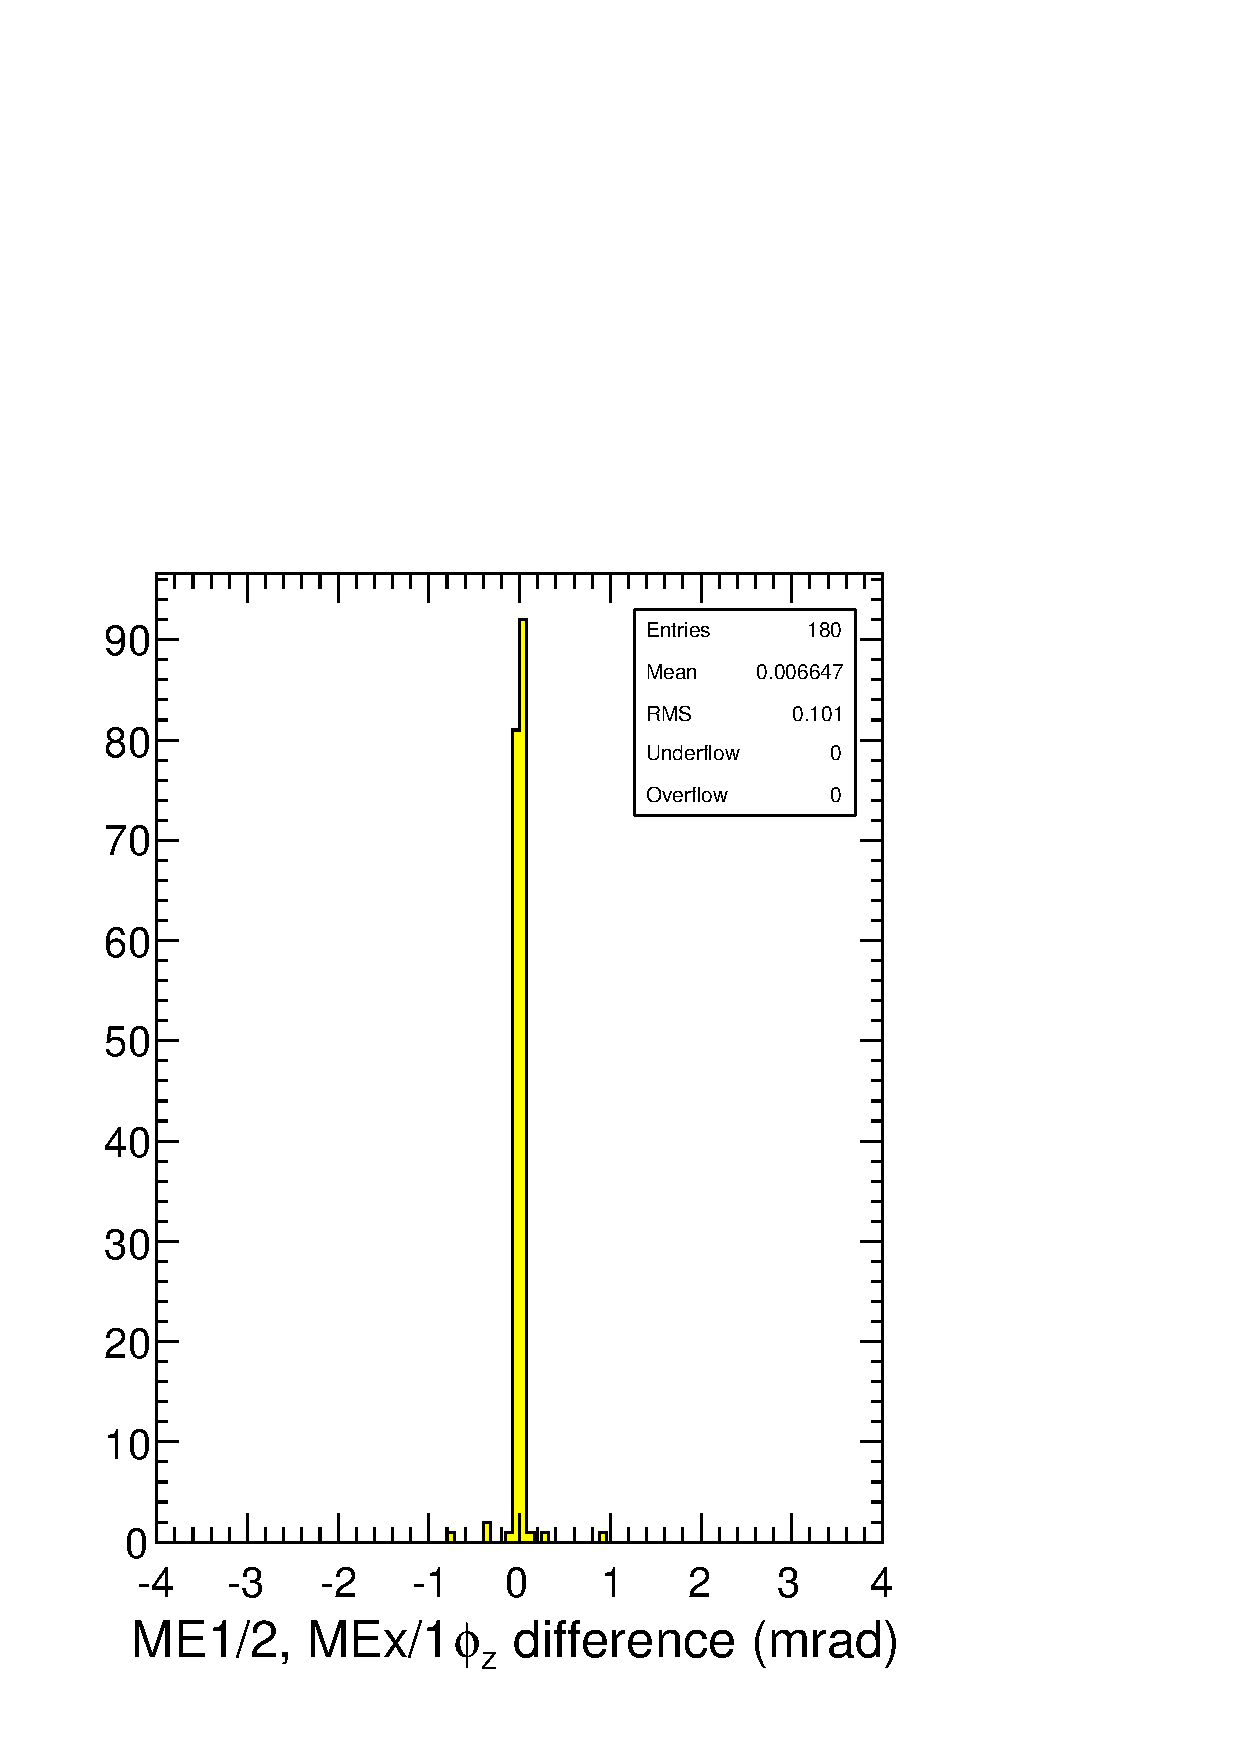
\includegraphics[width=0.32\linewidth]{TCTtoCollisions_phiz_inner.pdf}
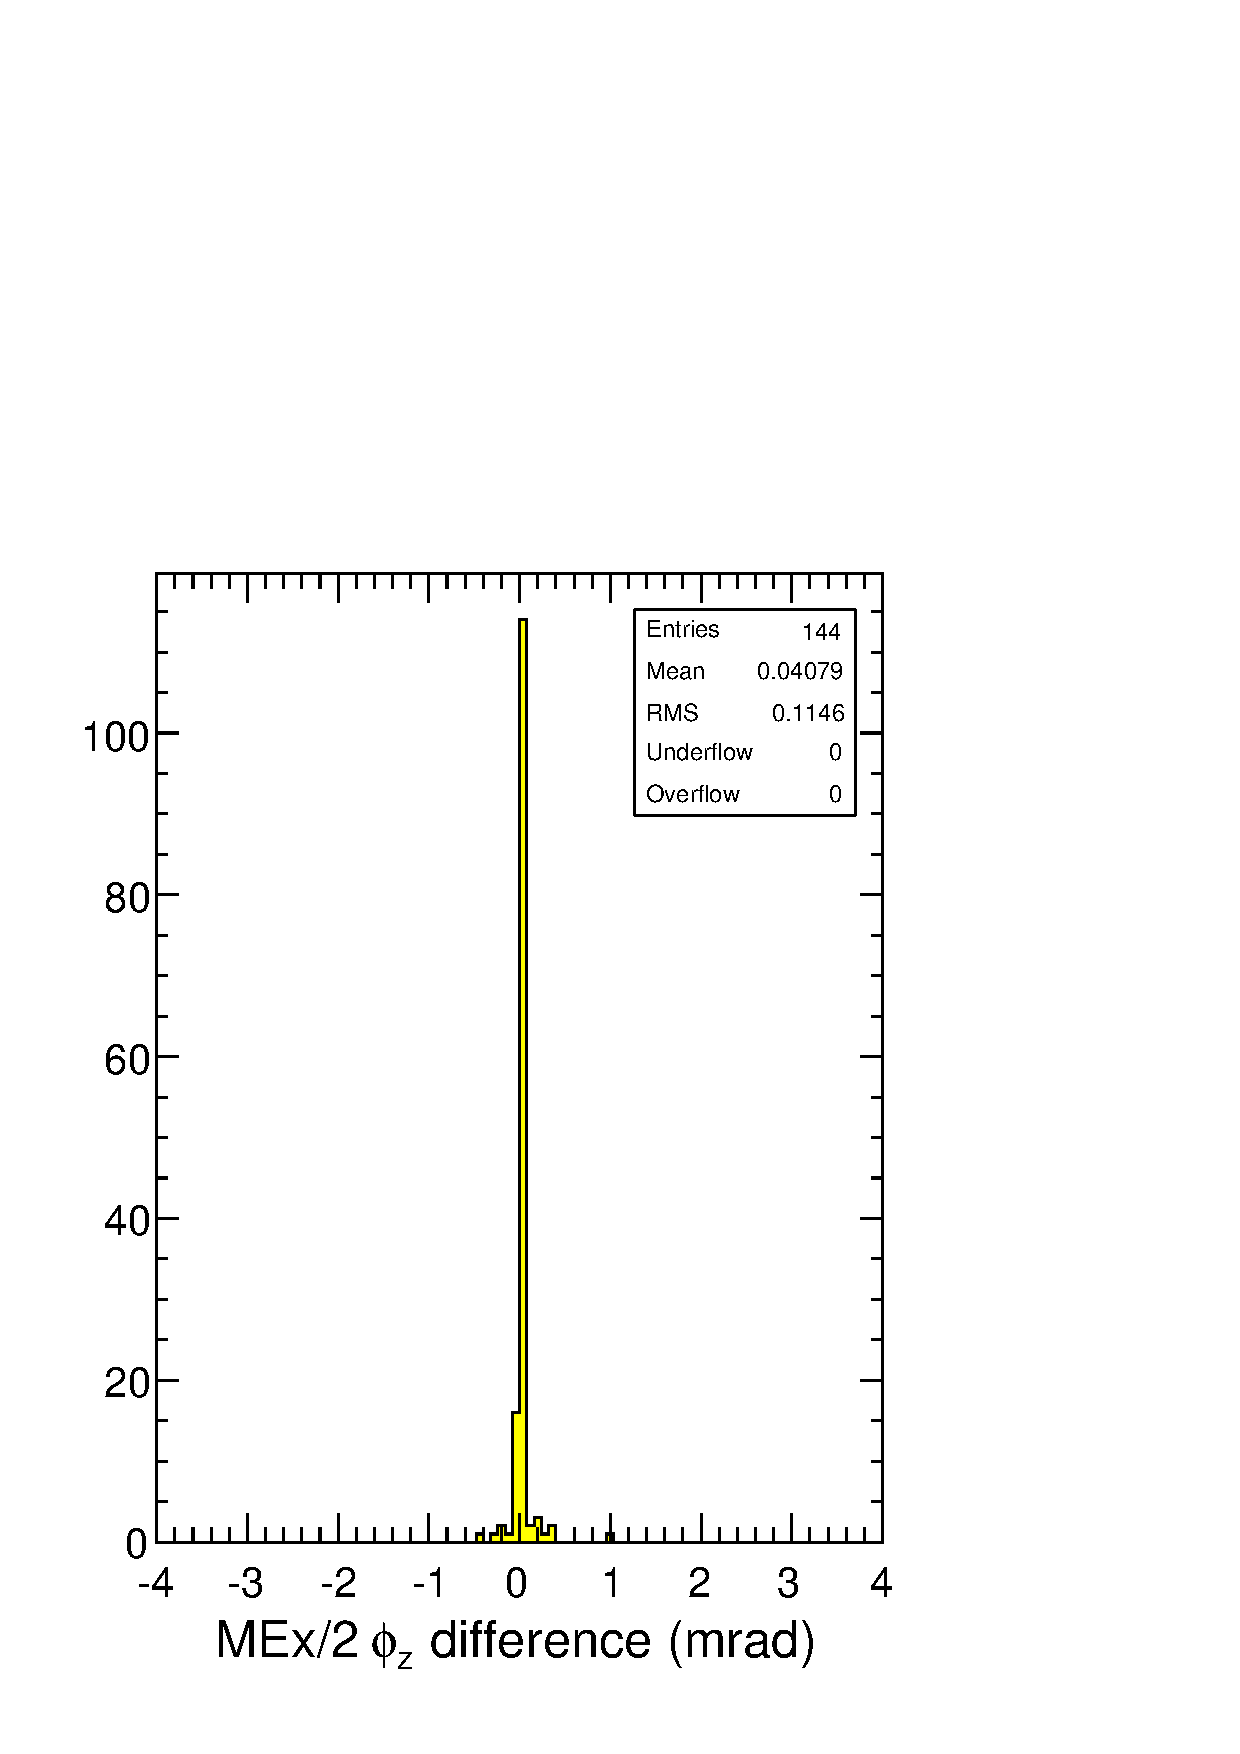
\includegraphics[width=0.32\linewidth]{TCTtoCollisions_phiz_outer.pdf}

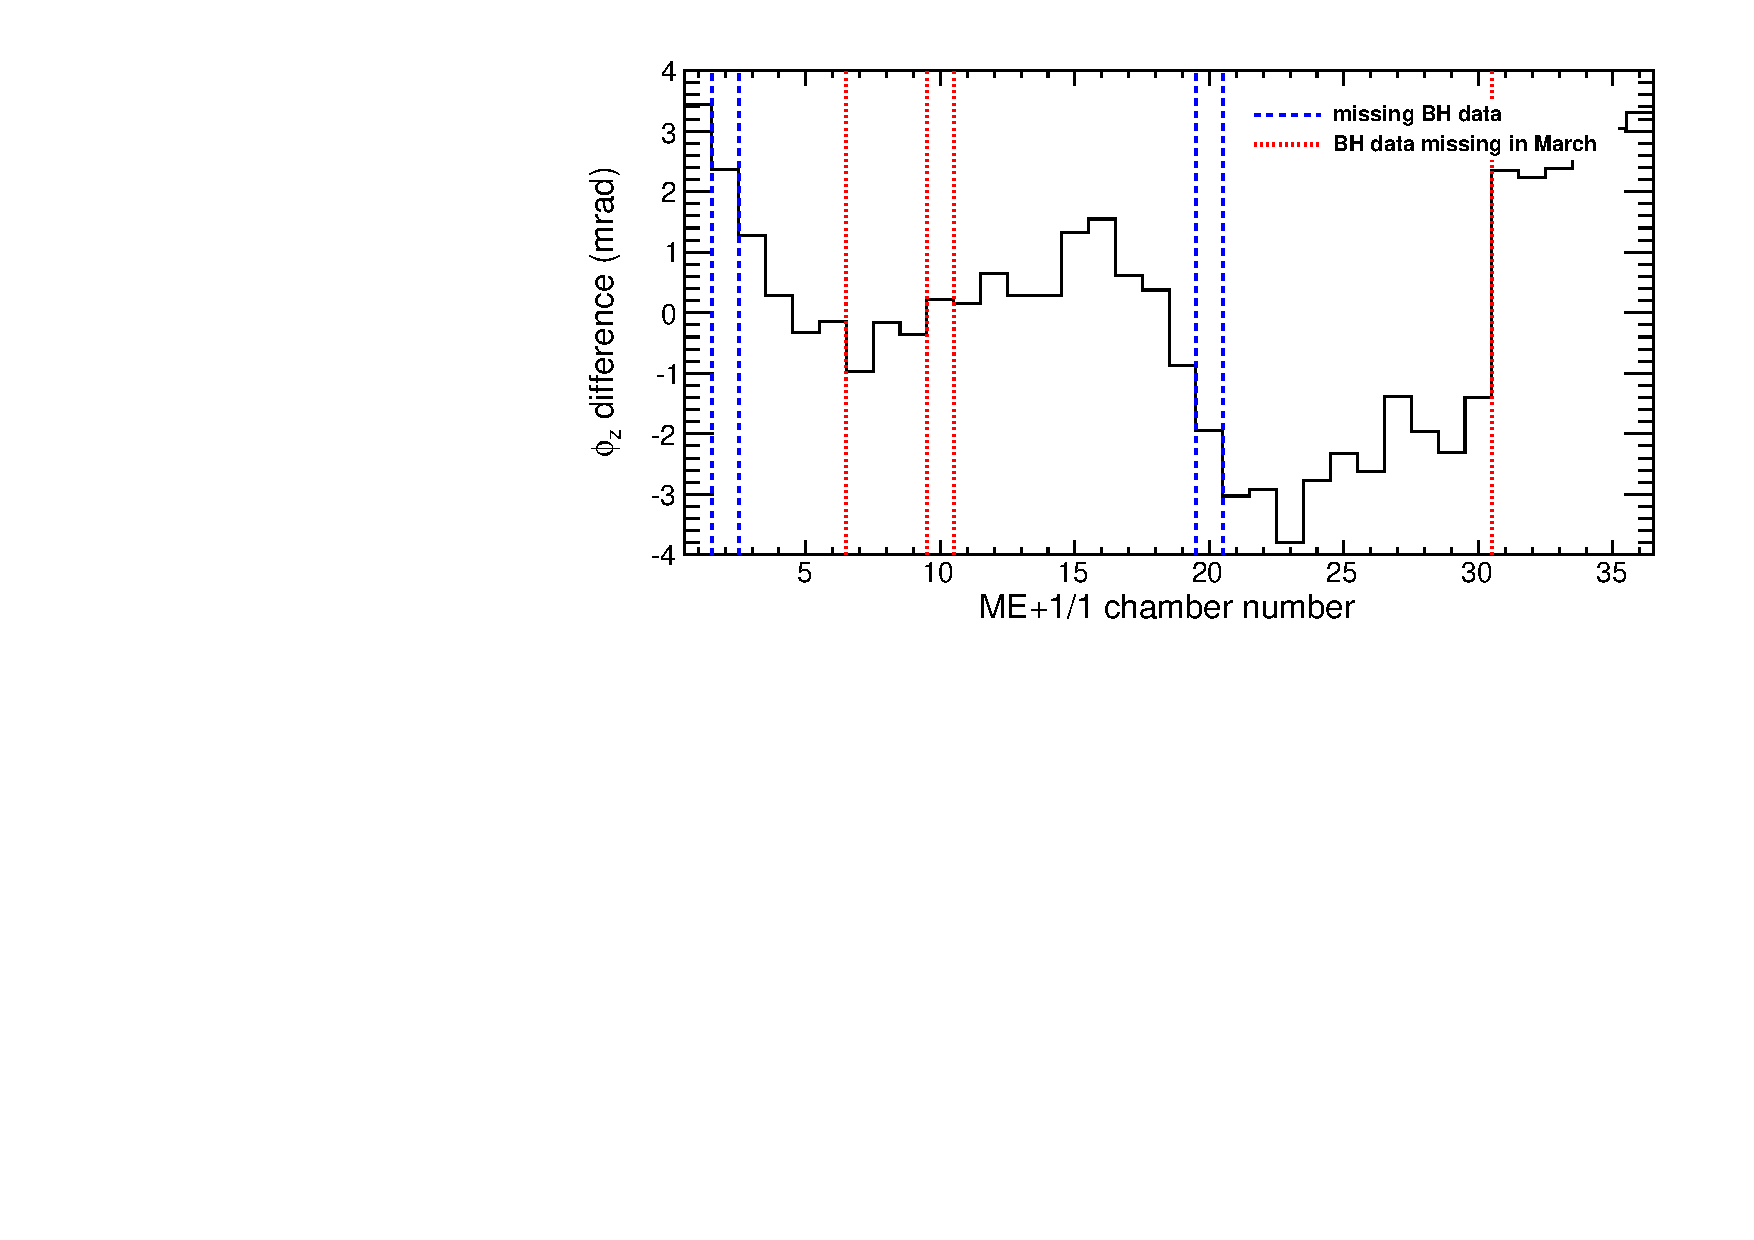
\includegraphics[width=0.45\linewidth]{TCTtoCollisions_phiz_mep11.pdf}
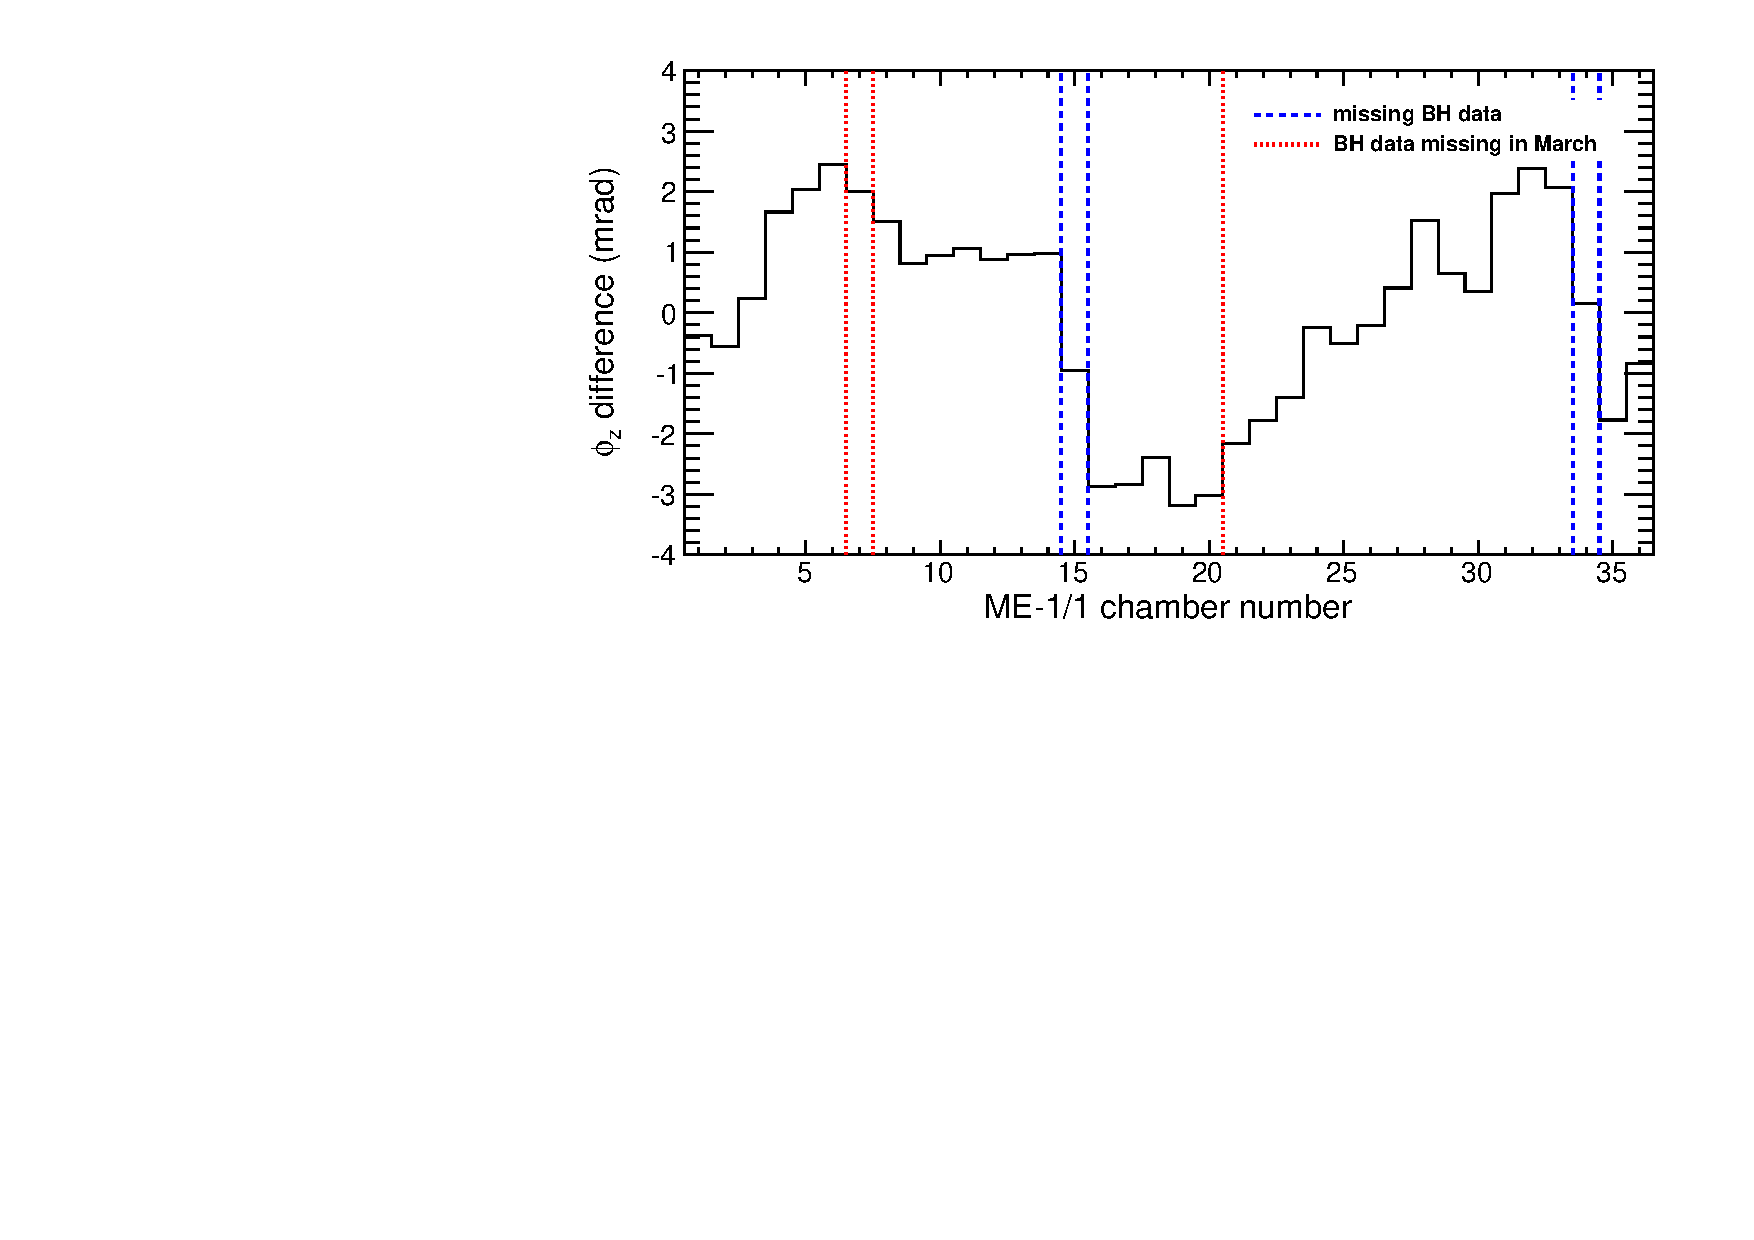
\includegraphics[width=0.45\linewidth]{TCTtoCollisions_phiz_mem11.pdf}
\end{center}

\caption{Differences in $\phi_z$ parameters between the Mar.~2010 TCT
  alignment and the summer~2010 during-collisions alignment.  The
  largest differences are in ME$\pm$1/1, usually near the missing
  overlaps measurements.  Changes in all other rings are completely
  negligible. \label{fig:TCTtoCollisions_phiz_histograms}}
\end{figure}

\subsection{Comparison of results based on old and new hardware pre-alignment}

In the second study, we aligned the same data (summer~2010) using two
pre-alignments: one with the old hardware $z$/$\phi_x$ description and
the other with the new description.  As can be seen in
Fig.~\ref{fig:oldHWtonewHW_histograms}, there are no differences in
ME1/1 (since there were no $z$/$\phi_x$ differences in ME1/1) and only
minor effects in the other rings, ranging from 0.3--0.5~mm (RMS).
Figure~\ref{fig:oldHWtonewHW_phiz_histograms} shows the same for
$\phi_z$, where all differences are completely negligible.

\begin{figure}
\begin{center}
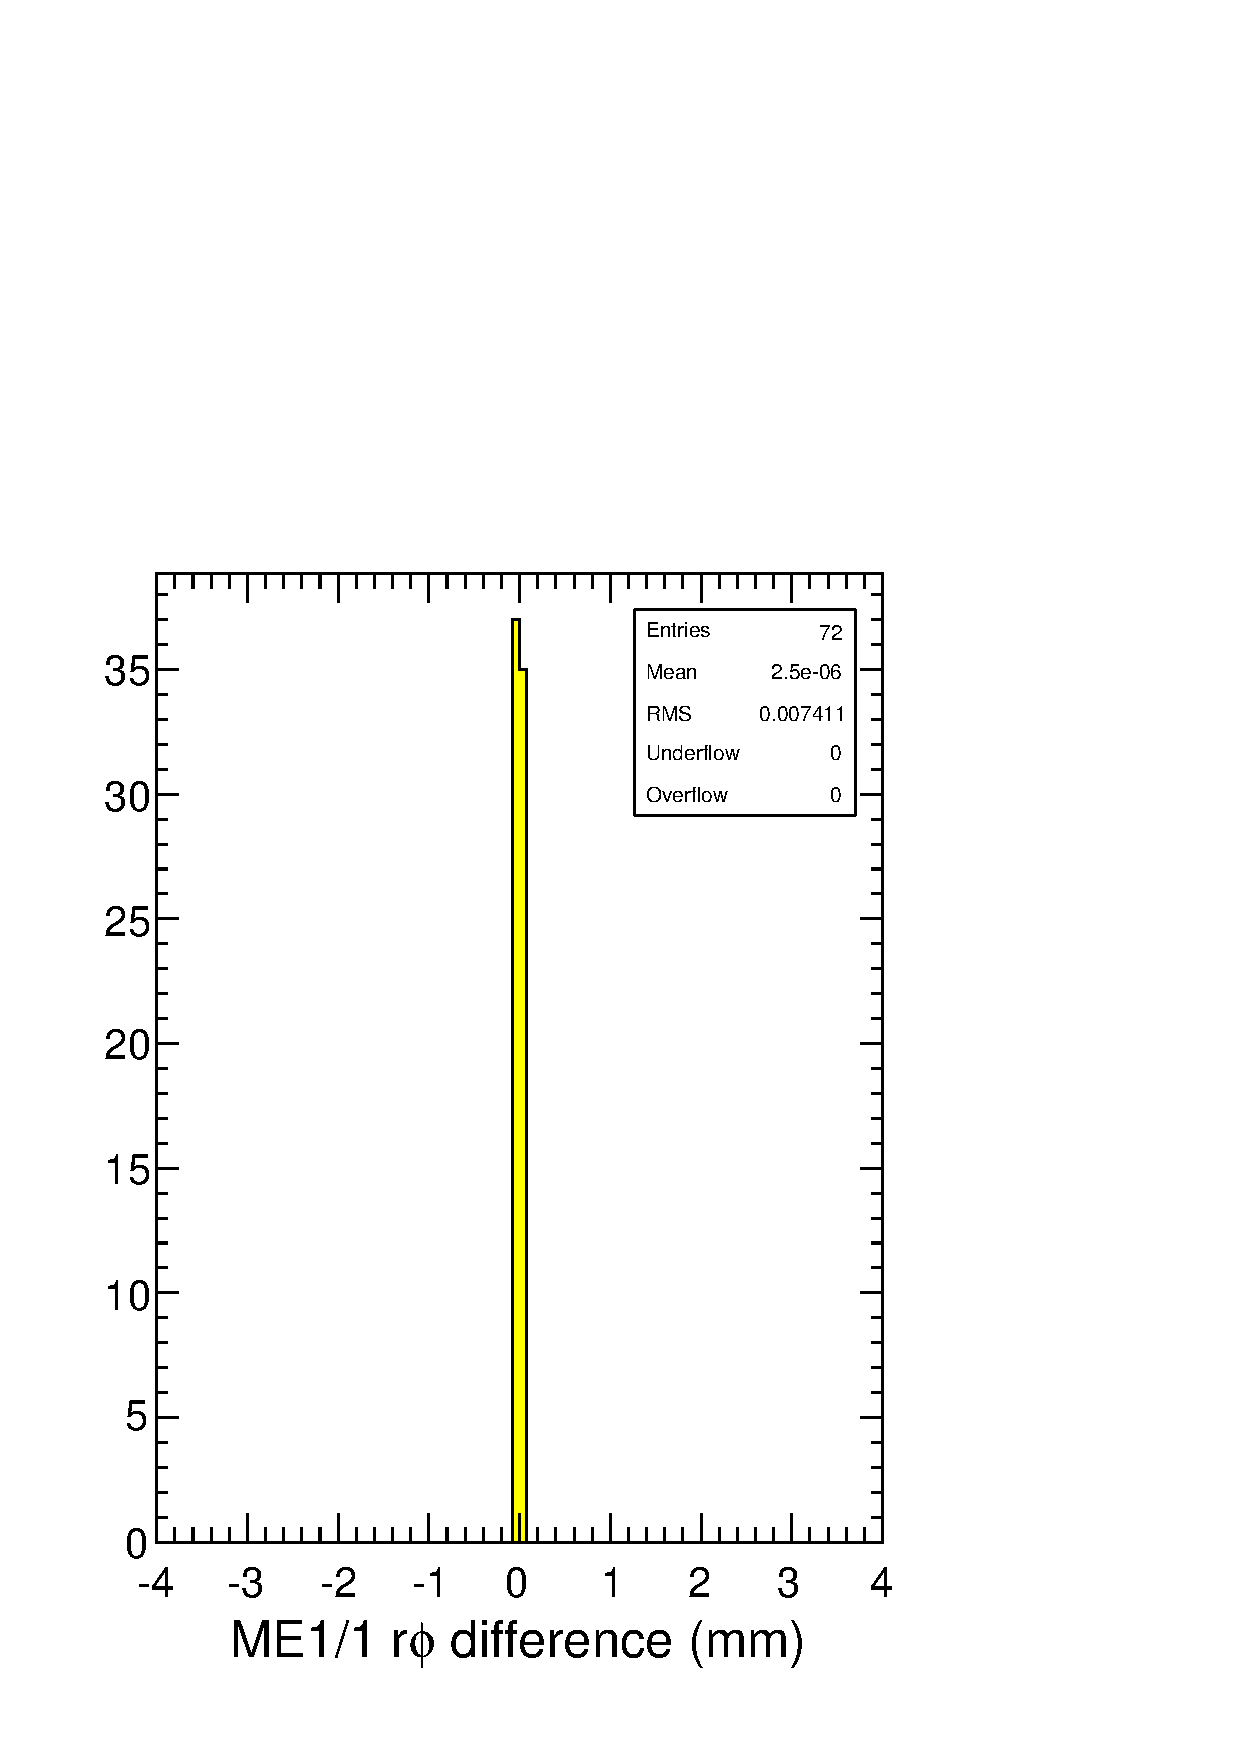
\includegraphics[width=0.32\linewidth]{oldHWtonewHW_me11.pdf}
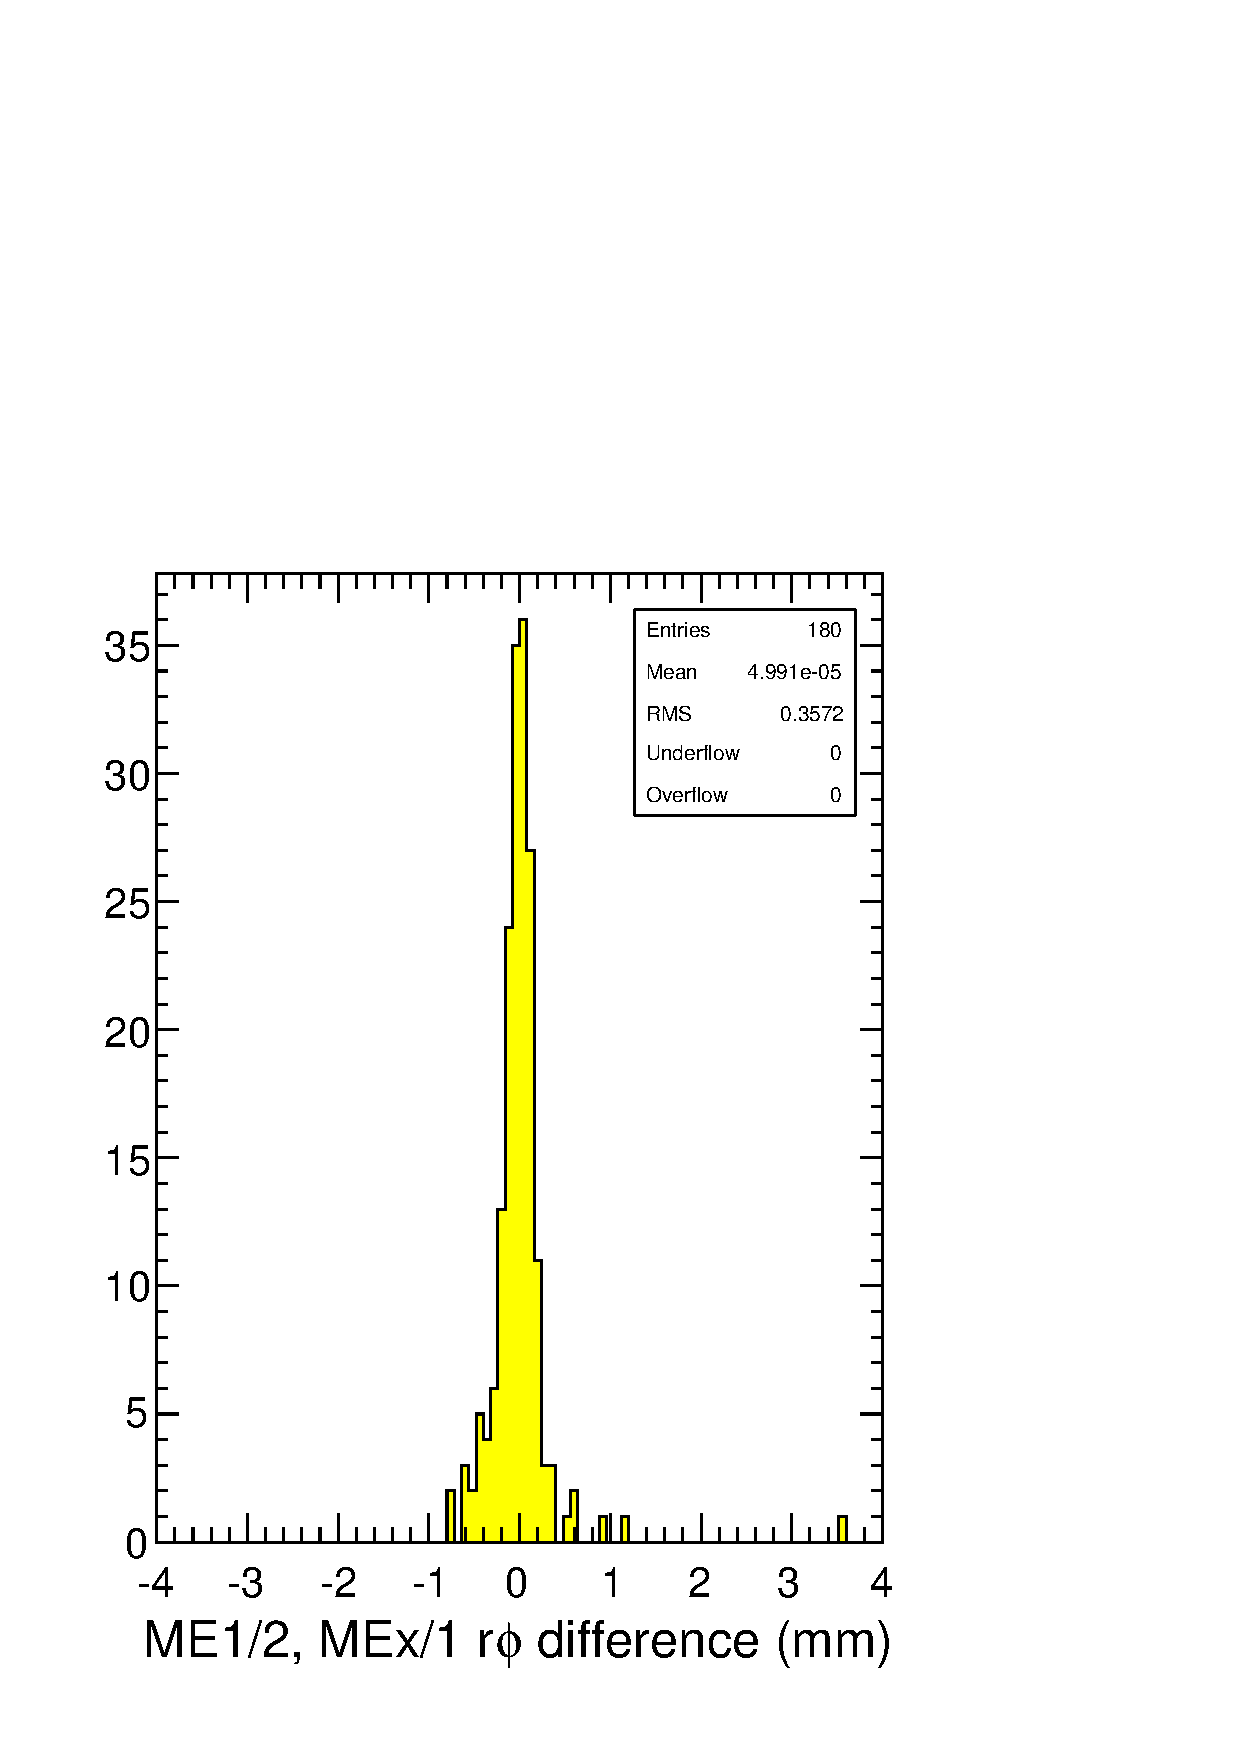
\includegraphics[width=0.32\linewidth]{oldHWtonewHW_inner.pdf}
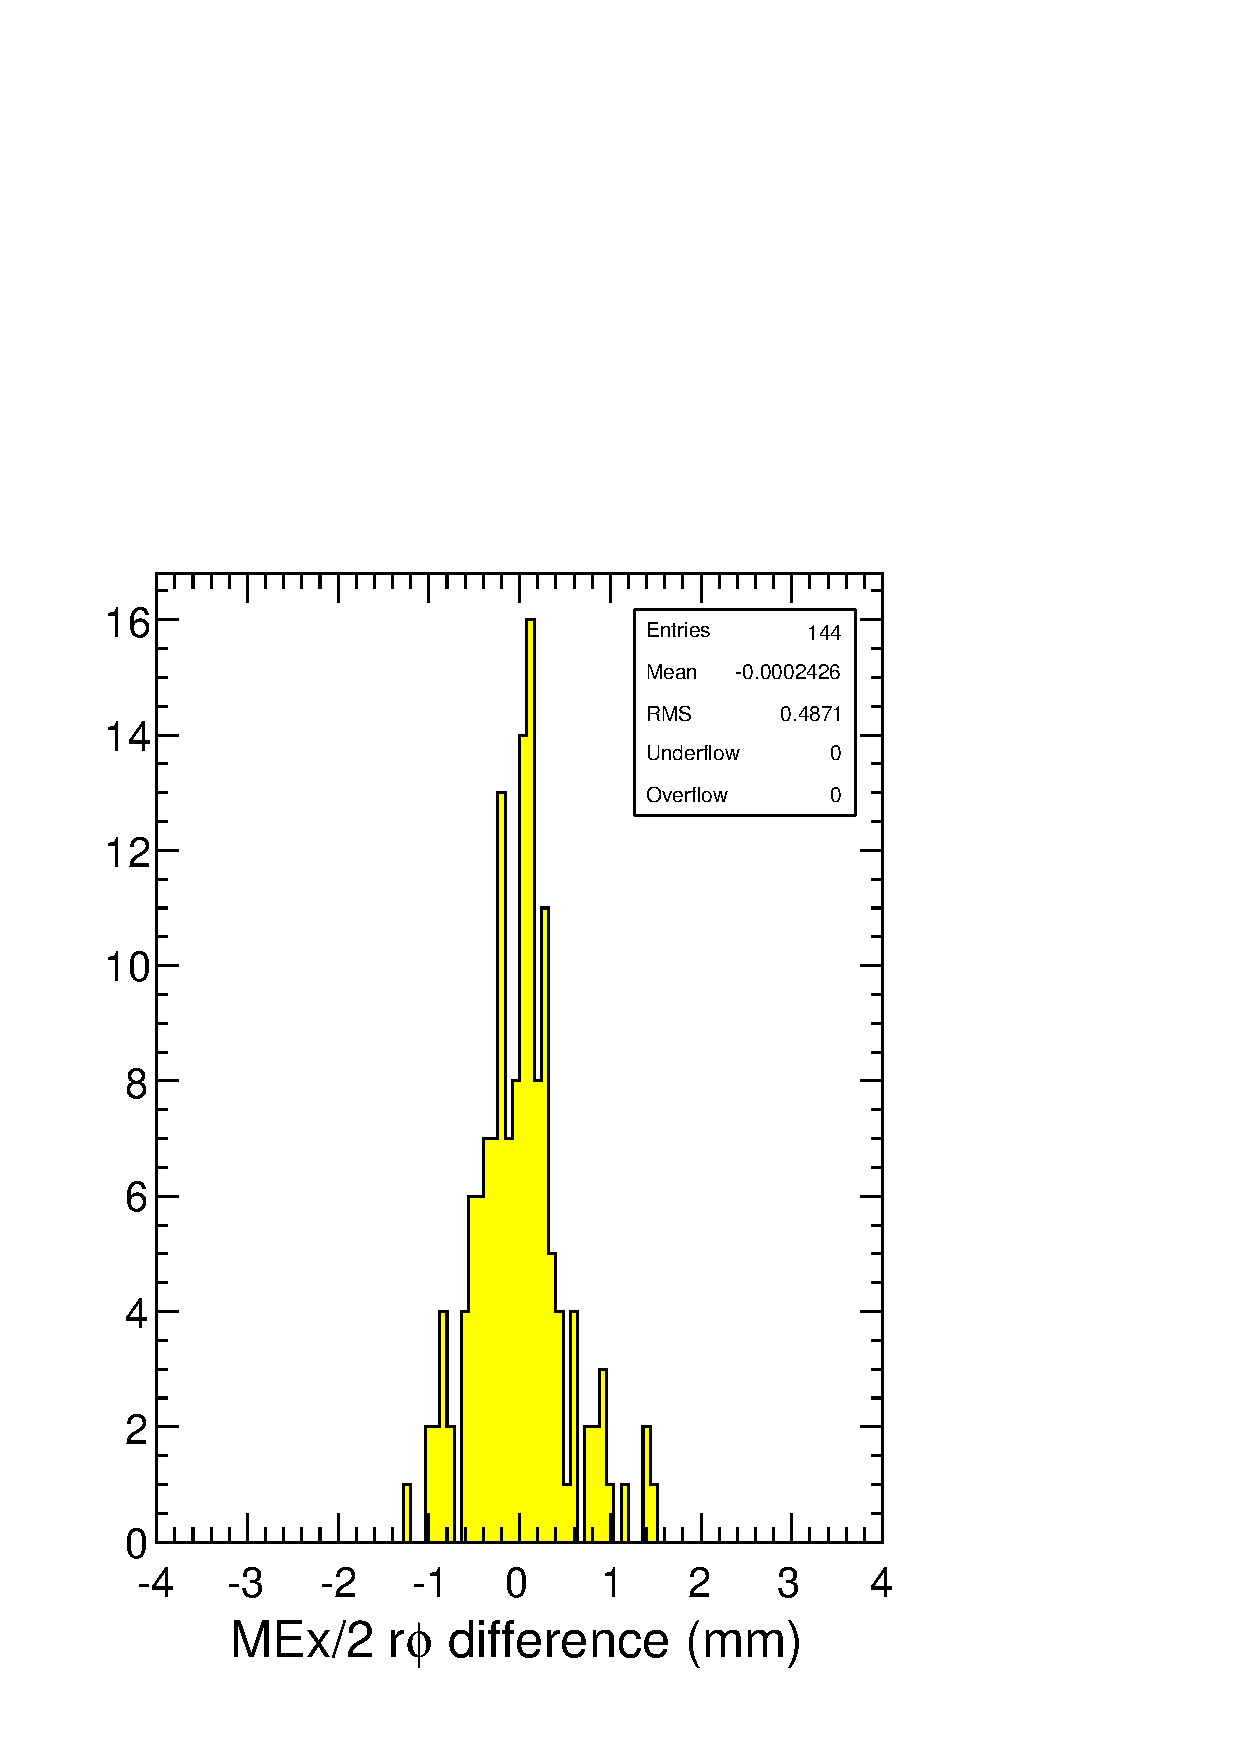
\includegraphics[width=0.32\linewidth]{oldHWtonewHW_outer.pdf}
\end{center}

\caption{Differences in $r\phi$ parameters between a summer~2010
  alignment with old HW $z$/$\phi_x$ description and the new HW
  $z$/$\phi_x$ update.  No changes in these parameters were made in
  ME1/1, so ME1/1 are exactly the same.  Other rings are sensitive at
  the level of 0.3--0.5~mm (RMS). \label{fig:oldHWtonewHW_histograms}}
\end{figure}

\begin{figure}
\begin{center}
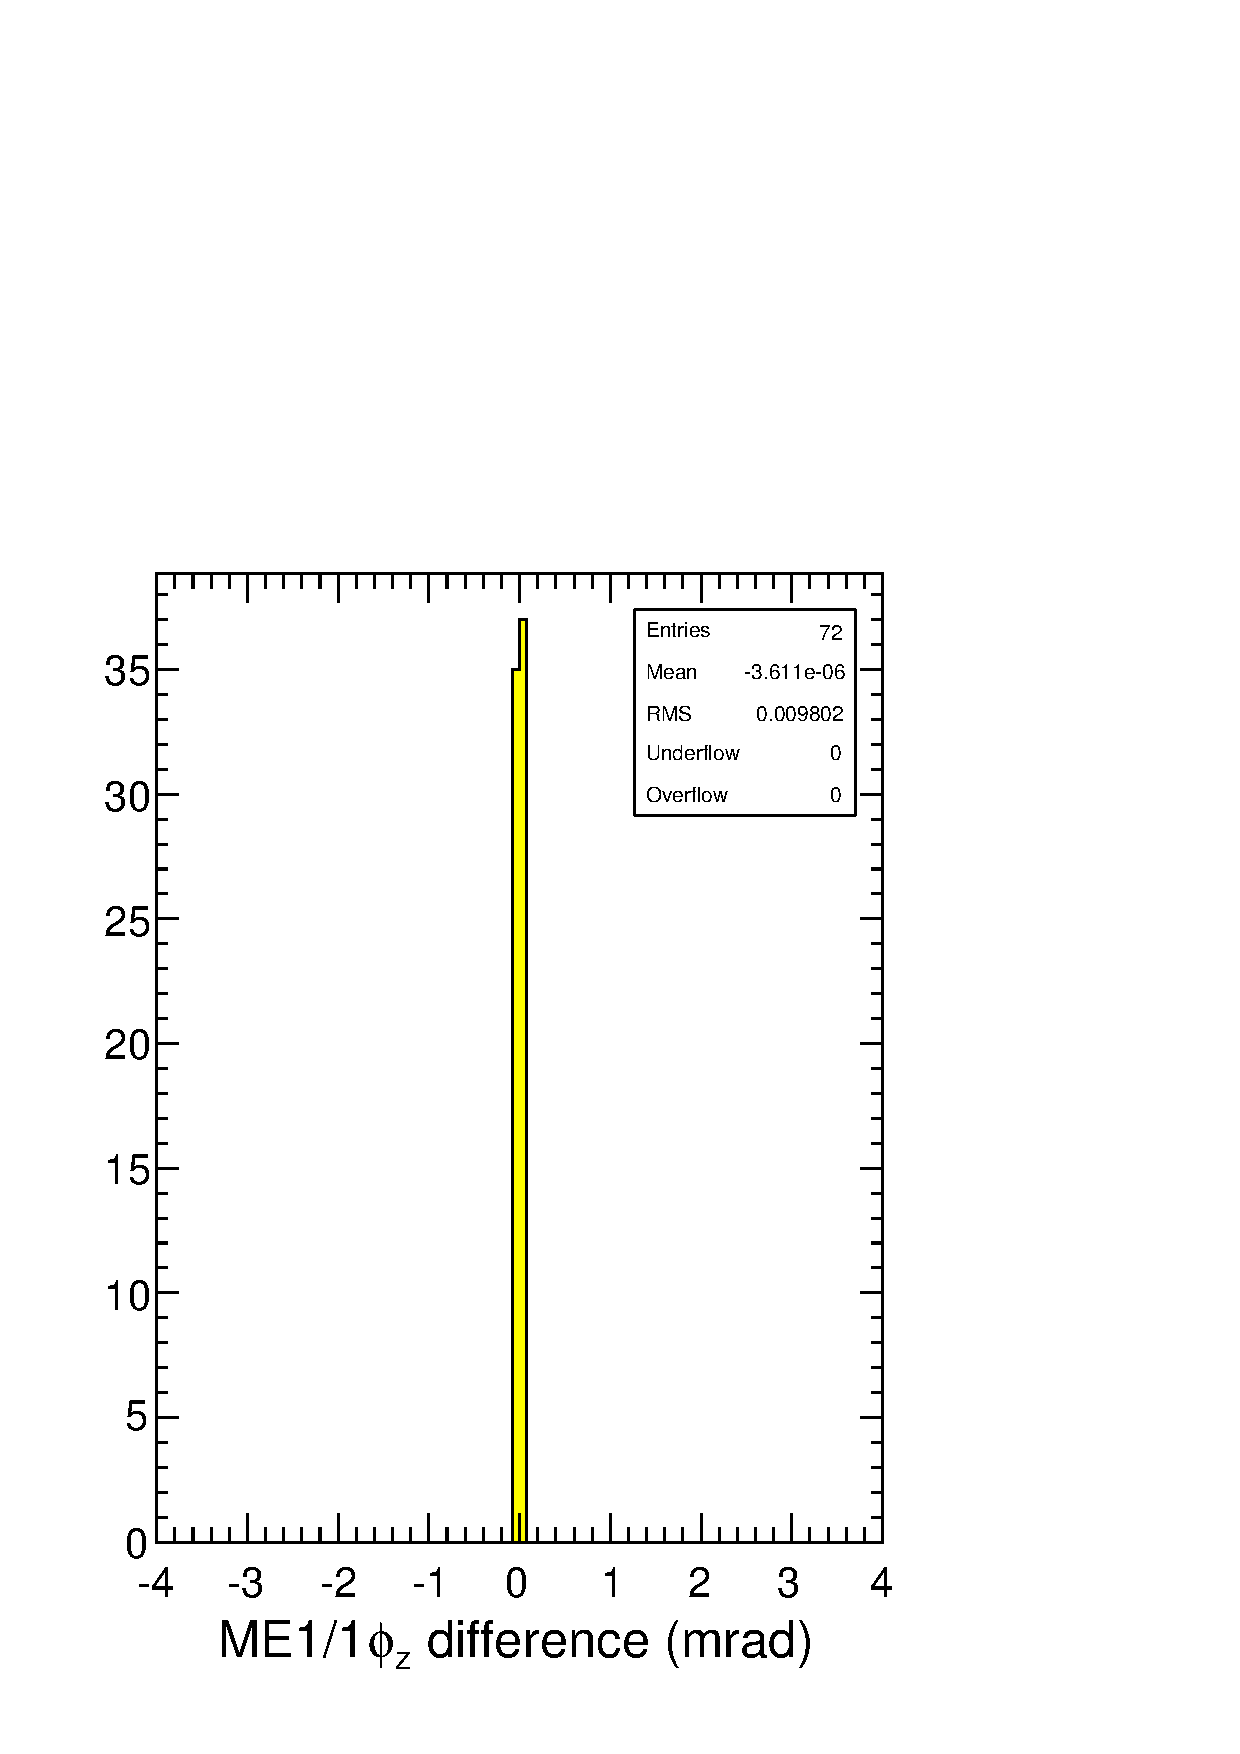
\includegraphics[width=0.32\linewidth]{oldHWtonewHW_phiz_me11.pdf}
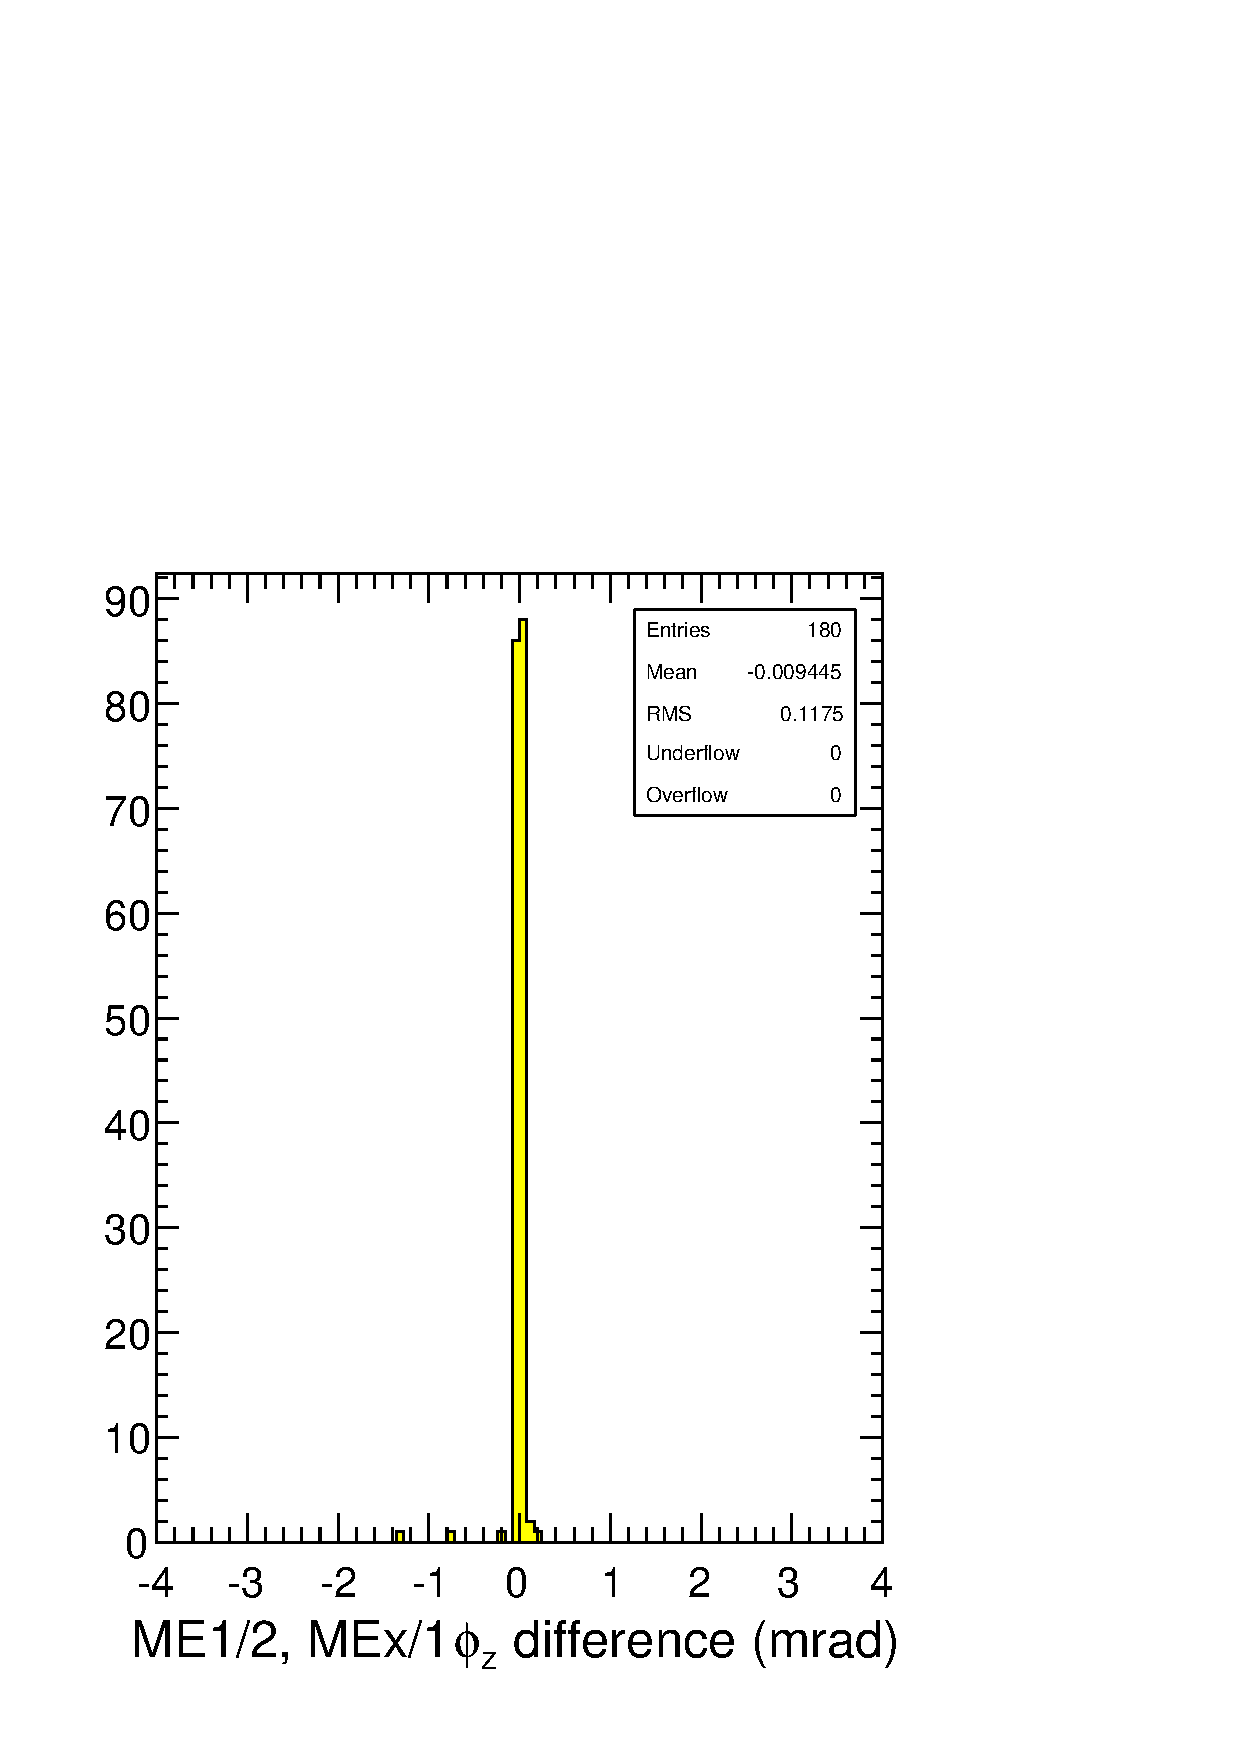
\includegraphics[width=0.32\linewidth]{oldHWtonewHW_phiz_inner.pdf}
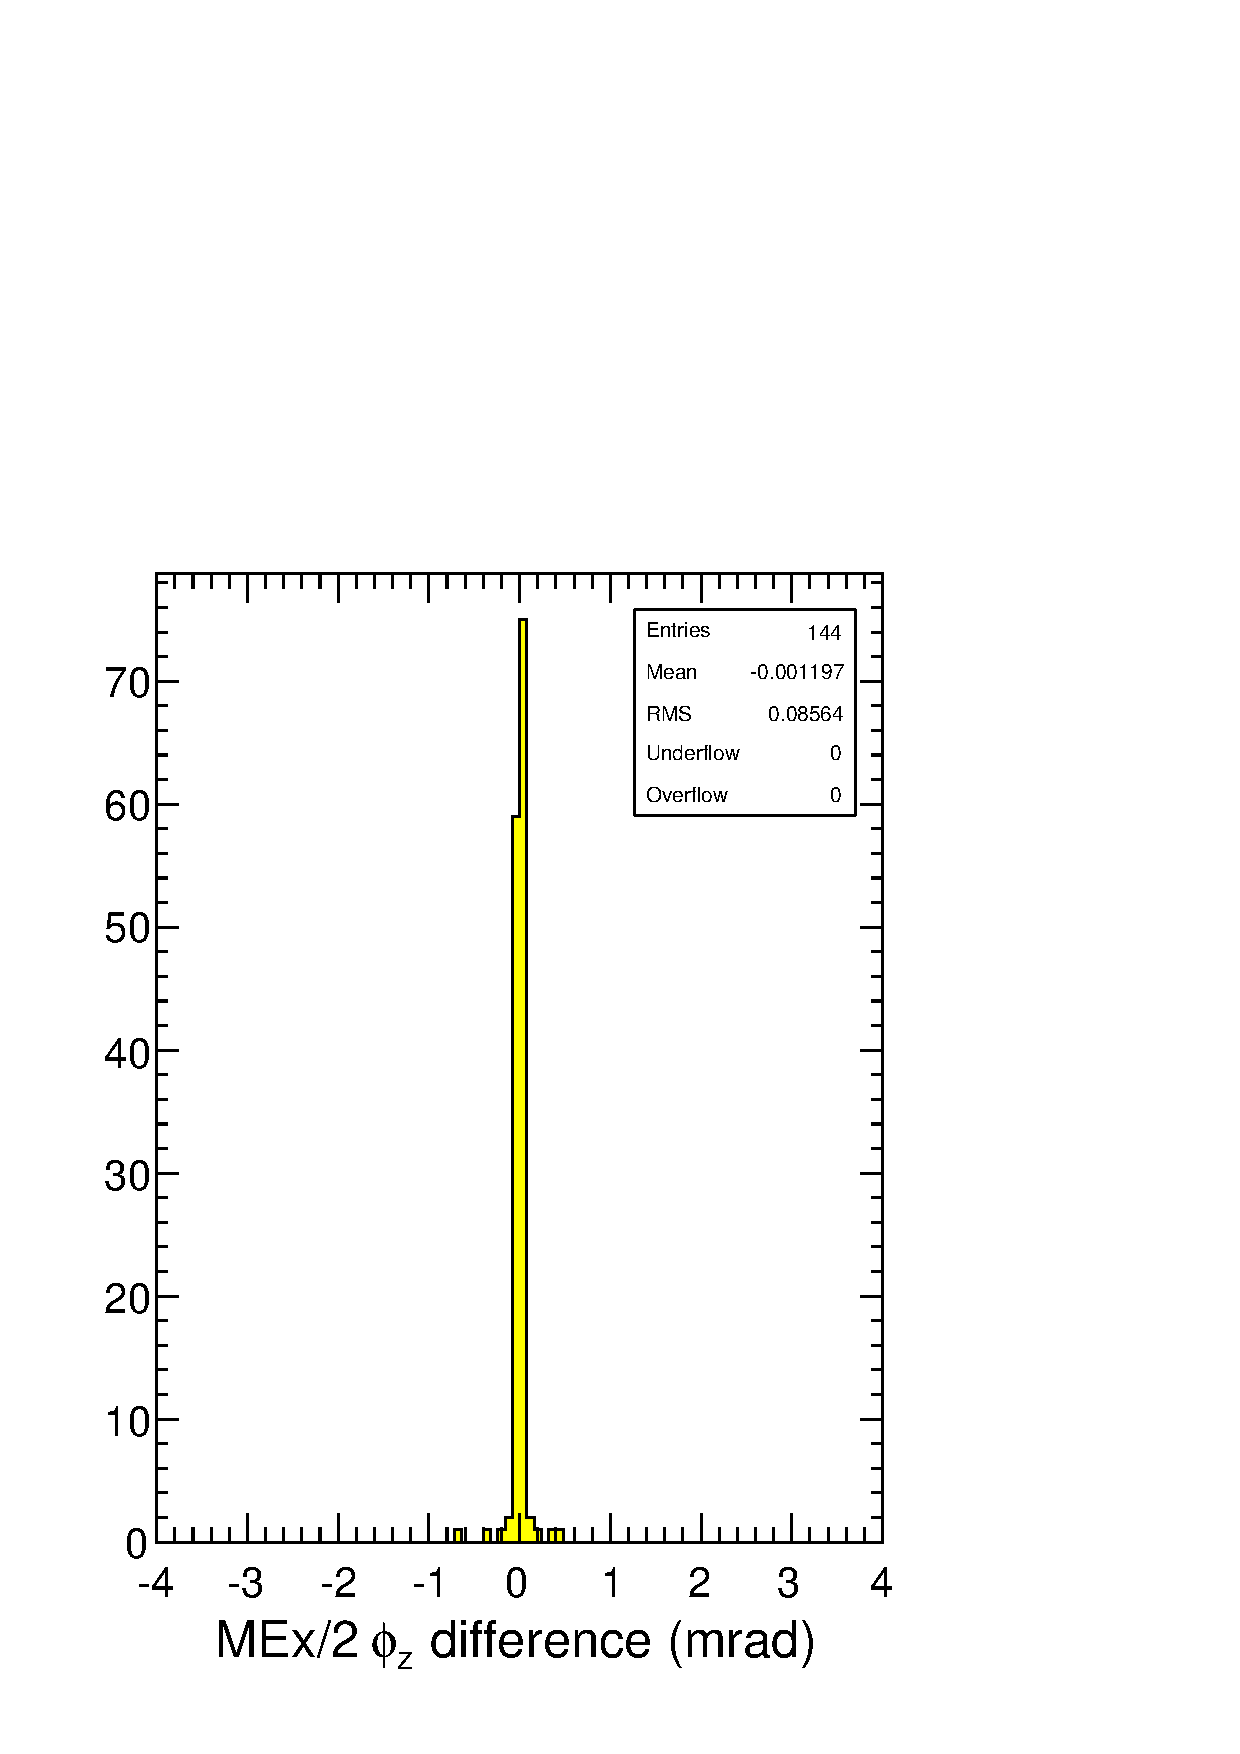
\includegraphics[width=0.32\linewidth]{oldHWtonewHW_phiz_outer.pdf}
\end{center}

\caption{Differences in $\phi_z$ parameters between a summer~2010
  alignment with old HW $z$/$\phi_x$ description and the new HW
  $z$/$\phi_x$ update.  All $\phi_z$ differences are completely
  negligible. \label{fig:oldHWtonewHW_phiz_histograms}}
\end{figure}

\subsection{Comparison of results with and without $\phi_y$ pre-alignment}

The next test compared two geometries aligned with the same data
(summer~2010) using two pre-alignments: one with $\phi_y$ corrections
derived from data, and the other without.  One might imagine $\phi_y$
differences to have an effect on $r\phi$, since this angle would bias
the slope of all segments in a chamber (see Fig.~\ref{fig:overlaps}).
However, the slope resolution is 8~mrad and $\phi_y$ corrections were
typically only a few mrad (see
Fig.~\ref{fig:offsetResiduals_badphiy}), so the result is not
particularly sensitive to these changes.
Figures~\ref{fig:noPhiYtoPhiY_histograms} and
\ref{fig:noPhiYtoPhiY_phiz_histograms} show the $r\phi$ and $\phi_z$
sensitivity to the $\phi_y$ pre-alignment: about 0.25--0.5~mm in
$r\phi$ and negligible in $\phi_z$.

\begin{figure}
\begin{center}
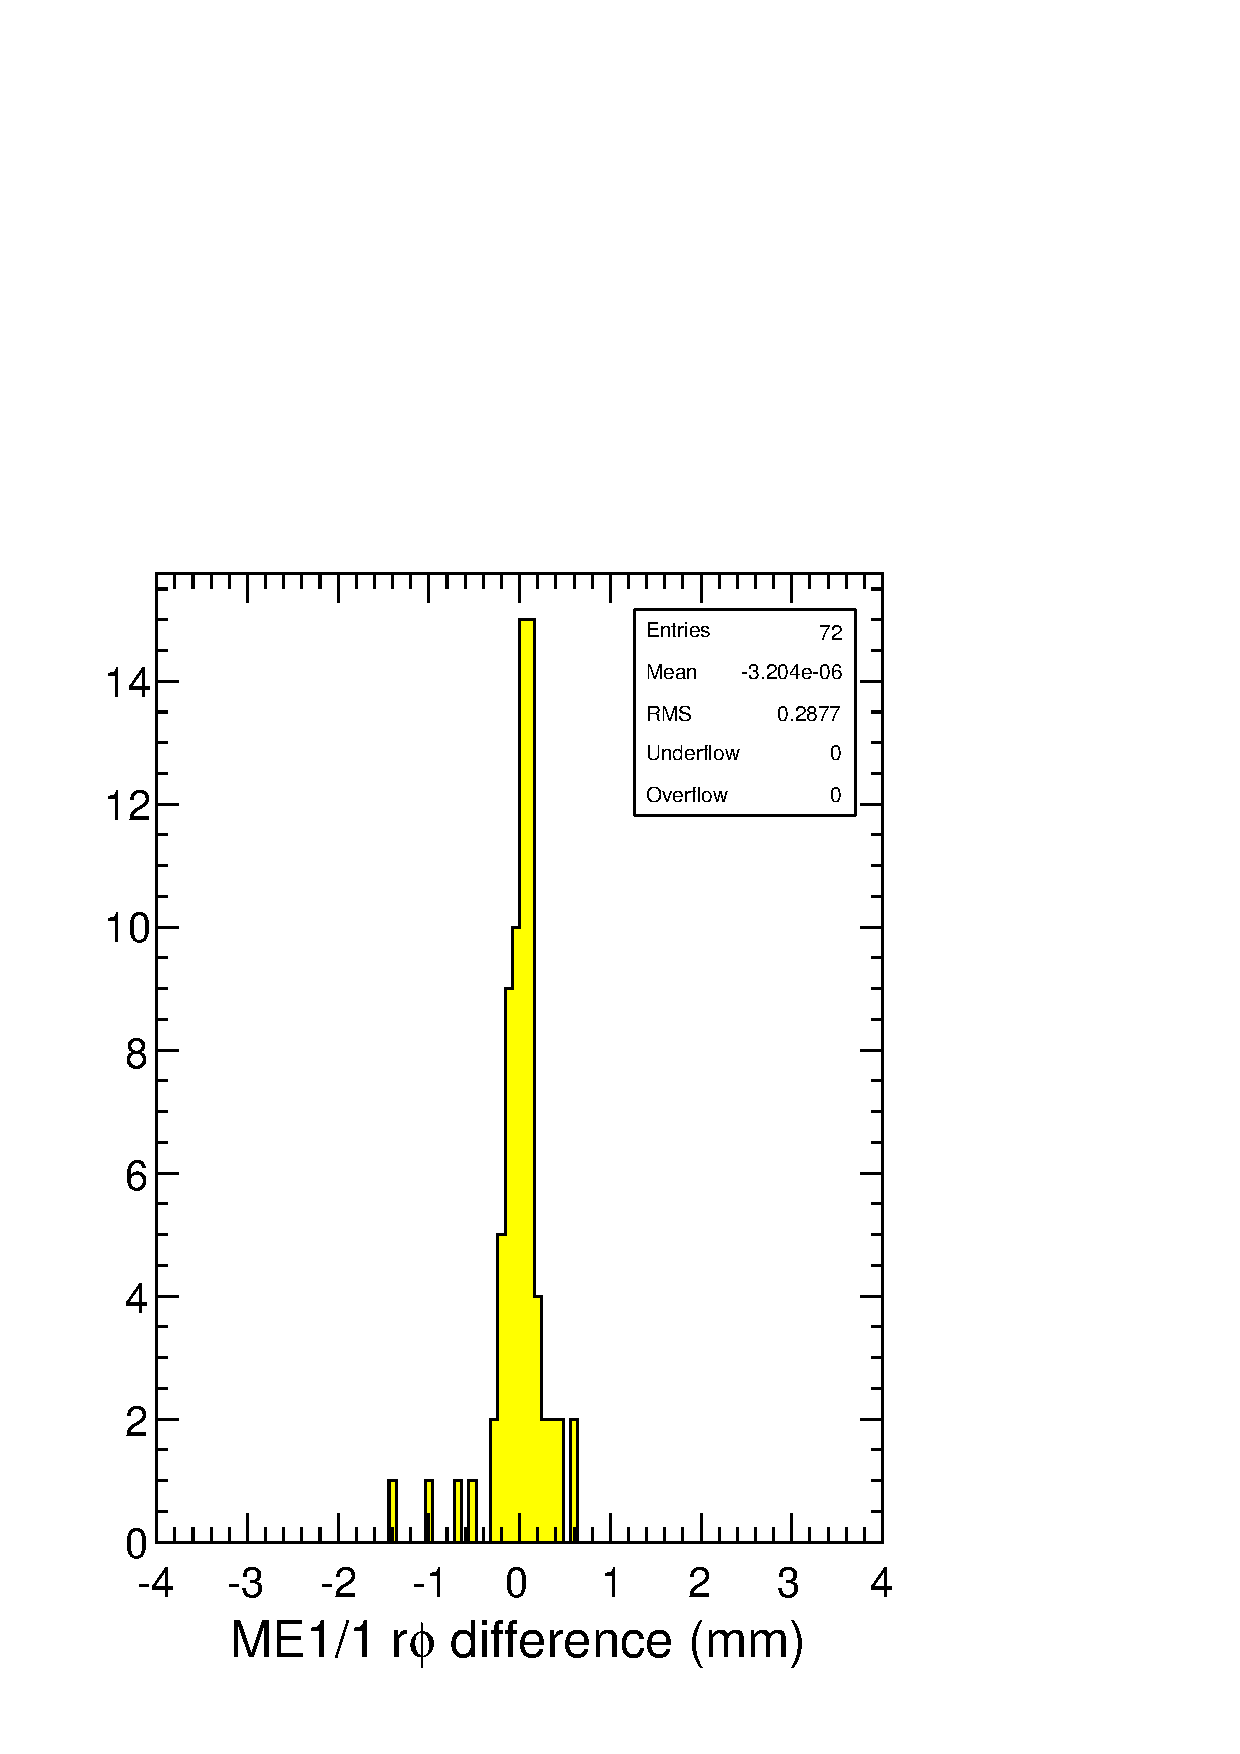
\includegraphics[width=0.32\linewidth]{noPhiYtoPhiY_me11.pdf}
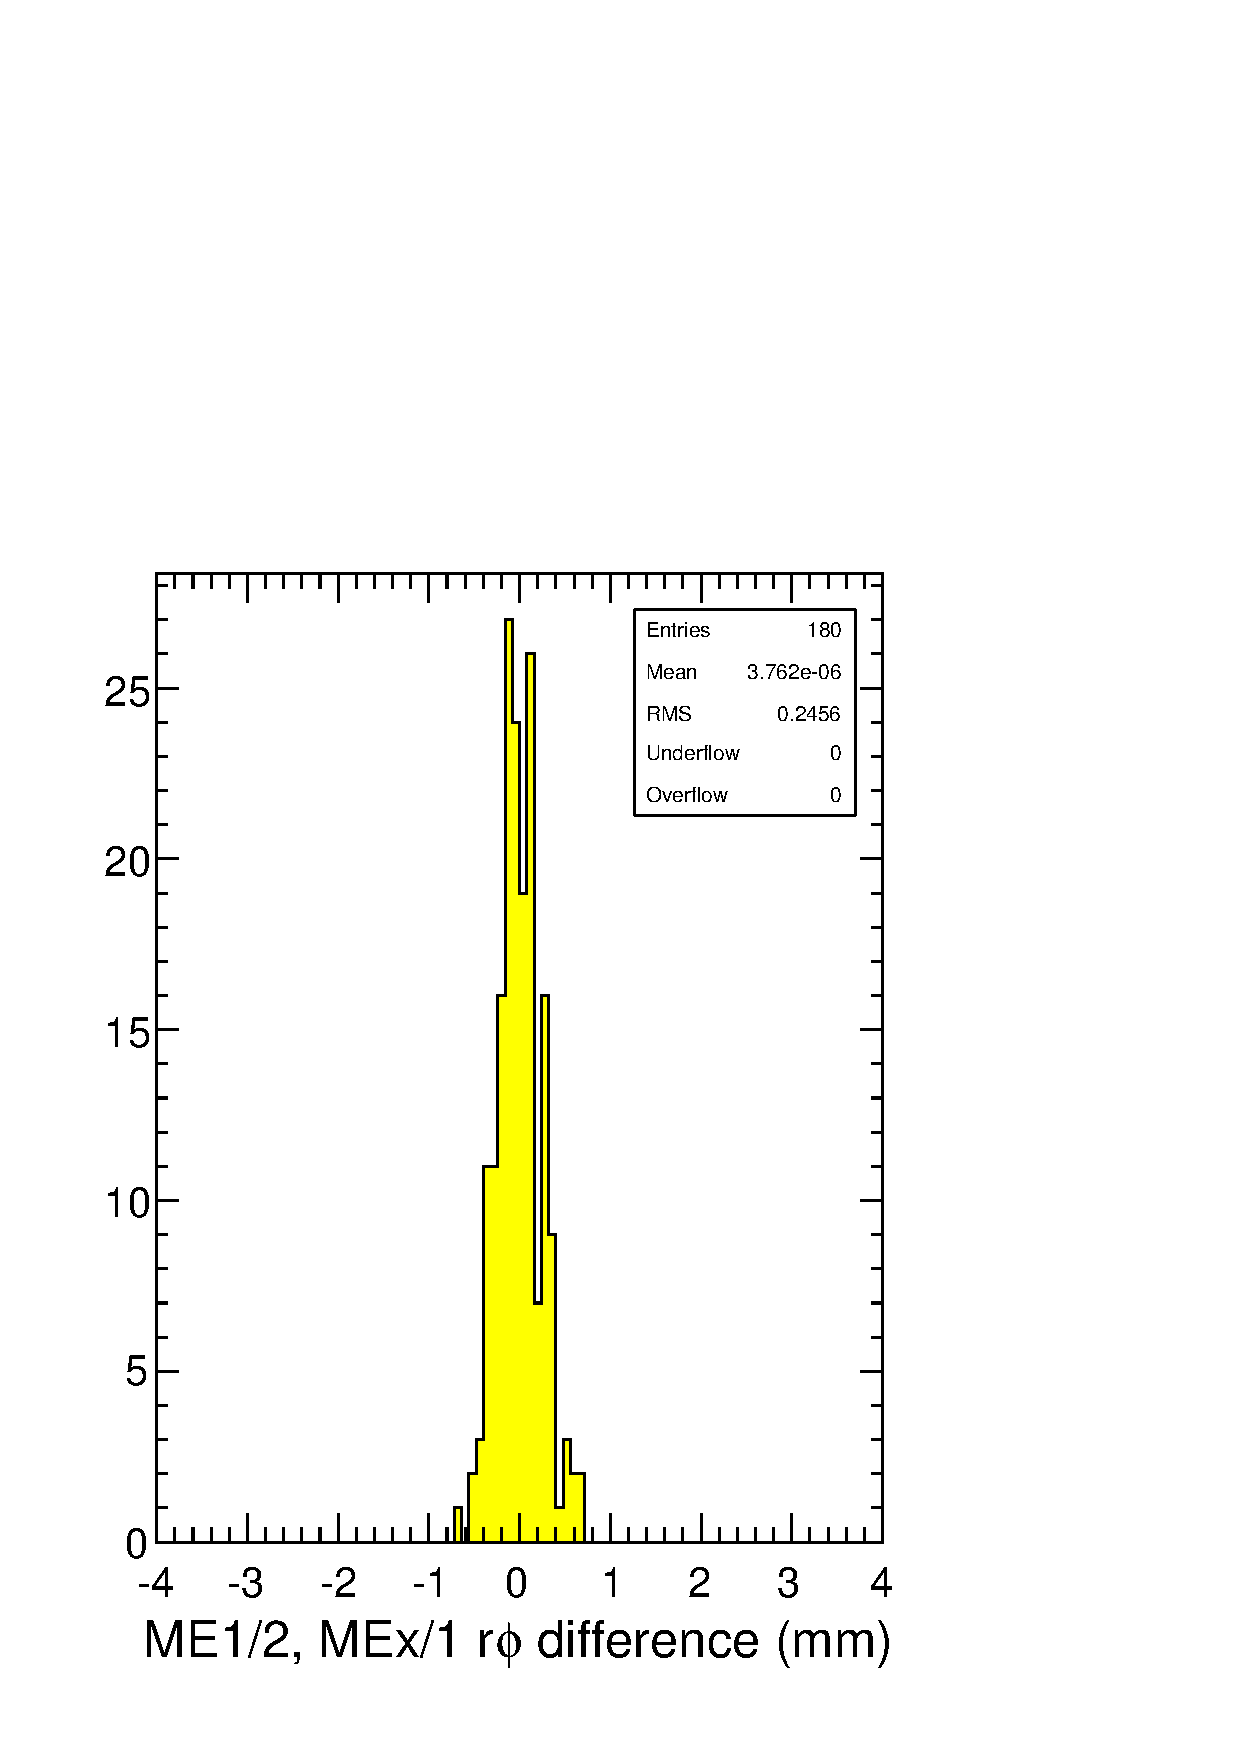
\includegraphics[width=0.32\linewidth]{noPhiYtoPhiY_inner.pdf}
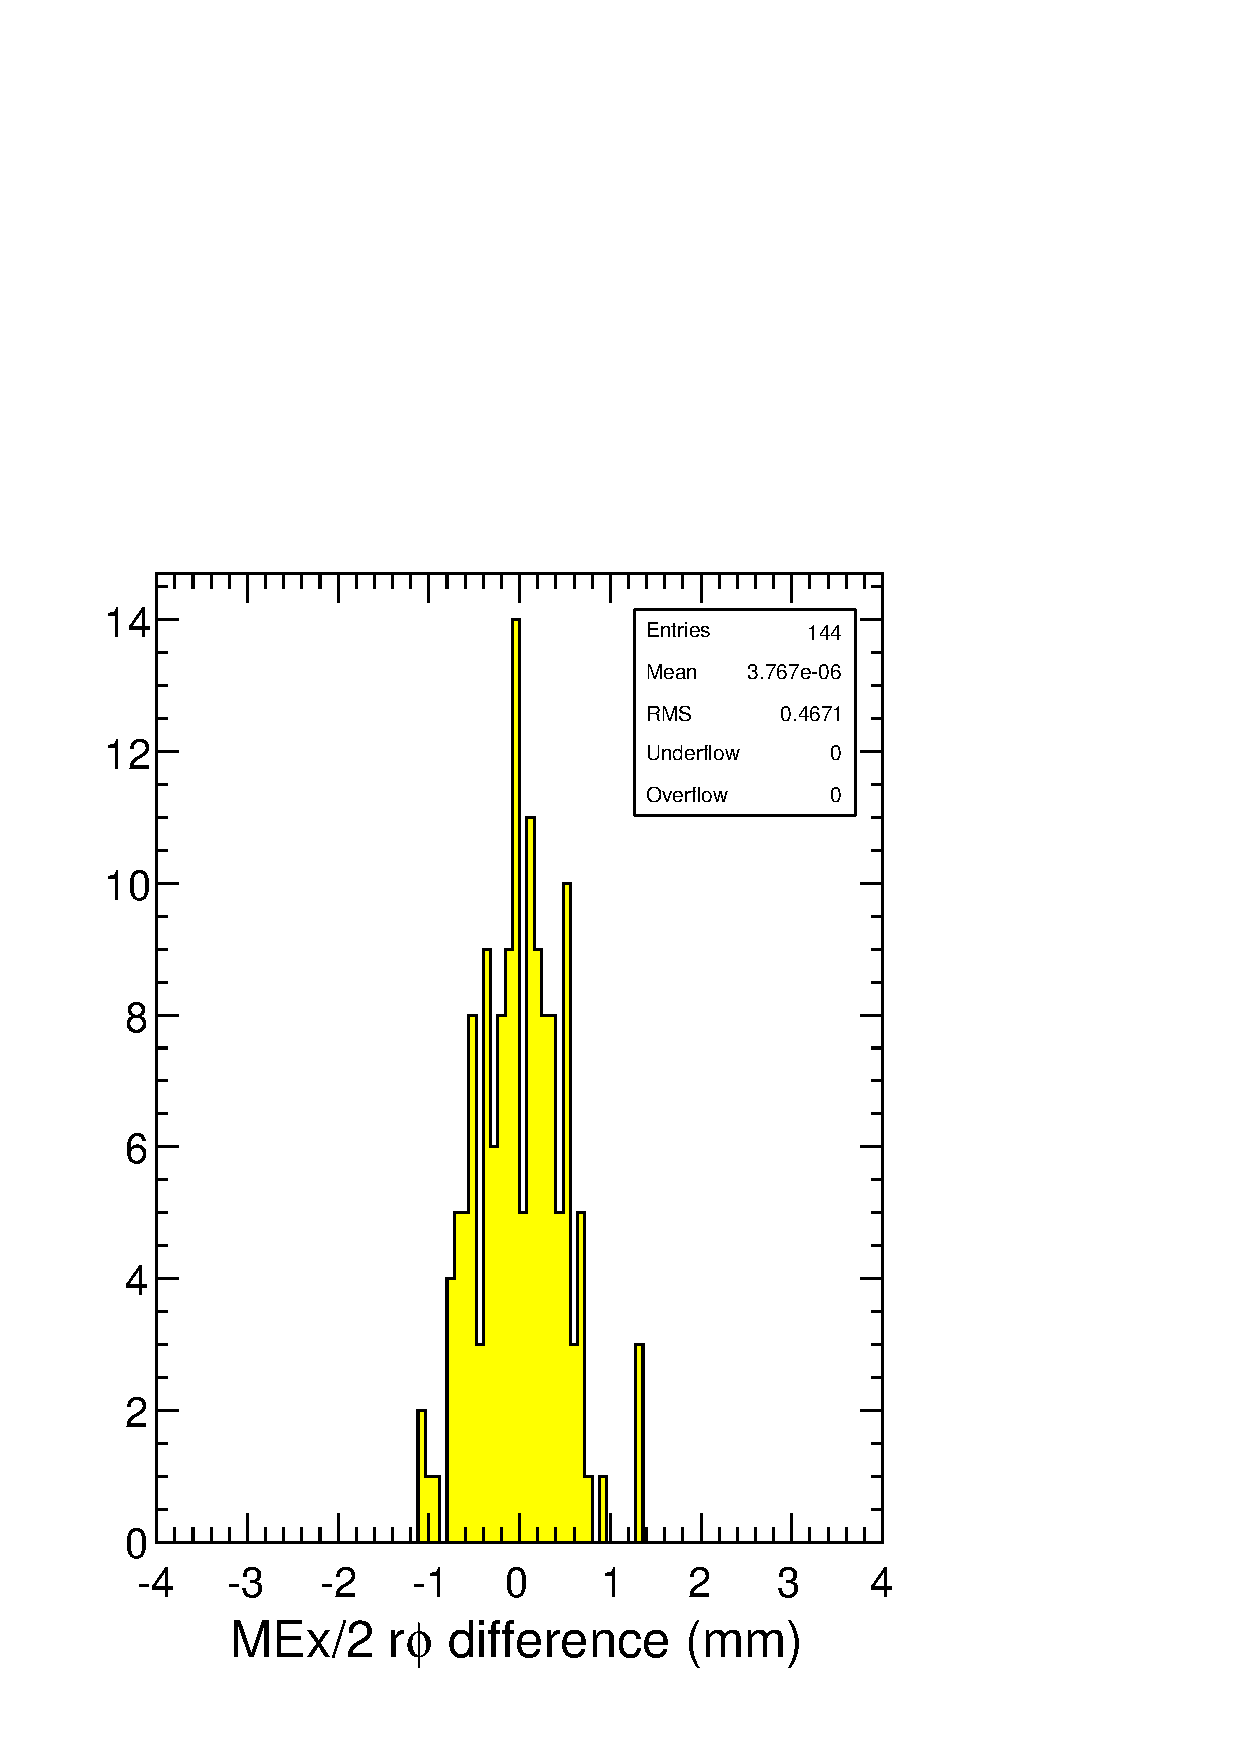
\includegraphics[width=0.32\linewidth]{noPhiYtoPhiY_outer.pdf}
\end{center}

\caption{Differences in $r\phi$ parameters between a summer~2010
  alignment with and without $\phi_y$ pre-alignment.  The $r\phi$
  differences are sensitive at the level of
  0.25--0.5~mm (RMS). \label{fig:noPhiYtoPhiY_histograms}}
\end{figure}

\begin{figure}
\begin{center}
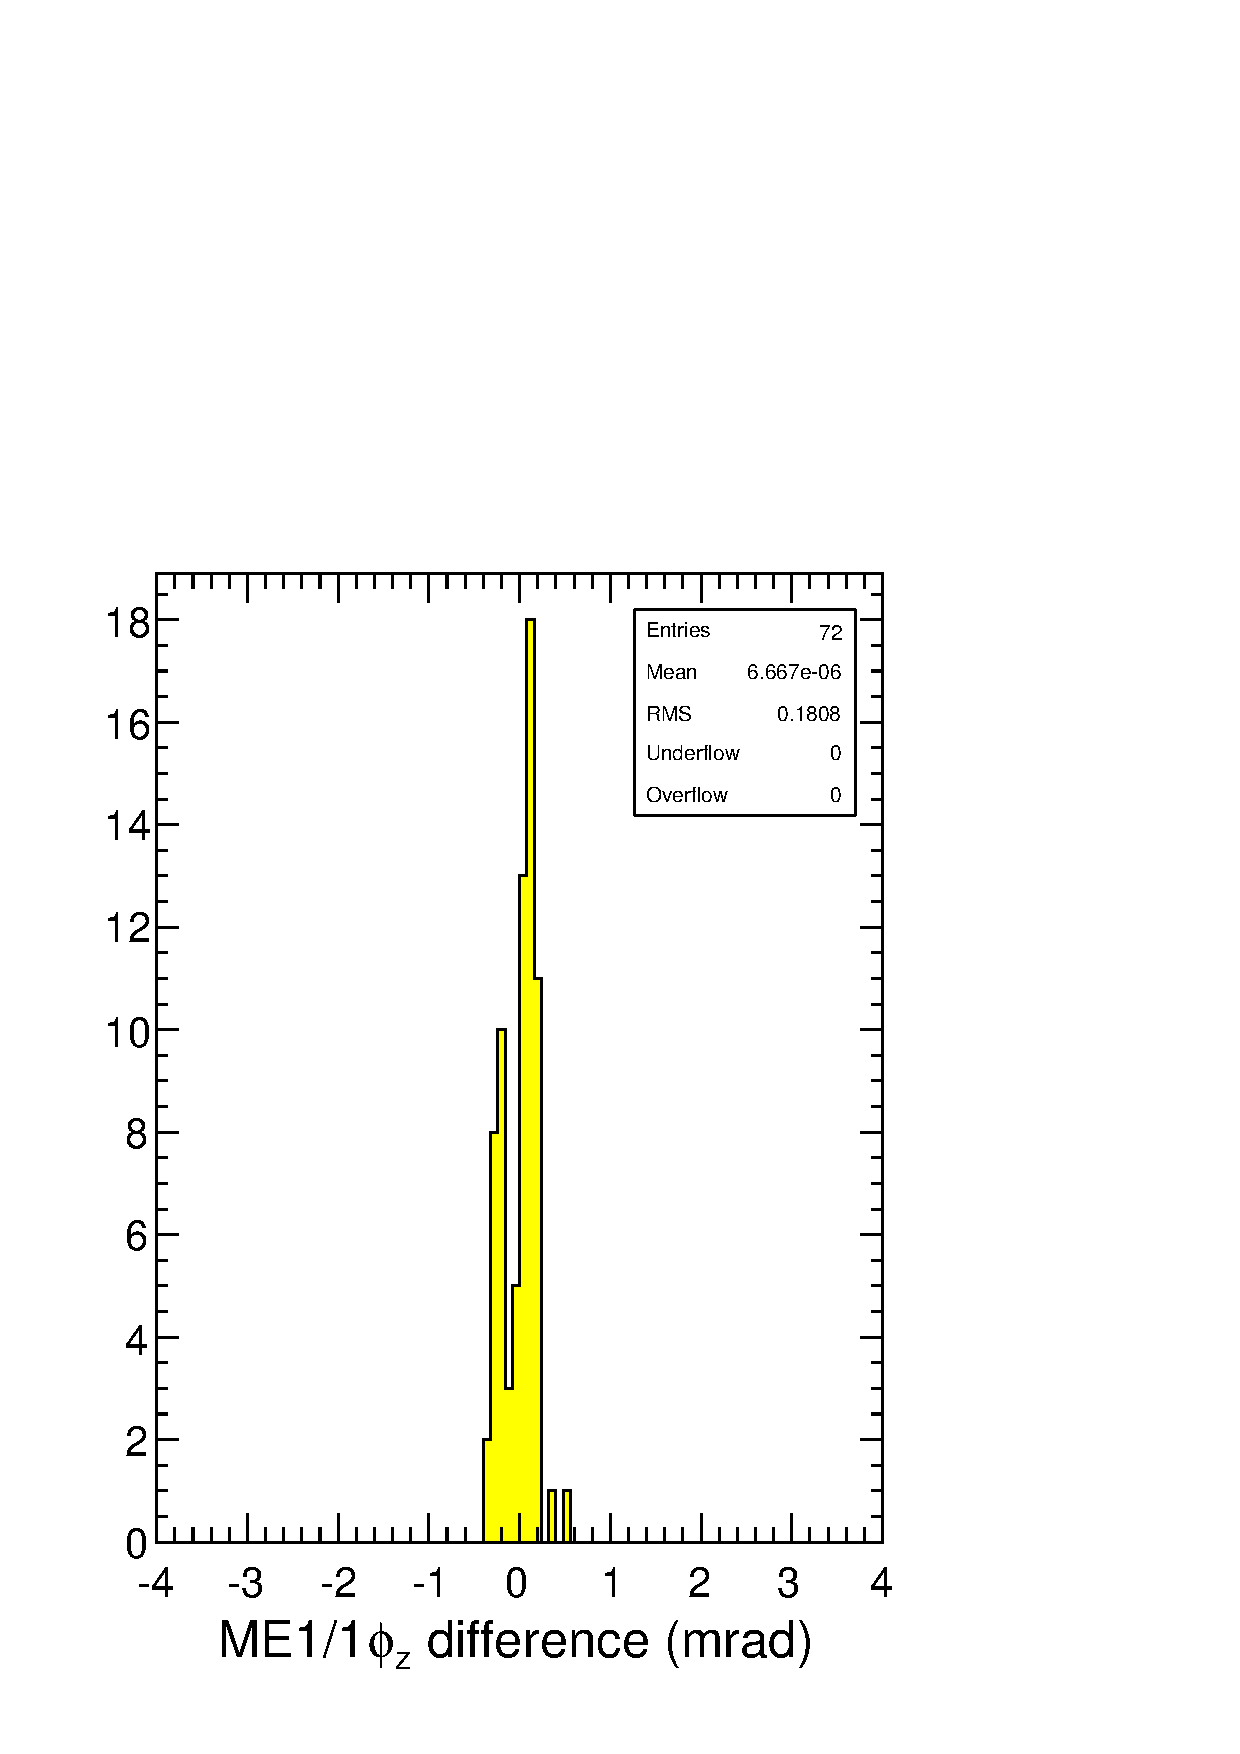
\includegraphics[width=0.32\linewidth]{noPhiYtoPhiY_phiz_me11.pdf}
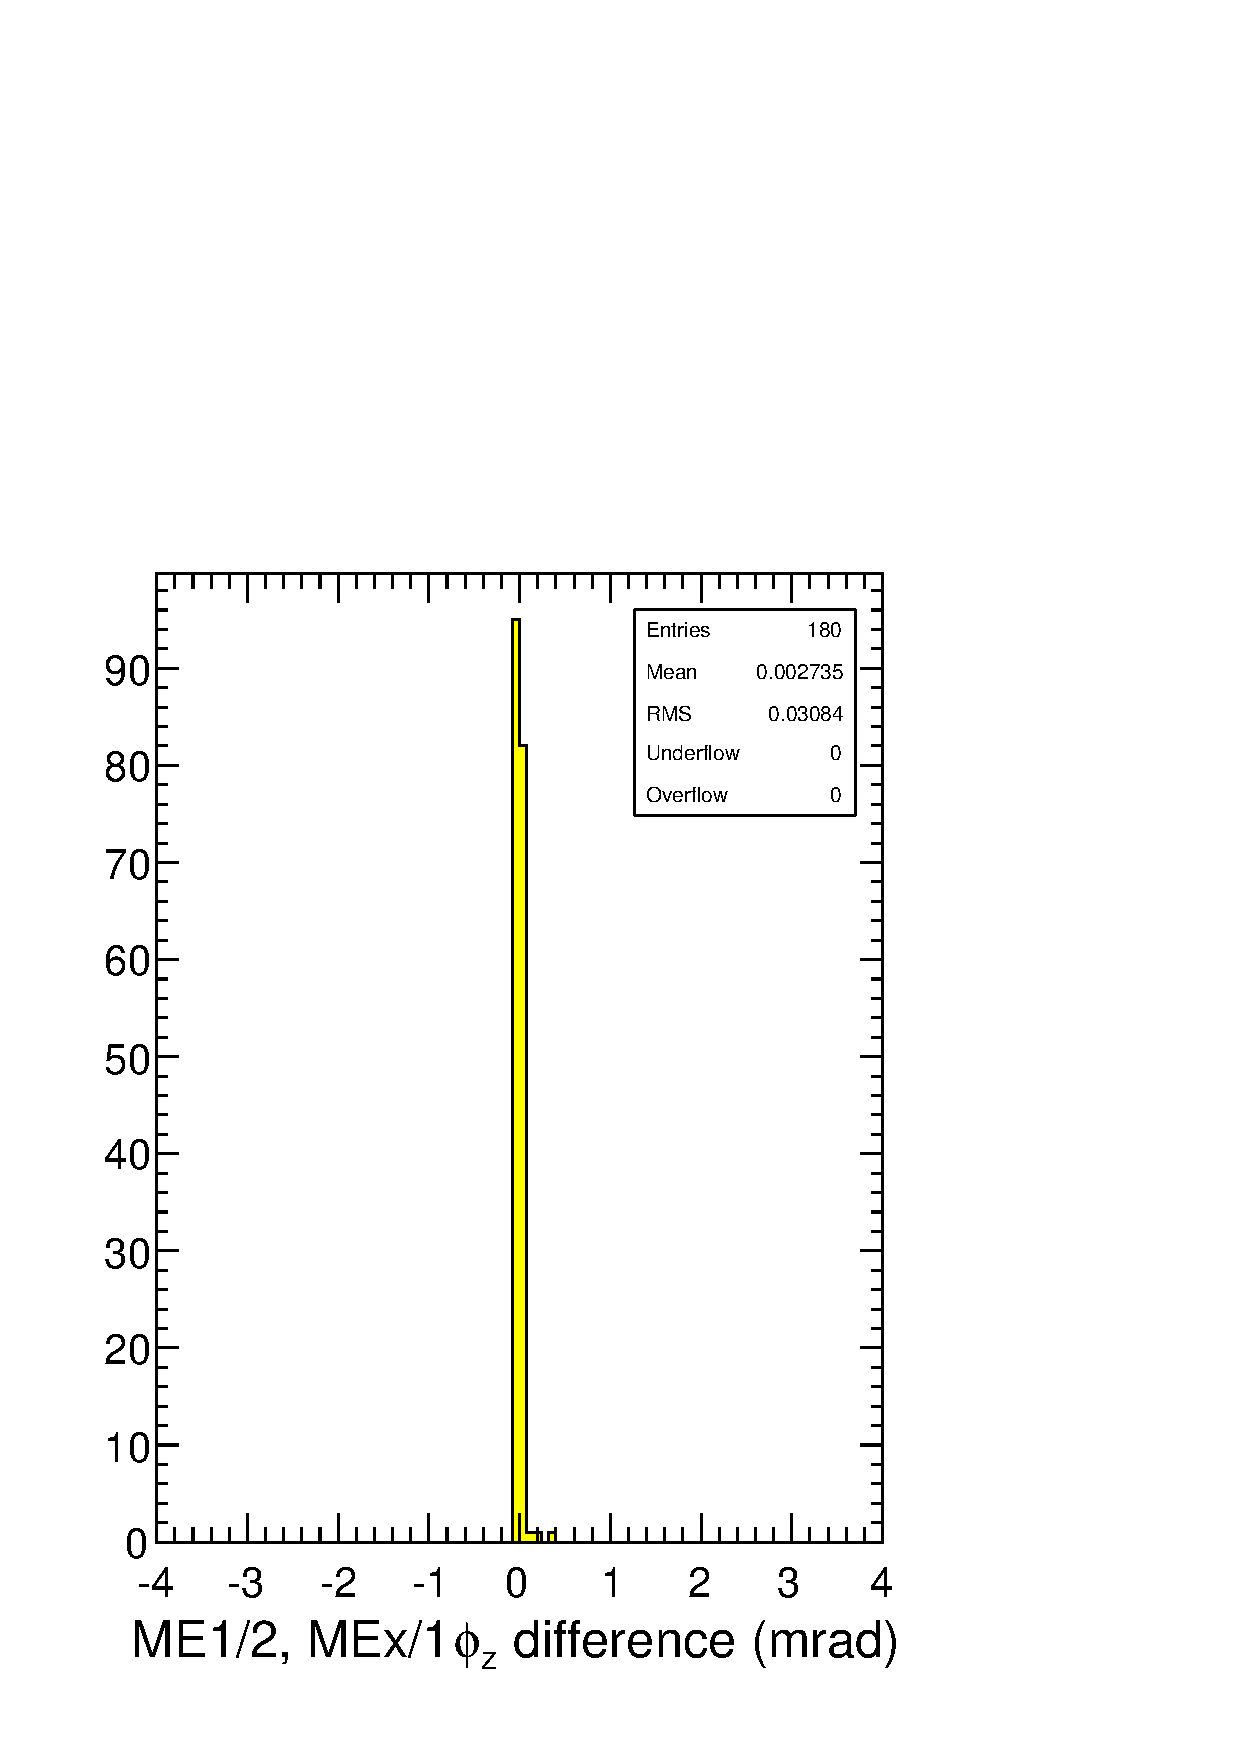
\includegraphics[width=0.32\linewidth]{noPhiYtoPhiY_phiz_inner.pdf}
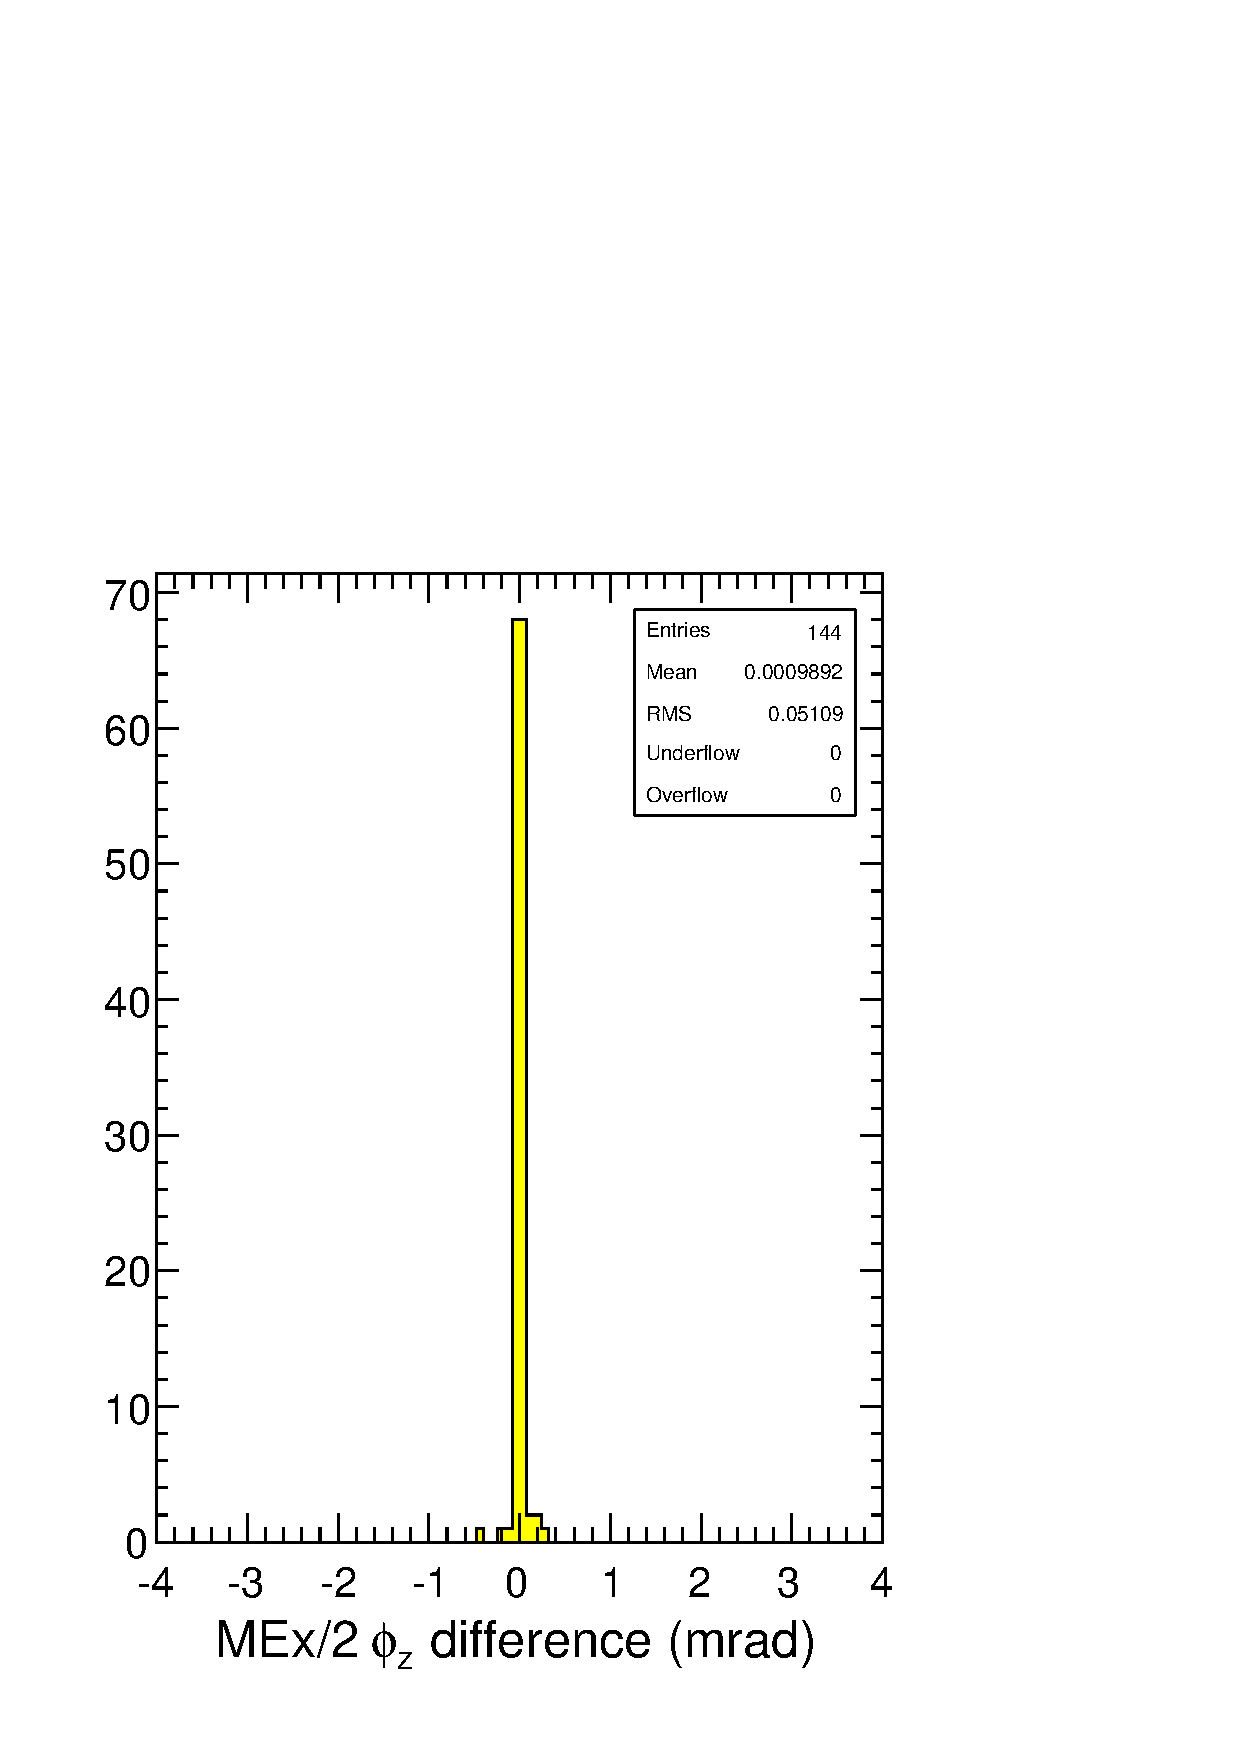
\includegraphics[width=0.32\linewidth]{noPhiYtoPhiY_phiz_outer.pdf}
\end{center}

\caption{Differences in $\phi_z$ parameters between a summer~2010
  alignment with and without $\phi_y$ pre-alignment.  All $\phi_z$
  differences are completely
  negligible. \label{fig:noPhiYtoPhiY_phiz_histograms}}
\end{figure}

\subsection{Comparison of results with and without PG constraint}

The effect of the PG constraint was tested by aligning the same data
(summer~2010) with and without the constraint.  Without the
constraint, groups of chambers connected by BH overlap data are
mutually aligned, but disconnected groups are allowed to float
relative to one another.  Figure~\ref{fig:withPGtoNoPG_histograms}
shows no difference in ME1/1 due to the fact that no PG constraint was
applied in either case, small differences in the inner chambers, which
are dominated by beam-halo measurements, and large differences in the
outer chambers.  By plotting each of the outer rings versus chamber
number (in the same figure), we see that these differences have clear
global patterns.  In ME$+$2/2, there are two independent groups, one
of which ranges between chambers 16 and 19 (inclusive) and floats
1--2~mm relative to the other group.  ME$+$3/2 has a global
deformation with an amplitude of 3~mm, and ME$-$3/2 has a global
deformation with an amplitude of 1~mm.  Similar plots for $\phi_z$ are
shown in Fig.~\ref{fig:withPGtoNoPG_phiz_histograms}.

The outer-ring differences between PG-constrained and
non-PG-constrained alignments look like weak modes, so we plot the
shapes of the eight weakest modes in each ring in
Fig.~\ref{fig:uncertainties_noPG_mep32} (non-PG-constrained
alignment).  Since ME$+$2/2 and ME$-$2/2 each have two disconnected
regions, they each have two trivial modes deriving from the Lagrange
multipliers: one represents the fact that rotations of the whole ring
are unconstrained and the other represents the fact that the two
disconnected regions are unconstrained relative to one another.
ME$+$3/2 and ME$-$3/2 each have one trivial mode due to unconstrained
rotations of the ring only.  In these plots, each of the normalized
modes has been multiplied by the uncertainty in the mode to give a
sense of how they compare to one another.  A table of the largest mode
in each ring and the sum in quadrature of all modes in each ring are
given in Table~\ref{tab:uncertainties}.  We see from this table that
outer ring statistical uncertainties are about ten times larger than
inner ring statistical uncertainties.

\begin{figure}
\begin{center}
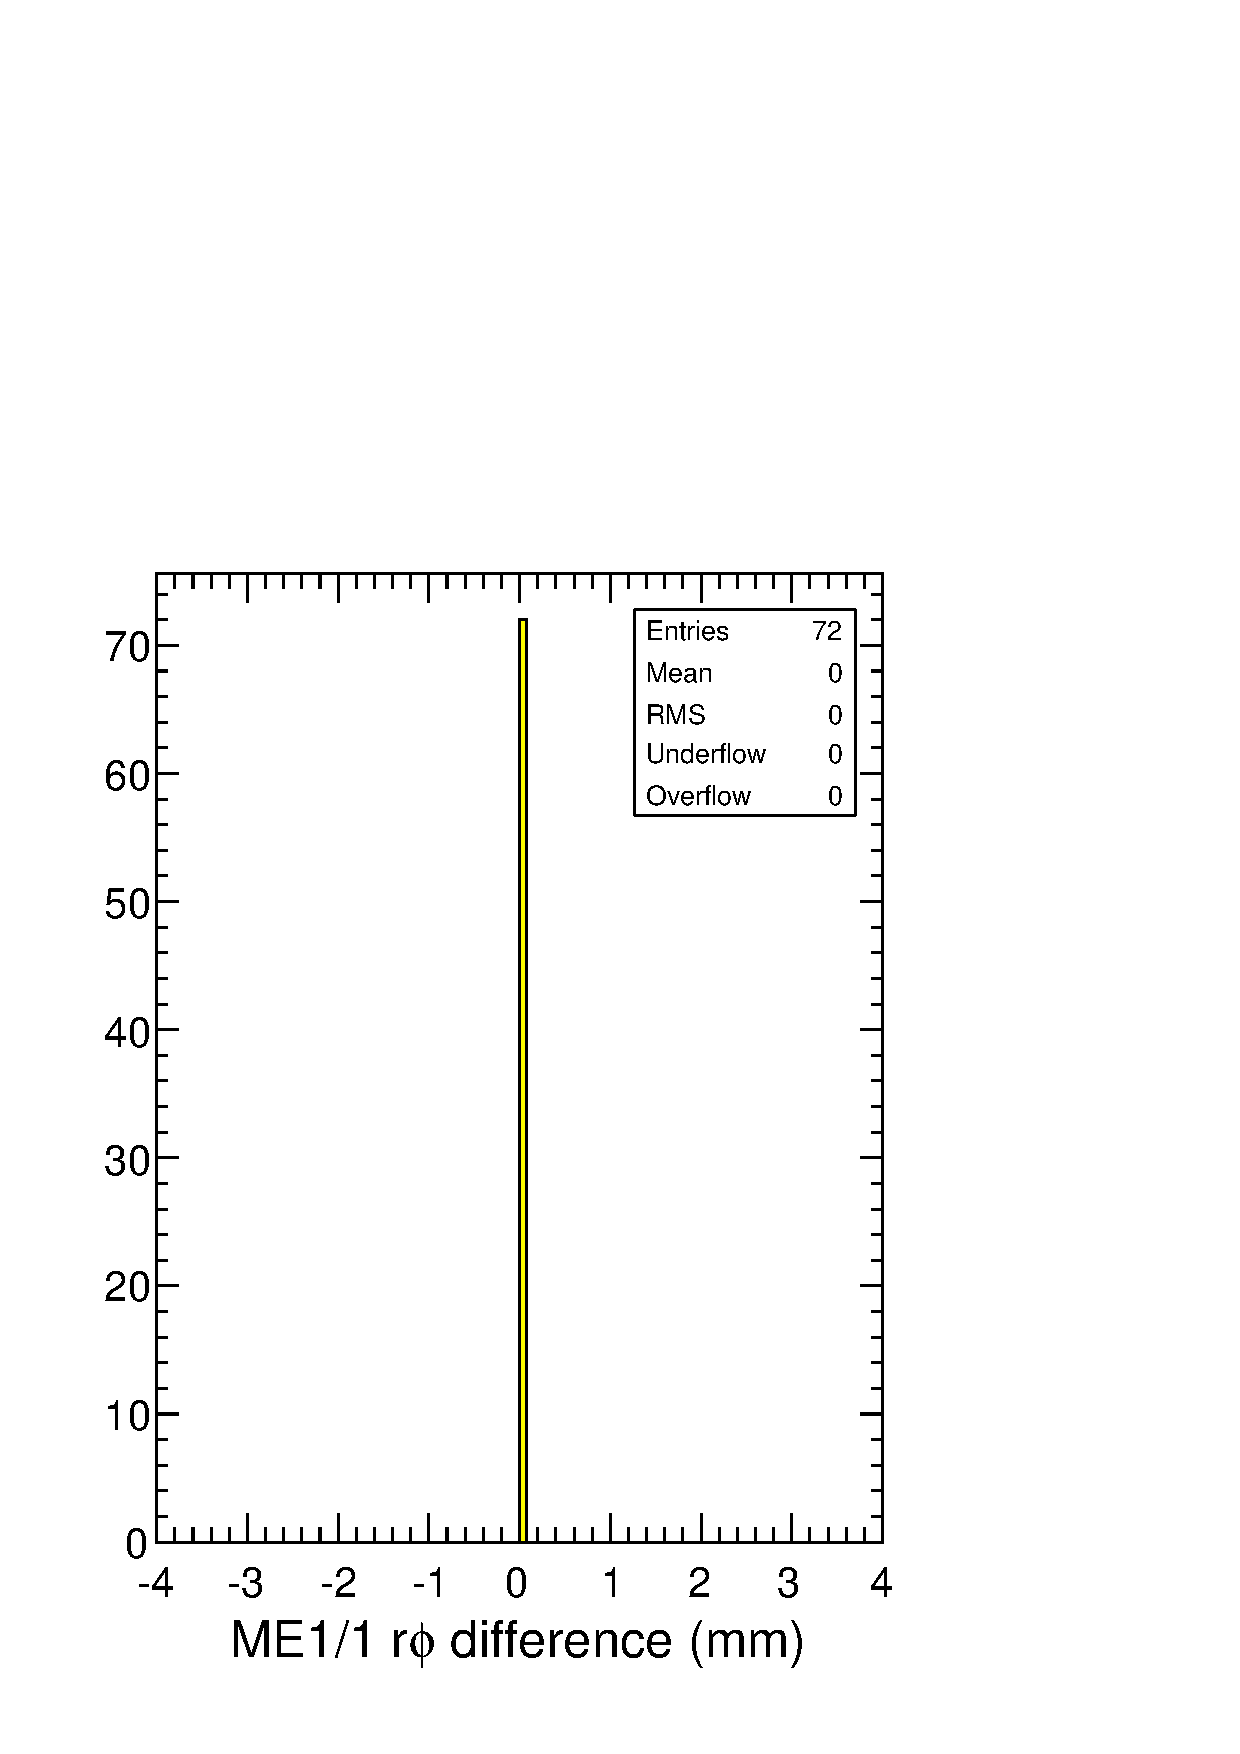
\includegraphics[width=0.32\linewidth]{withPGtoNoPG_me11.pdf}
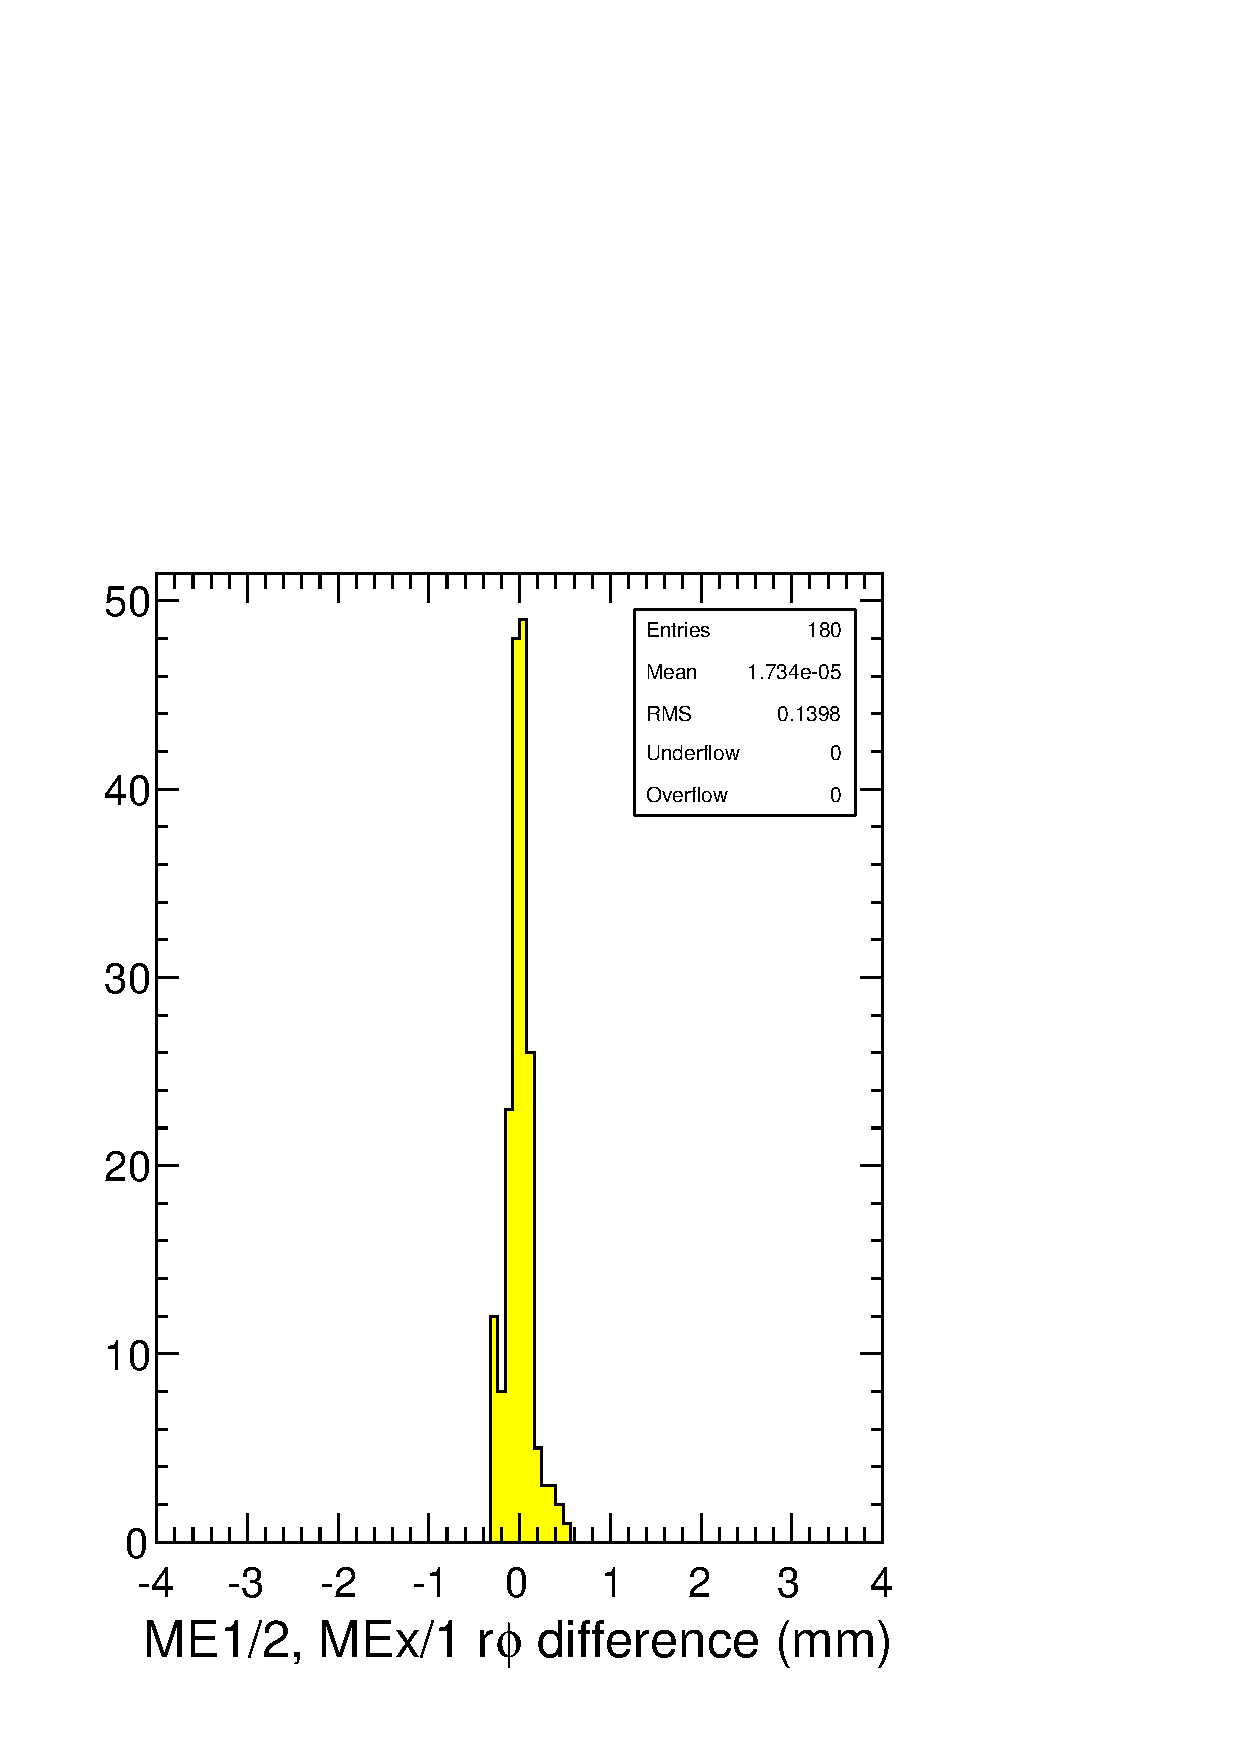
\includegraphics[width=0.32\linewidth]{withPGtoNoPG_inner.pdf}
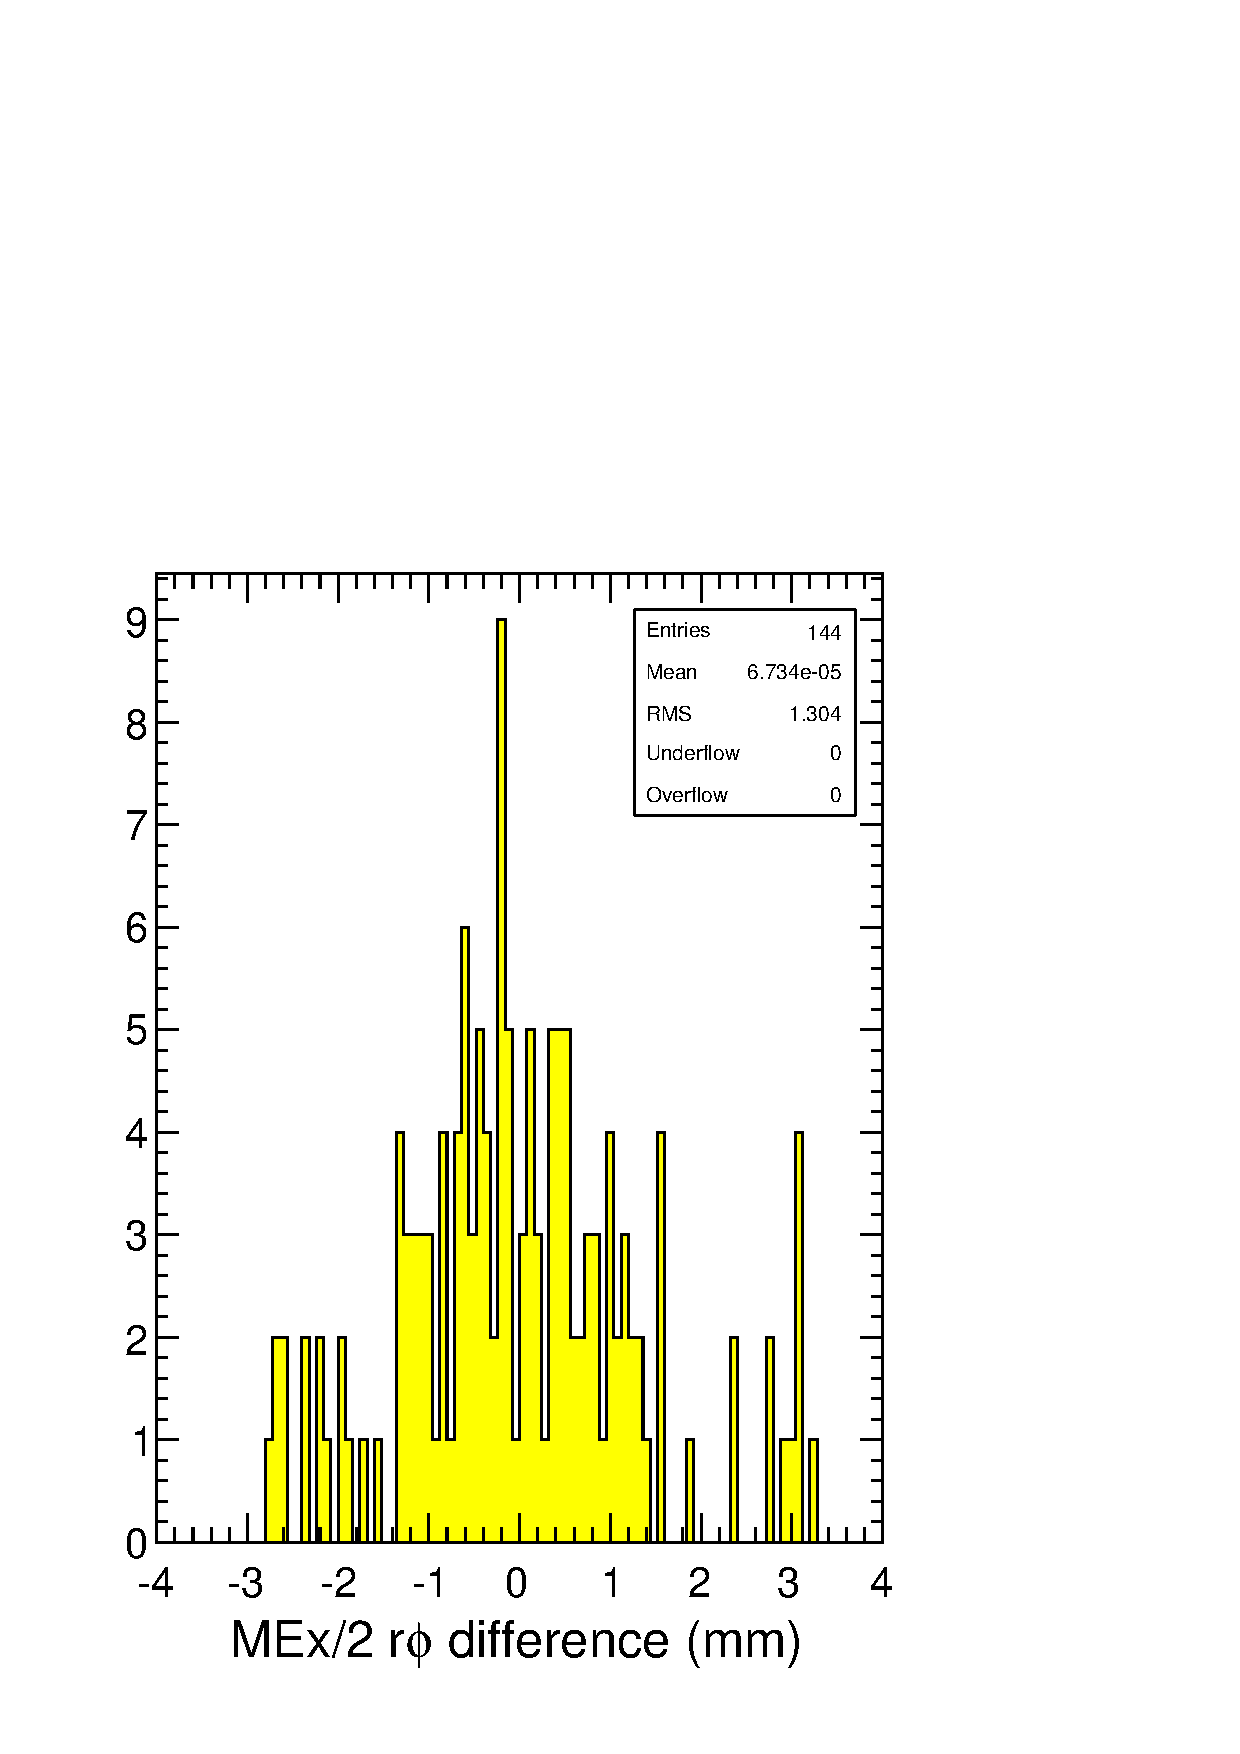
\includegraphics[width=0.32\linewidth]{withPGtoNoPG_outer.pdf}

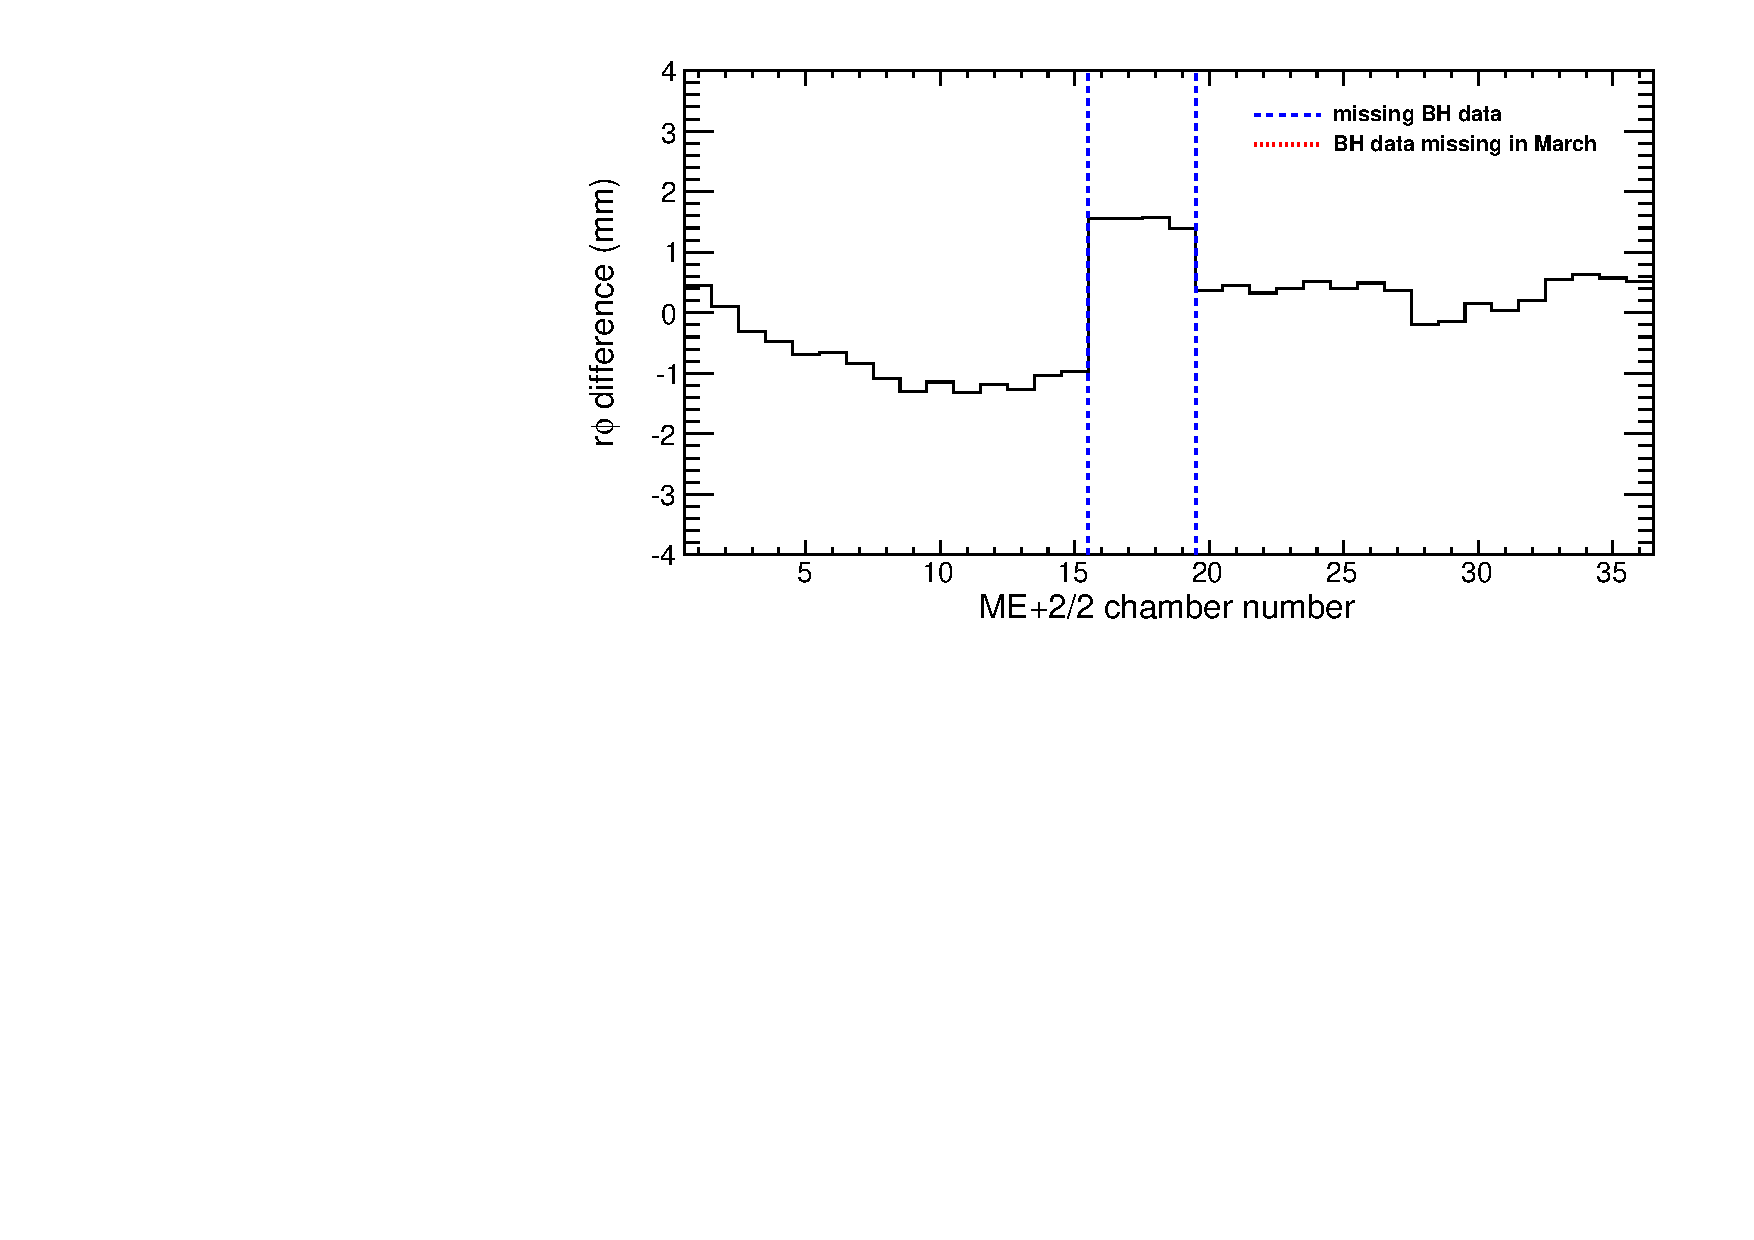
\includegraphics[width=0.45\linewidth]{withPGtoNoPG_mep22.pdf}
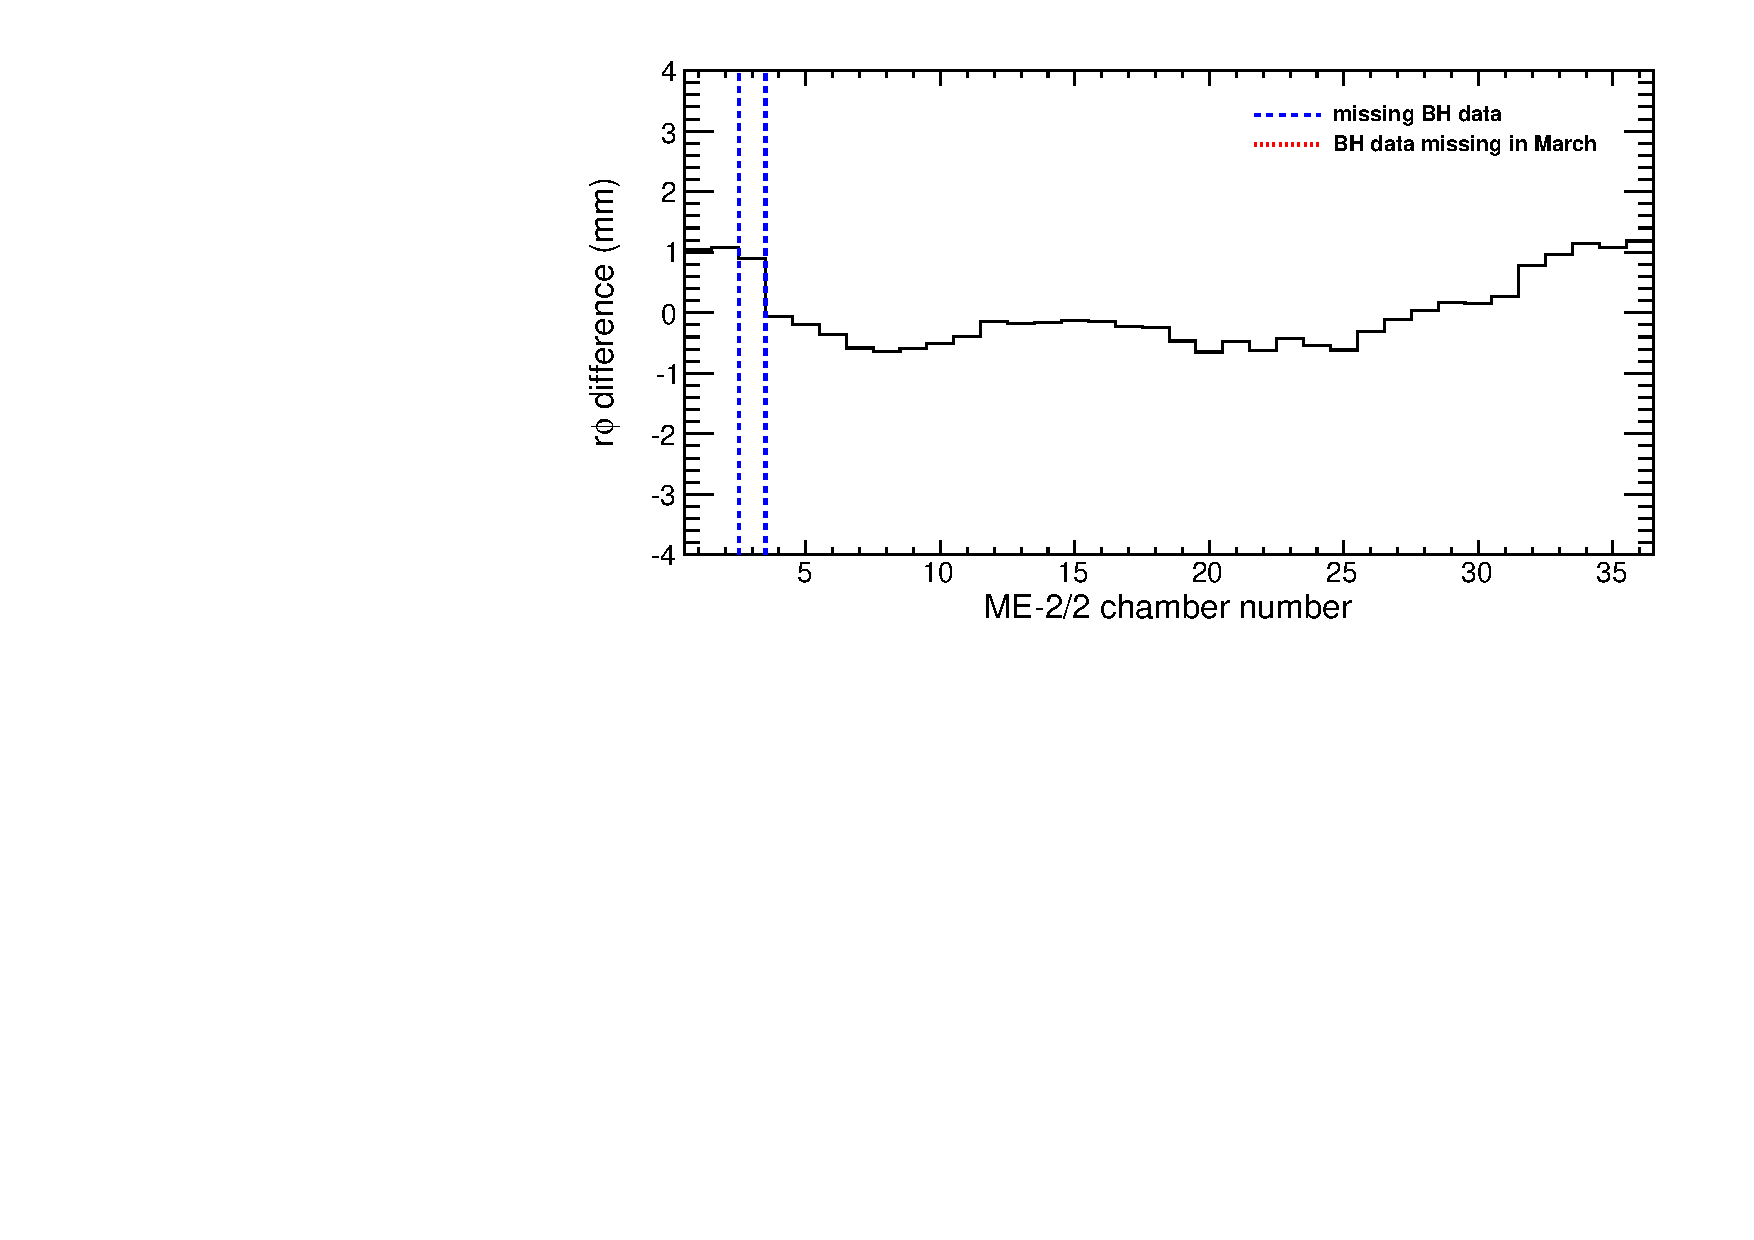
\includegraphics[width=0.45\linewidth]{withPGtoNoPG_mem22.pdf}

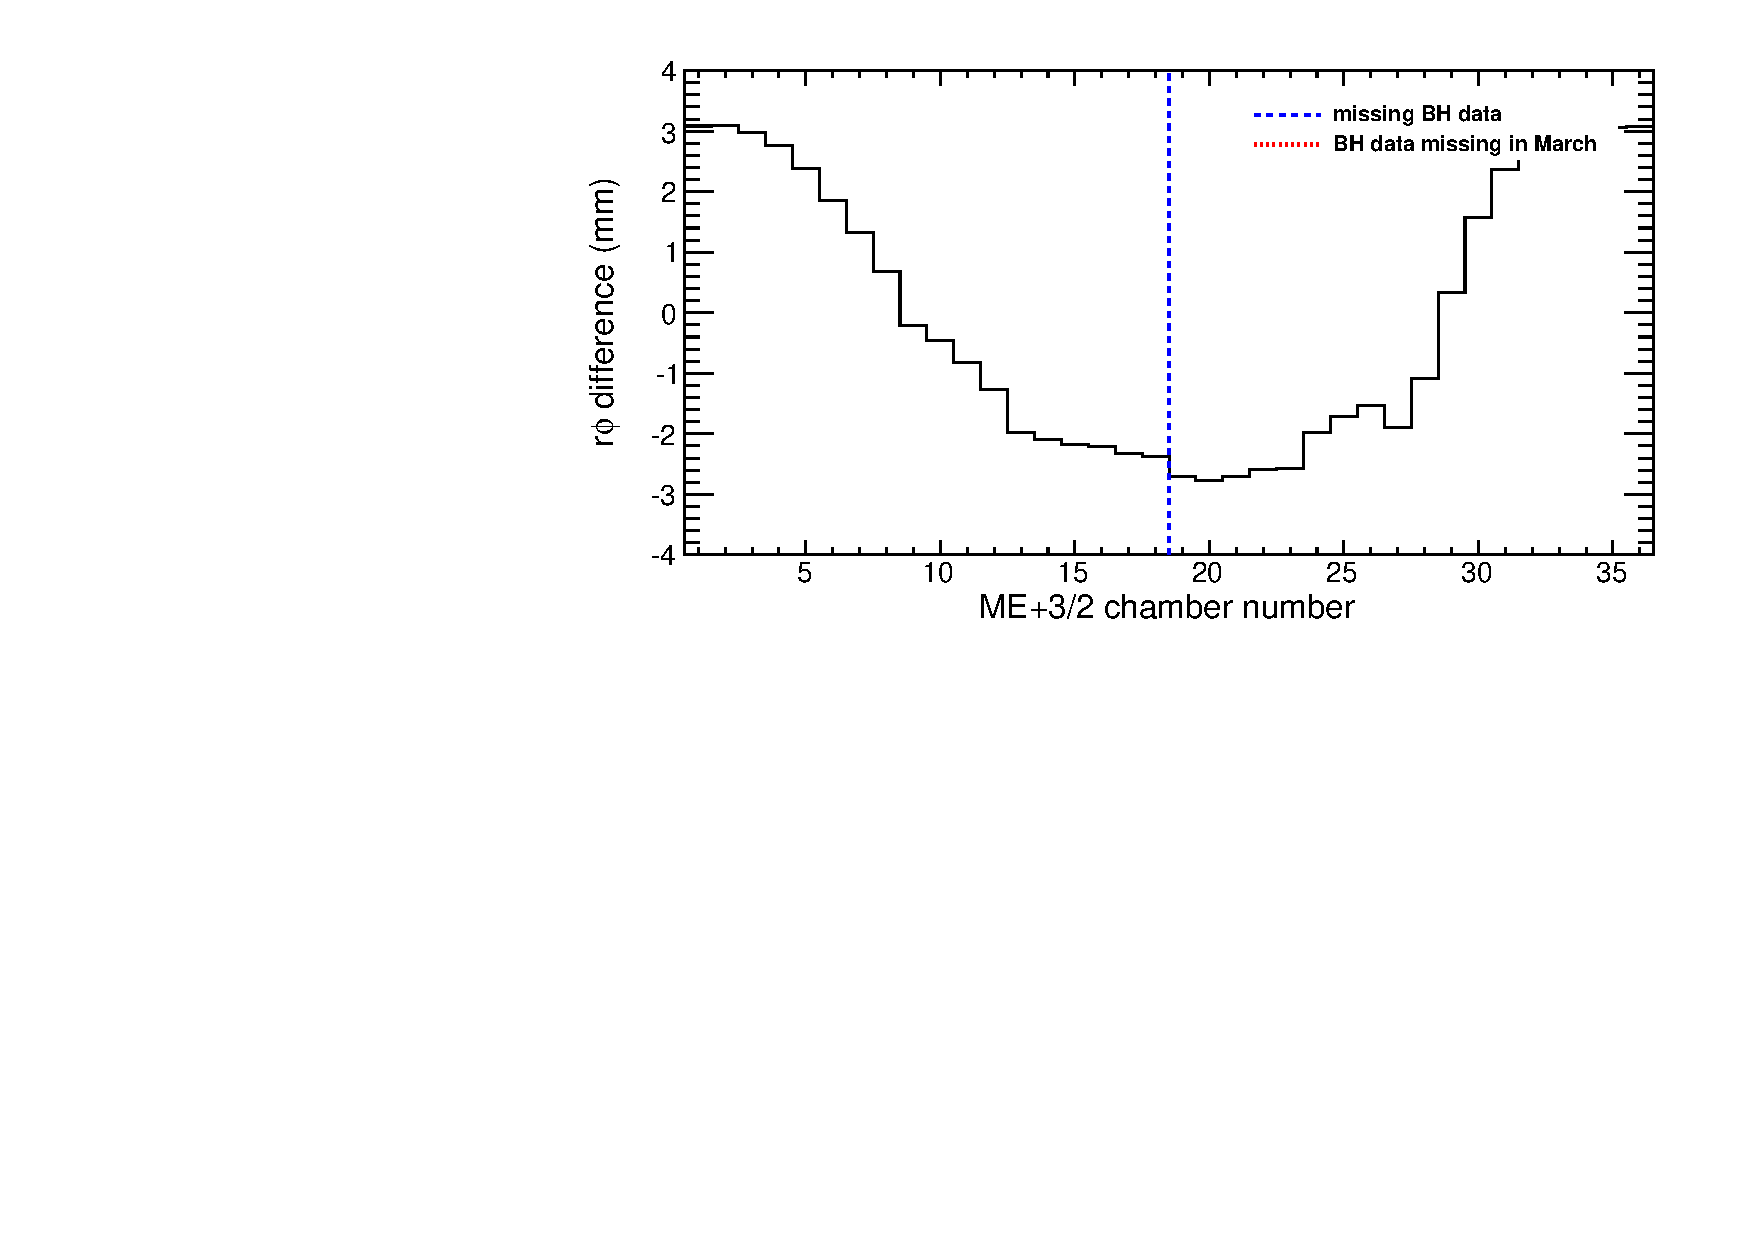
\includegraphics[width=0.45\linewidth]{withPGtoNoPG_mep32.pdf}
\includegraphics[width=0.45\linewidth]{withPGtoNoPG_mem32.pdf}
\end{center}

\caption{Differences in $r\phi$ parameters between a summer~2010
  alignment with and without PG constraint.  ME1/1 chambers have no
  PG constraint, so they are unaffected, and differences in
  inner-ring chambers are also negligible.  However, the outer rings
  differ systematically: ME$+$2/2 has two missing BH overlaps that
  benefit from the PG constraint, and ME$\pm$3/2 have global
  distortions that are suppressed by the PG constraint. \label{fig:withPGtoNoPG_histograms}}
\end{figure}

\begin{figure}
\begin{center}
\includegraphics[width=0.32\linewidth]{withPGtoNoPG_phiz_me11.pdf}
\includegraphics[width=0.32\linewidth]{withPGtoNoPG_phiz_inner.pdf}
\includegraphics[width=0.32\linewidth]{withPGtoNoPG_phiz_outer.pdf}
\end{center}

\caption{Differences in $\phi_z$ parameters between a summer~2010
  alignment with and without PG constraint.  ME1/1 chambers have no
  PG constraint, so they are unaffected.  Differences in other rings
  are at the level of 0.5--0.8~mrad (RMS). \label{fig:withPGtoNoPG_phiz_histograms}}
\end{figure}

\begin{figure}
\begin{center}
\includegraphics[width=0.45\linewidth]{uncertainties_noPG_mep22.pdf}
\includegraphics[width=0.45\linewidth]{uncertainties_noPG_mem22.pdf}

\includegraphics[width=0.45\linewidth]{uncertainties_noPG_mep32.pdf}
\includegraphics[width=0.45\linewidth]{uncertainties_noPG_mem32.pdf}
\end{center}

\caption{Statistical uncertainties in outer chambers without any PG
  constraint, expressed as uncorrelated normal modes.  Only the eight
  weakest (non-trivial) modes are shown.  Vertical dashed lines
  indicate neighboring chambers without BH data (and are therefore
  unconstrained).  \label{fig:uncertainties_noPG_mep32}}
\end{figure}

\begin{table}
\caption{Summary of uncertainties in alignment without PG constraint. \label{tab:uncertainties}}
\begin{center}
\begin{tabular}{c c c c}
Ring & Number of modes & Largest mode uncertainty & Sum in quadrature \\\hline
ME$+$1/1 & 32 modes & 1.13 mm & 1.69 mm \\
ME$+$1/2 & 32 modes & 0.44 mm & 0.62 mm \\
ME$+$2/1 & 17 modes & 0.15 mm & 0.19 mm \\
ME$+$2/2 & 34 modes & 1.40 mm & 1.74 mm \\
ME$+$3/1 & 17 modes & 0.08 mm & 0.14 mm \\
ME$+$3/2 & 35 modes & 1.62 mm & 2.00 mm \\
ME$+$4/1 & 17 modes & 0.16 mm & 0.21 mm \\
ME$+$4/2 & 3 modes  & 0.30 mm & 0.34 mm \\\hline
ME$-$1/1 & 32 modes & 0.86 mm & 1.28 mm \\
ME$-$1/2 & 34 modes & 0.55 mm & 0.73 mm \\
ME$-$2/1 & 17 modes & 0.16 mm & 0.20 mm \\
ME$-$2/2 & 34 modes & 1.44 mm & 1.73 mm \\
ME$-$3/1 & 17 modes & 0.09 mm & 0.14 mm \\
ME$-$3/2 & 35 modes & 0.83 mm & 1.15 mm \\
ME$-$4/1 & 17 modes & 0.09 mm & 0.15 mm
\end{tabular}
\end{center}
\end{table}

%% \begin{figure}
%% \begin{center}
%% \includegraphics[width=0.45\linewidth]{withPGtoNoPG_mep2_picture.pdf}
%% \end{center}
%% \caption{Differences in $x$, $y$, and $\phi_z$ between a summer~2010
%%   alignment with and without PG constraint for ME$+$2/2.  The two
%%   colors distinguish disconnected regions when aligning without a PG
%%   constraint: without a PG constraint, the red region is allowed to
%%   float independently of the blue region.  Compare to
%%   Fig.~\ref{fig:withPGtoNoPG_histograms}. \label{fig:withPGtoNoPG_mep2_picture}}
%% \end{figure}

There are two possible explanations for the global distortions in
ME$\pm$3/2:
\begin{itemize}
\item they are weak modes of the alignment procedure using BH data
  only, and are minimized by adding PG constraints;
\item they are a true deformation of the disk that occured sometime
  between 2007 (when the PG data were collected) and 2010 (when the BH
  data were collected).
\end{itemize}
The best way to resolve this question is to look at both geometries in
an independent dataset.  The 3~mm amplitude of ME$+$3/2 (and possibly
the 1~mm amplitude of ME$-$3/2) is large enough to be seen from
collisions.  This study is forthcoming.

\subsection{Comparison of results with and without PG used to fill
  missing BH overlaps only}

Since PG constraints are clearly needed to control floating groups of
chambers such as those in ME$+$2/2, but might be unrealistically
distorting the shapes of rings such as ME$+$3/2, it would be good to
compromise by applying PG constraints only where they are needed:
directly around the missing BH data.  Referring to
Fig.~\ref{fig:occupancy_March2010} to identify missing overlaps, we
find that only 25 chambers strictly need to be constrained, out of 299
available constraints.  These are listed in Table~\ref{tab:pgholes}.

\begin{table}
\caption{PG data used to fill holes in BH overlaps data. \label{tab:pgholes}}
\begin{center}
\begin{tabular}{l}
ME$+$4/1/14 and ME$+$4/1/15 \\
ME$+$3/2/18 and ME$+$3/2/19 \\
ME$+$2/2/15 and ME$+$2/2/17 (16 has no BH or PG data) \\
ME$+$2/2/19 and ME$+$2/2/20 \\
ME$+$2/1/01 and ME$+$2/1/02 \\
ME$+$1/2/14, ME$+$1/2/15, and ME$+$1/2/16 \\
ME$+$1/2/34, ME$+$1/2/36, and ME$+$1/2/01 (35 has no BH or PG data) \\
ME$-$1/2/04 and ME$-$1/2/05 \\
ME$-$1/2/33 and ME$-$1/2/34 \\
ME$-$2/1/06 and ME$-$2/1/07 \\
ME$-$2/2/02, ME$-$2/2/03, and ME$-$2/2/04
\end{tabular}
\end{center}
\end{table}

The results of an alignment using only these few constraints, compared
to an alignment with all chambers constrained, are shown in
Figs.~\ref{fig:withPGtoPGholes_histograms} and
\ref{fig:withPGtoPGholes_phiz_histograms}.  They look very similar to
the comparison of non-PG-constrained with fully PG-constrained in
Figs.~\ref{fig:withPGtoNoPG_histograms} and
\ref{fig:withPGtoNoPG_phiz_histograms}, except that chambers 16--19
(inclusive) in ME$+$2/2 are not allowed to float freely with respect
to the other chambers in this ring, and the discontinuity between
chambers 18 and 19 in ME$+$3/2 is smaller--- both of which are gaps in
BH data.

\begin{figure}
\begin{center}
\includegraphics[width=0.32\linewidth]{withPGtoPGholes_me11.pdf}
\includegraphics[width=0.32\linewidth]{withPGtoPGholes_inner.pdf}
\includegraphics[width=0.32\linewidth]{withPGtoPGholes_outer.pdf}

\includegraphics[width=0.45\linewidth]{withPGtoPGholes_mep22.pdf}
\includegraphics[width=0.45\linewidth]{withPGtoPGholes_mem22.pdf}

\includegraphics[width=0.45\linewidth]{withPGtoPGholes_mep32.pdf}
\includegraphics[width=0.45\linewidth]{withPGtoPGholes_mem32.pdf}
\end{center}

\caption{Differences in $r\phi$ parameters between a summer~2010
  alignment with and without PG measurements used to fill missing BH
  overlaps only.  ME1/1 chambers have no PG constraint, so they are
  unaffected, and differences in inner-ring chambers are also
  negligible.  However, the outer rings differ systematically.
  ME$+$2/2 has two missing BH overlaps that benefit from the PG
  constraint: with only these constraints applied, discontinuities at
  chambers 15-16 and 19-20 are less significant (compare with
  Fig.~\ref{fig:withPGtoNoPG_histograms}).  Global distortions in
  ME$\pm$3/2 are unaffected. \label{fig:withPGtoPGholes_histograms}}
\end{figure}

\begin{figure}
\begin{center}
\includegraphics[width=0.32\linewidth]{withPGtoPGholes_phiz_me11.pdf}
\includegraphics[width=0.32\linewidth]{withPGtoPGholes_phiz_inner.pdf}
\includegraphics[width=0.32\linewidth]{withPGtoPGholes_phiz_outer.pdf}
\end{center}

\caption{Differences in $\phi_z$ parameters between a summer~2010
  alignment with and without PG measurements used to fill the missing
  BH overlaps only.  ME1/1 chambers have no PG constraint, so they are
  unaffected.  Differences in other rings are at the level of
  0.5--0.8~mrad (RMS). \label{fig:withPGtoPGholes_phiz_histograms}}
\end{figure}

The global distortions between minimally PG-constrained and fully
PG-constrained alignments in ME$\pm$3/2 are presented graphically in
Fig.~\ref{fig:withPGtoPGholes_me3_picture}.  These are exaggerated
pictoral representations (by a factor of 200) of the geometry
differences, showing differences in $x$, $y$, and $\phi_z$.  The
chambers are colored by $x$ differences as a guide to the eye: the new
information in this plot is the correlation between $r\phi$ and
$\phi_z$ deviations, which are maximal at the bottom of the rings.

\begin{figure}
\begin{center}
\includegraphics[width=0.45\linewidth]{withPGtoPGholes_mep3_picture.pdf}
\includegraphics[width=0.45\linewidth]{withPGtoPGholes_mem3_picture.pdf}
\end{center}
\caption{Differences in $x$, $y$, and $\phi_z$ between a summer~2010
  alignment with and without PG measurements used to fill the missing
  BH overlaps only, for ME$\pm$3/2.  The color gradation signifies the
  difference in $x$, and is meant to help the eye see the pattern of
  correlated $x$ and $\phi_z$ deviations near the bottom of ME$+$3/2.
  Compare to
  Fig.~\ref{fig:withPGtoPGholes_histograms}.  \label{fig:withPGtoPGholes_me3_picture}}
\end{figure}

\subsection{Ring radii measured from closure constraints}

The first step in each beam-halo alignment is to adjust the radius of
each ring such that the sum of $r\phi$ residuals means is zero
($\sum_i m_{i\,i+1} = 0$ for BH $r\phi$ constraints).  Without this
correction, the alignment results would buckle to try to distribute
the non-zero sum across non-uniform weights.  Since we interpret this
correction as a physical change in the radius of rings (expected in
$\vec{B}=3.8$~T), these ring-radius corrections are also interesting
results.

Table~\ref{tab:radiuscorrections} summarizes ring-radius corrections
for all alignments considered in this note.  It is worth noting that
the new hardware description (believed to be more accurate than the
old one for reasons not discussed here) significantly changes
the apparent radius of some rings, in all cases making changes
relative to design less extreme.  Corrections to $\phi_x$ can change
the radial position of $r\phi$ intercepts at the plane between pairs
of chambers, modifying the apparent radius.

\begin{table}
\caption{Radius corrections relative to the following nominal values:
  ME1/1 1815~mm, ME1/2 3697~mm, ME2/1 2427~mm, ME2/2 5265~mm, ME3/1
  2527~mm, ME3/2 5265~mm, ME4/1 2626.5~mm, where positive corrections
  mean that the radius must be made larger.  The four geometries below
  are ``PG only,'' no beam-halo radius correction, ``with old HW,''
  beam-halo alignment starting from the old hardware $z$/$\phi_x$
  pre-alignment, ``with new HW,'' beam-halo alignment starting from
  the new hardware $z$/$\phi_x$, ``new HW and $\phi_y$,'' beam-halo
  alignment starting from the new hardware and non-zero $\phi_y$
  corrections from collisions. \label{tab:radiuscorrections}}
\begin{center}
\begin{tabular}{c r r r r}
& PG only & with old HW & with new HW & new HW and $\phi_y$ \\\hline
ME$+$1/1 &  $0.0$ & $-0.5$ & $-0.5$ & $-0.5$ \\
ME$+$1/2 &  $0.3$ &  $1.8$ &  $0.8$ &  $0.7$ \\
ME$+$2/1 &  $0.8$ &  $2.0$ &  $2.1$ &  $2.0$ \\
ME$+$2/2 &  $1.0$ & $-0.4$ &  $1.8$ &  $2.0$ \\
ME$+$3/1 & $-0.8$ & $-1.3$ & $-1.1$ & $-1.1$ \\
ME$+$3/2 & $-0.3$ & $-5.4$ & $-2.0$ & $-2.0$ \\
ME$+$4/1 & $-0.4$ & $-1.2$ & $-1.2$ & $-1.2$ \\\hline
ME$-$1/1 &  $0.0$ & $-1.7$ & $-1.7$ & $-1.7$ \\
ME$-$1/2 & $-0.3$ &  $0.4$ &  $0.4$ &  $0.3$ \\
ME$-$2/1 &  $0.0$ &  $1.0$ &  $0.9$ &  $1.0$ \\
ME$-$2/2 &  $0.7$ & $-0.7$ &  $0.5$ &  $0.4$ \\
ME$-$3/1 & $-1.2$ & $-2.0$ & $-2.0$ & $-2.0$ \\
ME$-$3/2 & $-0.7$ & $-5.1$ & $-3.8$ & $-3.9$ \\
ME$-$4/1 & $-0.6$ & $-1.5$ & $-1.4$ & $-1.5$ \\
\end{tabular}
\end{center}
\end{table}

\section{Conclusions and recommended geometry}

The beam-halo overlaps alignment method is now a standard technique,
having been applied four times since first LHC beams in 2008.  Most
recently, beam-halo data collected during summer~2010 collisions were
analyzed.  Seven ME1/1 chambers that were inoperative during the
March~2010 dedicated beam-halo run are now available, and one chamber
in ME$-$1/2 is now missing.  Photogrammetry data are used to constrain
rings with missing beam-halo data.

In this note, we studied differences in the apparent geometry between
March and summer~2010, but due to changes in trigger conditions,
collisions backgrounds, and available chambers, these differences
cannot be conclusively identified as being real motions of the
detectors.  In the case of ME$+$1/1, they can clearly be identified as
improvements due to the addition of previously unavailable beam-halo data.

Since two new pre-alignments (hardware $z$/$\phi_x$ and collisions
$\phi_y$) are to be applied to the new alignment, we studied the
effect of applying each correction before beam-halo alignment.
Differences were all significantly less than 1~mm in $r\phi$ and
1~mrad in $\phi_z$.  The new hardware correction has a significant
influence on apparent ring-radii, though.

The photogrammetry constraint was studied in more detail than in
previous alignment work, with three cases considered: (1)~apply all PG
data, (2)~only apply PG data to fill in gaps in the BH data, and
(3)~apply no PG data.  The alignment clearly suffers in case (3), most
visibly in ME$+$2/2 (Fig.~\ref{fig:withPGtoNoPG_histograms}).  Cases
(1) and (2) only differ in the outer rings, as PG are not available in
ME1/1 and inner rings are statistically dominated by BH data.
Applying or not applying full PG data changes the global shapes of
outer rings, especially ME$+$3/2.  To determine whether the global
distortion is a weak mode of the minimally PG-constrained alignment
or a real coherent motion between 2007 and 2010, we should observe
both in collisions data and look for the presence or absence of a 3~mm
amplitude trend.

SQLite files representing the two cases can be found at:
\begin{itemize}
\item {\tt /afs/cern.ch/user/p/pivarski/public/OCT23\_PG-HW-phiy-BHPG.db} (1);
\item {\tt /afs/cern.ch/user/p/pivarski/public/OCT23\_PG-HW-phiy-BHPGholes.db} (2).
\end{itemize}
One of these two will be proposed for the sign-off on Nov.~5,
depending on the outcome of the test with collisions muons.  It will
also be necessary to apply disk corrections to finalize the alignment.

\end{document}
